
% WARNING!  Do not type any of the following 10 characters except as directed:
%                &   $   #   %   _   {   }   ^   ~   \
%
%%
%%  default option for pdfx.sty  if not specified on the command-line.
\providecommand{\pdfxopt}{a-1b}
%%
%%  Use  {filecontents}  for the  .xmpdata file before input encoding is specified.
%%
%%%%%%%%%%%%%%%%%%%%%%%%%%%%%%%%%%%%%%%%%%%%%%%%%%%
\begin{filecontents*}{\jobname.xmpdata}
	% a macro definition, used below
	\pdfxEnableCommands{% simple macro definitions can be provided everything expands to characters
	 \def\RossPete{Ross \& Pete}
	 }
	\Title{Linear Algebra (\jobname)}%  *not* set by LaTeX's  \title
	\Author{Jason Siefken\sep et al.}% *not* set by LaTeX's \author
	\Subject{Linear Algebra textbook/workbook}
	\Keywords{linear algebra\sep vectors\sep mathematics\sep textbook}
	\Org{University of Toronto}
	\CreatorTool{LaTeX + pdfx.sty with options \pdfxopt}
	\Copyright{Jason Siefken}
	\WebStatement{https://github.com/siefkenj/IBLLinearAlgebra/}% should be URL to copyright statement on the web
	\CoverDisplayDate{2019}
	\CoverDate{2019-08-014}%  must be in format  YYYY-MM-DD  or  YYYY-MM
	\Doi{0.0.0.0}%
	%
	% setting the color profile, these reproduce the defaults; use your own, if required
	%
	% RGB is used with PDF/A (4 parameters):
	\setRGBcolorprofile{sRGB_IEC61966-2-1_black_scaled.icc}{sRGB_IEC61966-2-1_black_scaled}{sRGB IEC61966 v2.1 with black scaling}{http://www.color.org}
	%
	%  For Adobe Color Profiles, set the directory for your system
	%
	%  e.g.  on Mac OS X
	%  What is it under Windows ?
	%
	\gdef\ColorProfileDir{./common/}
	% 
	%  For available profiles, see file  AdobeColorProfiles.tex
	%  For PDF/X-4p or PDF/X-5pg   see file  AdobeExternalProfiles.tex
	%
	%  Now you can use the macros defined in those files:
	 \FOGRAXXXIX
	%
	% or CMYK is used with  PDF/X (4 parameters)
	% \setCMYKcolorprofile{\ColorProfileDir coated_FOGRA39L_argl.icc}{Coated FOGRA39}{FOGRA39 (ISO Coated v2 300\%\space (ECI))}{http://www.color.org}
\end{filecontents*}

\documentclass{workbook}


% pdfx will set color profile etc. information appropriately, so the pdf renders
% consistently across devices. But, it doesn't work with the xelatex-based tectonics
\usepackage{ifxetex}
	\usepackage[utf8]{inputenc}
\ifxetex
\else
	\usepackage[a-3u]{pdfx}
\fi

%%%
% import all needed packages and macros
%%%
\usepackage[yyyymmdd]{datetime}
%%
%% All packages and macros needed for the problemsets
%%

\usepackage{amsmath}

\usepackage{lipsum}
%\usepackage{showframe}
%\usepackage{layout}


\usepackage[charter,cal=cmcal]{mathdesign} %different font
%\usepackage{avant}

\usepackage{microtype}
\usepackage{mathtools}
\usepackage{etoolbox}
%\usepackage{amsfonts}
%\usepackage{amssymb}
\usepackage{graphicx}
\graphicspath{{images/}}
\usepackage[inline]{enumitem}
\usepackage{xparse}
\usepackage{ifthen}
\usepackage{caption}
\usepackage{subcaption}
\usepackage{tikz}
	\usetikzlibrary{fit}
	\usetikzlibrary{fadings}
	\usetikzlibrary{calc}
	\tikzset{>=latex}
	\usetikzlibrary{cd}
	\usetikzlibrary{spy}
	\usetikzlibrary{patterns}
	\usetikzlibrary{decorations, decorations.pathreplacing, decorations.markings}

\usepackage{fancyhdr}
\usepackage{calc}
\usepackage{wrapfig}
\usepackage{marginnote}
\usepackage{mparhack}
\usepackage{marginfix}
\usepackage{indextools}
\usepackage[open=false]{bookmark}  % render the pdf TOC in the proper order
\hypersetup{
	hidelinks=true,
	linkcolor = {0 0 1},
	unicode=true,
	psdextra=true,
}
\usepackage{common/nicematrix}

%\usepackage[
%  linktocpage=false,      % no page numbers are clickable
%  colorlinks=false,       % no color
%  breaklinks=true,        % break URLs
%  bookmarks,              % creates bookmarks in pdf
%  hyperfootnotes=true,    % clickable footnotes
%  pdfborder={0 0 0},      % for removing borders around links
%  bookmarksnumbered=true, % If Acrobat bookmarks are requested, include section numbers.
%  bookmarksopen=false,    % If Acrobat bookmarks are requested, show them with all the subtrees expanded.
%  %hidelinks=true,
%  %linkcolor=blue,
%  %citecolor=blue,
%  %urlcolor=blue,
%  pdfpagemode={UseOutlines}, % show pdf bookmarks (indices) on startup; does not function all the time
%  pdftitle={...}, % title
%  pdfauthor={...}, % author
%  pdfkeywords={...}, % subject of the document
%  pdfsubject={...}, % list of keywords
%  pdfmenubar=true,        % make PDF viewer’s menu bar visible
%  pdfpagelabels,
%]{hyperref}
%\usepackage[hidelinks,]{hyperref}
\usepackage{fnpct} % fancy footnote spacing
\usepackage{bm}
\usepackage{systeme}
\usepackage{datatool}% http://ctan.org/pkg/datatool for sorted lists
\usepackage{xspace}


\usepackage{pgfplots}
\pgfplotsset{compat=1.16}
	\usepgfplotslibrary{fillbetween}
%%%
% Useful Linear Algebra macros
%%%
\newcommand{\declarecommand}[1]{\providecommand{#1}{}\renewcommand{#1}}
\DeclareDocumentCommand{\R}{}{\mathbb{R}}  % we don't care if it's already defined.  We really want *this* command!
\DeclareDocumentCommand{\Z}{}{\mathbb{Z}}
\DeclareDocumentCommand{\Q}{}{\mathbb{Q}}
\DeclareDocumentCommand{\N}{}{\mathbb{N}}
\DeclareDocumentCommand{\C}{}{\mathbb{C}}
\DeclareDocumentCommand{\d}{}{\mathrm{d}}
\DeclareDocumentCommand{\dd}{}{\mathbbm{d}} % exterior derivative
\DeclareMathOperator{\Span}{span}
\DeclareMathOperator{\Img}{img}
\DeclareMathOperator{\Id}{id}
\DeclareMathOperator{\Ident}{\Id}
\DeclareMathOperator{\Vol}{Vol}
\DeclareMathOperator{\VolChange}{Vol\hspace{1.5pt}Change}
\DeclareMathOperator{\Range}{range}
\DeclareMathOperator{\Rref}{rref}
\DeclareMathOperator{\Rank}{rank}
\DeclareMathOperator{\Comp}{\Vcomp}
\DeclareMathOperator{\Vcomp}{v\hspace{1pt}comp}
\DeclareMathOperator{\Null}{null}
\DeclareMathOperator{\Nullity}{nullity}
\DeclareMathOperator{\Char}{char}
\DeclareMathOperator{\Proj}{proj}
\DeclareMathOperator{\Flux}{Flux}
\DeclareMathOperator{\Circ}{Circ}
\DeclareMathOperator{\chr}{char}
\DeclareMathOperator{\Dim}{dim}
\DeclareMathOperator{\Perp}{perp}
\DeclareMathOperator{\Ker}{kernel}
\DeclareMathOperator{\Row}{row}
\DeclareMathOperator{\Col}{col}
\DeclareMathOperator{\Rep}{Rep}
\newcommand{\BasisChange}[2]{[#2\!\leftarrow\!#1]}
\newcommand{\proj}{\Proj}
\newcommand{\rref}{\Rref}
\newcommand{\xhat}{{\vec e_1}}
\newcommand{\yhat}{{\vec e_2}}
\newcommand{\zhat}{{\vec e_3}}
\newcommand{\sbasis}[1]{\vec { e}_{#1}}
\newcommand{\mat}[1]{\begin{bmatrix*}[r]#1\end{bmatrix*}}
\newcommand{\matc}[1]{\begin{bmatrix}#1\end{bmatrix}}
\newcommand{\formarg}[2]{\big(#1;\, #2\big)}
\DeclarePairedDelimiter\abs{\lvert}{\rvert}
\DeclarePairedDelimiter\Abs{\lvert}{\rvert}
\DeclarePairedDelimiter\norm{\lVert}{\rVert}
\newcommand{\Norm}[1]{\norm{#1}}
% just to make sure it exists
\providecommand\given{}
% can be useful to refer to this outside \Set
\newcommand\SetSymbol[1][]{%
	\nonscript\::%
	\allowbreak
	\nonscript\:
	\mathopen{}}
\DeclarePairedDelimiterX\Set[1]\{\}{%
	\renewcommand\given{\SetSymbol[\delimsize]}
	#1
}
\newcommand{\Rrefto}{\xrightarrow{\text{row reduces to}}}


% redefine bmatrix,etc to allow optional argument for augmenting
% code from https://tex.stackexchange.com/questions/2233/whats-the-best-way-make-an-augmented-coefficient-matrix
\makeatletter
\renewcommand*\env@matrix[1][*\c@MaxMatrixCols c]{%
  \hskip -\arraycolsep
  \let\@ifnextchar\new@ifnextchar
  \array{#1}}
\makeatother

\newcommand{\scaledgrid}[1]{%
	\begin{tikzpicture}[scale=#1]
		\draw[thin, white!20!black, dotted] (-4.1,-4.1) grid (4.1,4.1);
		\draw[ <->] (-4.3,0) -- (4.3,0);
		\draw[ <->] (0,-4.3) -- (0,4.3);
	\end{tikzpicture}
}
\newcommand{\scaledshortgrid}[1]{%
	\begin{tikzpicture}[scale=#1]
		\draw[thin, white!20!black, dotted] (-4.1,-2.1) grid (4.1,2.1);
		\draw[ <->] (-4.3,0) -- (4.3,0);
		\draw[ <->] (0,-2.3) -- (0,2.3);
	\end{tikzpicture}
}
\newcommand{\singlegrid}{\scaledgrid{1}}
\newcommand{\doublegrid}{\mbox{\scaledgrid{.9}\scaledgrid{.9}}\par}
\newcommand{\triplegrid}{\mbox{\scaledgrid{.6}\scaledgrid{.6}\scaledgrid{.6}}\par}

% labels for source attributions
\NewDocumentCommand{\beezer}{o}{%
	\IfNoValueTF{#1}{%
		{\color{blue}\sffamily{B}}%
	}{%
		{\color{blue}\sffamily{B}}%  XXX Todo, make this href to the appropriate problem number
	}\xspace%
}
\NewDocumentCommand{\hefferon}{o}{%
	\IfNoValueTF{#1}{%
		{\color{blue}\sffamily{H}}%
	}{%
		{\color{blue}\sffamily{H}}%  XXX Todo, make this href to the appropriate problem number
	}\xspace%
}

\DeclareDocumentEnvironment{beforeyouread}{}{
Before you read, make sure you are comfortable with the following.
Please do the ``Quick Check'' problem to see if you are comfortable with each
task.
\begin{itemize}
}{
\end{itemize}
}
\newcommand\quickcheck[1]{\par {\footnotesize \textsc{Quick Check.} \textrm{#1}}}

% Dummy, voidable environments
\DeclareDocumentEnvironment{bookonly}{o}{}{}
\DeclareDocumentEnvironment{displayonly}{o}{}{}


% in non-xelatex engines, hyperref is loaded by `pdfx`. If `pdfx` is not loaded, load it here.
\ifxetex
	\usepackage{hyperref}
\else
\fi

%%%
% Set up the footers to have the correct copyright notices
%%%

\fancypagestyle{siefken}{%
	\rfoot{\footnotesize\it \copyright\,Jason Siefken, 2015--2019 \ \makebox(30,5){
\includegraphics[height=1.2em]{by-sa.pdf}}}
	\lfoot{}
	\renewcommand{\headrulewidth}{0pt}
}
\fancypagestyle{iola}{%
	\rfoot{\footnotesize\it \copyright\,IOLA Team \url{iola.math.vt.edu} \ \makebox(30,5){
\includegraphics[height=2.2em]{images/iolalogo.png}}}
	\lfoot{}
	\renewcommand{\headrulewidth}{0pt}
}

\DeclareDocumentEnvironment{iola}{o}{%
	\newpage
	\pagestyle{iola}
}{%
	\newpage
}


%%
% Allow hiding of environments
%%
\usepackage{environ}% http://ctan.org/pkg/environ
\makeatletter
\newcommand{\voidenvironment}[1]{%
  \expandafter\providecommand\csname env@#1@save@env\endcsname{}%
  \expandafter\providecommand\csname env@#1@process\endcsname{}%
  \@ifundefined{#1}{}{\RenewEnviron{#1}{}}%
}
\makeatother
% allow pagebreaks that only display in `standard` mode
\newcommand{\displayonlynewpage}{\begin{displayonly}\newpage\end{displayonly}}
% allow pagebreaks that only display in `book` mode
\newcommand{\bookonlynewpage}{\begin{bookonly}\newpage\end{bookonly}}




\setbookoptions{
	twosided = false,
	inline solutions = false,
}


\NewColoredEnvironment{
	name = lesson,
	display name = Lesson,
	banner color = Plum,
	title color = Plum,
	banner on left = true,
	open right = false,
}
\NewColoredEnvironment{
	name = module,
	display name = Module,
	banner color = LimeGreen,
	title color = LimeGreen!70!Green!80!black,
	definition color = Cerulean,
	theorem color = myorange,
}
\NewColoredEnvironment{
	name = appendix,
	display name = Appendix,
	banner color = Green,
}
\NewColoredEnvironment{
	name = tutorial,
	display name = Tutorial,
	banner color = Red,
}






\begin{document}
%%
%% Import definitions from definition.tex; all definitions can be restated multiple times
%%

%%
%% Start Definitions (each of these we can reuse)
%%
\begin{SaveDefinition}[
		key=SubsetSuperset,
		title={Subset \& Superset}
	]
	The set $B$ is a \emph{subset}\index[definitions]{Subset} of the set $A$, written $B\subseteq A$\index[symbols]{$\subseteq$}, if for all
	$b\in B$ we also have $b\in A$.  In this case, $A$ is called a \emph{superset}\index[definitions]{Superset}
	of $B$.\footnote{
		Some mathematicians use the symbol $\subset$ instead of $\subseteq$.}
\end{SaveDefinition}
\begin{SaveDefinition}[
		key=SetEquality,
		title={Set Equality}
	]
	The sets $A$ and $B$ are \emph{equal}\index{Set!equality}\index[definitions]{Set!equality}, written $A=B$, if $A\subseteq B$ and $B\subseteq A$.
\end{SaveDefinition}
\begin{SaveDefinition}[
		key=SetSubtraction,
		title={Set Subtraction}
	]
	For sets $A$ and $B$, the \emph{set-wise difference}\index[definitions]{Set!subtraction}\index{Set!subtraction} between $A$ and $B$,
	written $A\backslash B$, is the set
	\[
		A\backslash B = \Set{x\given x\in A\text{ and }x\notin B}.
	\]
\end{SaveDefinition}
\begin{SaveDefinition}[
		key=UnionsIntersections,
		title={Unions \& Intersections}
	]
	Let $X$ and $Y$ be sets. The \emph{union}\index[definitions]{Set!union}\index{Set!union}\index[symbols]{$\cup$} of $X$ and $Y$ and the
	\emph{intersection}\index[definitions]{Set!intersection}\index{Set!intersection}\index[symbols]{$\cap$} of $X$
	and $Y$ are defined as follows.

	\smallskip

	\hfill\begin{minipage}{\dimexpr\textwidth-3cm}
	\begin{itemize}
		\item[(union)] $X\cup Y = \Set{ a \given a\in X\text{ or }a\in Y}$.
		\item[(intersection)] $X\cap Y = \Set{ a \given a\in X\text{ and }a\in Y}$.
	\end{itemize}
	\end{minipage}
\end{SaveDefinition}

\begin{SaveDefinition}[key=Set, title={Set}]
	A \emph{set}\index[definitions]{Set} is a (possibly infinite) collection of items and is notated
	with curly braces (for example, $\{1,2,3\}$ is the set containing the
	numbers 1, 2, and 3). We call the items in a set
	\emph{elements}.

	If $X$ is a set and $a$ is an element of $X$, we may write $a\in X$,
	which is read ``$a$ is an element of $X$.''

	If $X$ is a set, a
	\emph{subset} $Y$ of $X$ (written $Y\subseteq X$) is a set such that
	every element of $Y$ is an element of $X$. Two sets are called
	\emph{equal} if they are subsets of each other (i.e., $X=Y$ if $X\subseteq
	Y$ and $Y\subseteq X$).

	We can define a subset using
	\emph{set-builder notation}. That is, if $X$ is a set, we can define the
	subset
	\[
		Y= \Set*{a\in X \given \text{some rule involving }a},
	\]
	 which is read ``$Y$ is the set of $a$ in $X$ {\bf such that} some rule
	involving $a$ is true.'' If $X$ is intuitive, we may omit it and simply write
	$Y=\{a:\text{some rule involving }a\}$. You may equivalently use ``$|$''
	instead of ``$:$'', writing $Y=\{a\,|\,\text{some rule involving }a\}$.
\end{SaveDefinition}

\begin{SaveDefinition}[key=ZeroVector, title={Zero Vector}]
		The \emph{zero vector}\index{Zero vector ($\vec 0$)}\index[definitions]{Zero vector ($\vec 0$)}, notated as $\vec 0$\index[symbols]{$\vec 0$},
		is the vector with no magnitude.
\end{SaveDefinition}

\begin{SaveDefinition}[key=LinearCombination, title={Linear Combination}]
	A \emph{linear combination}\index{Linear combination}\index[definitions]{Linear combination} of the vectors
	$\vec v_{1},\vec v_{2},\ldots,\vec v_{n}$ is a vector
	\[
		\vec w = \alpha_{1}\vec v_{1}+\alpha_{2}\vec v_{2}+\cdots+\alpha_{n}\vec
		v_{n}.
	\]
	 The scalars $\alpha_{1},\alpha_{2},\ldots,\alpha_{n}$ are called the
	\emph{coefficients}\index{Linear combination!coefficient of}\index[definitions]{Linear combination!coefficient of} of the linear combination.
\end{SaveDefinition}

\begin{SaveDefinition}[
	key=NonnegativeConvexLinearCombinations,
	title={Non-negative \& Convex Linear Combinations}]

	Let
	$\vec w=\alpha_{1}\vec v_{1}+\alpha_{2}\vec v_{2}+\cdots+\alpha_{n}\vec
	v_{n}.$
	The vector $\vec w$ is called a
	\emph{non-negative}\index{Linear combination!non-negative}\index[definitions]{Linear combination!non-negative} linear combination of
	$\vec v_{1},\vec v_{2},\ldots,\vec v_{n}$ if
	\[\alpha_{1},\alpha_{2},\ldots,\alpha_{n}\geq 0.\]

	The vector $\vec w$ is called a
	\emph{convex}\index{Linear combination!convex}\index[definitions]{Linear combination!convex} linear combination of
	$\vec v_{1},\vec v_{2},\ldots,\vec v_{n}$
	if \[\alpha_{1},\alpha_{2},\ldots,\alpha_{n}\geq 0\qquad\text{and}\qquad
	\alpha_{1}+\alpha_{2}+\cdots+\alpha_{n}=1.\]
\end{SaveDefinition}

\begin{SaveDefinition}[key=VectorFormofaLine, title={Vector Form of a Line}]
	Let $\ell$ be a line and let $\vec d$ and $\vec p$ be vectors. If $\ell=\Set{\vec
	x\given \vec x= t\vec d+\vec p\text{ for some } t\in\R }$, we say the vector equation

	\[
		\vec x=t\vec d+\vec p
	\]
	 is $\ell$ expressed in
	\emph{vector form}\index{Line!vector form of}\index[definitions]{Line!vector form of}. The vector $\vec d$ is called a
	\emph{direction vector}\index{Line!direction vector for}\index[definitions]{Line!direction vector for} for $\ell$.
\end{SaveDefinition}

\begin{SaveDefinition}[key=VectorFormofaPlane, title={Vector Form of a Plane}]
	A plane $\mathcal P$ is written in
	\emph{vector form}\index{Plane!vector form of}\index[definitions]{Plane!vector form of} if it is expressed as
	\[
		\vec x=t\vec d_{1} +s\vec d_{2}+\vec p
	\]
	 for some vectors $\vec d_{1}$ and $\vec d_{2}$ and point $\vec p$. That
	is,
	$\mathcal P = \{\vec x: \vec x= t\vec d_{1}+s\vec d_{2} +\vec p\text{ for
	some }t,s\in\R \}$. The vectors $\vec d_{1}$ and $\vec d_{2}$ are called
	\emph{direction vectors}\index{Plane!direction vector for}\index[definitions]{Plane!direction vector for} for $\mathcal P$.
\end{SaveDefinition}

\begin{SaveDefinition}[key=Span, title={Span}]
	The
	\emph{span}\index{Span}\index[definitions]{Span} of a set of vectors $V$ is the set of all linear
	combinations of vectors in $V$. That is,
	\begin{dmath*}
		\Span V = \Set{{\vec v \given \vec v=}\,\alpha_1\vec v_1+\alpha_2\vec
		v_2 + \cdots +\alpha_n\vec v_n \allowbreak \text{ for some } \allowbreak {\vec v_1,\vec v_2,\ldots,\vec
		v_n\in V}\! \text{ and scalars }\alpha_1,\alpha_2,\ldots,\alpha_n}.
	\end{dmath*}
	\index[symbols]{$\Span V$}

	Additionally, we define $\Span\Set{} = \Set{\vec 0}$.
\end{SaveDefinition}

\begin{SaveDefinition}[key=SetAddition, title={Set Addition}]
	If $A$ and $B$ are sets of vectors, then the
	\emph{set sum}\index{Set sum}\index[definitions]{Set sum} of $A$ and $B$, denoted $A+B$, is
	\[
		A+B=\Set{\vec x \given \vec x=\vec a+\vec b\text{ for some }\vec
		a\in A\text{ and } \vec b\in B}.
	\]

\end{SaveDefinition}

\begin{SaveDefinition}[
	key=LinearlyDependentIndependentGeometric,
	title={Linearly Dependent \& Independent (Geometric)}]

	We say the vectors $\vec v_{1},\vec v_{2},\ldots,\vec v_{n}$ are
	\emph{linearly dependent}\index{Linearly dependent} if for at least one $i$,
	\[
		\vec v_{i}\in\Span\Set{\vec v_1,\vec v_2,\ldots,\vec v_{i-1}, \vec
		v_{i+1},\ldots,\vec v_n}.
	\]
	 Otherwise, they are called
	\emph{linearly independent}\index{Linearly independent}\index[definitions]{Linear dependence/independence!geometric definition}.
\end{SaveDefinition}

\begin{SaveDefinition}[
	key=TrivialLinearCombination,
	title={Trivial Linear Combination}]

	The linear combination $\alpha_1\vec v_1+\cdots+\alpha_n\vec v_n$ is called
	\emph{trivial}\index{Linear combination!trivial}\index[definitions]{Linear combination!trivial}
	if $\alpha_1=\cdots=\alpha_n=0$. If at least one $\alpha_i\neq 0$,
	the linear combination is called \emph{non-trivial}.
\end{SaveDefinition}

\begin{SaveDefinition}[
	key=LinearlyDependentIndependentAlgebraic,
	title={Linearly Dependent \& Independent (Algebraic)}]

	The vectors $\vec v_{1},\vec v_{2},\ldots,\vec v_{n}$ are
	\emph{linearly dependent} if there is a non-trivial linear combination
	of $\vec v_{1},\ldots,\vec v_{n}$ that equals the zero vector. Otherwise they
	are linearly independent\index[definitions]{Linear dependence/independence!algebraic definition}.
\end{SaveDefinition}

\begin{SaveDefinition}[
	key=HomogeneousSystem,
	title={Homogeneous System}]

	A system of linear equations or a vector equation in the variables $\alpha_1$, \ldots,
	$\alpha_n$ is called
	\emph{homogeneous}\index{System of linear equations!homogeneous}\index[definitions]{Homogeneous system} if it takes the form
	\[
		\alpha_1\vec v_1+\alpha_2\vec v_2+\cdots +\alpha_n\vec v_n=\vec 0,
	\]
	where the right side of the equation is $\vec 0$.
\end{SaveDefinition}


\begin{SaveDefinition}[key=Norm, title={Norm}]
	The
	\emph{norm} of a vector $\vec v=\matc{v_1\\\vdots\\v_n}$ is the length/magnitude
	of $\vec v$. It is written $\|\vec v\|$ and can be computed from the Pythagorean
	formula
	$
		\|\vec v\|=\sqrt{v_1^2+\cdots +v_n^2}.
	$

\end{SaveDefinition}

\begin{SaveDefinition}[key=DotProduct, title={Dot Product}]
	If $\vec a=\matc{a_1\\a_2\\ \vdots\\a_n}$ and
	$\vec b=\matc{b_1\\b_2\\ \vdots\\b_n}$ are two vectors in $n$-dimensional
	space, then the
	\emph{dot product} of $\vec a$ an $\vec b$ is
	\[
		\vec a\cdot\vec b = a_{1}b_{1}+a_{2}b_{2}+\cdots+a_{n}b_{n}.
	\]
	 Equivalently, the dot product is defined by the geometric formula
	\[
		\vec a\cdot \vec b = \|\vec a\|\|\vec b\|\cos \theta
	\]
	 where $\theta$ is the angle between $\vec a$ and $\vec b$.
\end{SaveDefinition}

% There are two choices for this definition: ku=v for some k or u=kv for some k.
% The places where this matters is in the definitions of vector component and
% eigenvector. In particular, for eigenvectors, the informal definition
% "v is a non-zero vector that doesn't change direction" must be understood as
% Av is in the same direction as v (and not the other way around).
\begin{SaveDefinition}[key=Direction, title={Direction}]
	The vector $\vec u$ points in the \emph{direction}\index{Vector!direction of} of
	the vector $\vec v$ if $\vec u=k\vec v$ for some scalar $k$.
	The vector $\vec u$ points in the \emph{positive direction}\index{Vector!positive direction of} of
	$\vec v$ if $\vec u=k\vec v$ for some positive scalar $k$.
\end{SaveDefinition}

\begin{SaveDefinition}[key=Distance, title={Distance}]
	The
	\emph{distance} between two vectors $\vec u$ and $\vec v$ is
	$\|\vec u-\vec v\|$.
\end{SaveDefinition}

\begin{SaveDefinition}[key=UnitVector, title={Unit Vector}]
	A vector $\vec v$ is called a
	\emph{unit vector} if $\|\vec v\|=1$.
\end{SaveDefinition}

\begin{SaveDefinition}[key=Orthogonal, title={Orthogonal}]
	Two vectors $\vec u$ and $\vec v$ are
	\emph{orthogonal}\index{Orthogonal}\index[definitions]{Orthogonal} to each other if $\vec u\cdot \vec v=0$. The word orthogonal
	is synonymous with the word perpendicular.
\end{SaveDefinition}

\begin{SaveDefinition}[key=NormalVector, title={Normal Vector}]
	A
	\emph{normal vector}\index[definitions]{Line!normal vector}\index{Plane!normal vector}\index{Line!normal vector}\index{Plane!normal vector} to a line (or plane or hyperplane) is a non-zero
	vector that is orthogonal to all direction vectors for the line (or plane
	or hyperplane).
\end{SaveDefinition}

\begin{SaveDefinition}[key=NormalFormofaLine, title={Normal Form of a Line}]

	A line $\ell\subseteq \R^2$ is expressed in \emph{normal form}\index[definitions]{Line!normal form}\index{Line!normal form} if there exist
	vectors $\vec n\neq \vec 0$ and $\vec p$ so that $\ell$ is the solution set to the equation
	\[
		\vec n\cdot (\vec x-\vec p)=0.
	\]
	The equation $\vec n\cdot (\vec x-\vec p)=0$ is called the \emph{normal form of $\ell$}.
\end{SaveDefinition}

\begin{SaveDefinition}[key=Hyperplane, title={Hyperplane}]
	The set $X\subseteq \R^n$ is called a \emph{hyperplane}\index{Hyperplane}\index[definitions]{Hyperplane} if there
	exists $\vec n\neq \vec 0$ and $\vec p$ so that $X$ is the set of solutions
	to the equation
	\[
		\vec n\cdot (\vec x-\vec p)=0.
	\]
\end{SaveDefinition}


\begin{SaveDefinition}[key=Projection, title={Projection}]
	Let $X\subseteq \R^n$ be a set. The
	\emph{projection} of the vector $\vec v\in\R^n$ onto $X$, written $\Proj_{X}\vec
	v$, is the closest point in $X$ to $\vec v$.\index[definitions]{Projection}\index{Projection}\index[symbols]{$\Proj_{X}\vec v$}
\end{SaveDefinition}

\begin{SaveDefinition}[key=Component, title={Vector Components}]
	Let $\vec u$ and $\vec v\neq \vec 0$ be vectors. The
	\emph{vector component of $\vec u$ in the $\vec v$ direction}, written $\Comp_{\vec
	v}\vec u$, is the vector in the direction of $\vec v$ so that
	$\vec u-\Comp_{\vec v}\vec u$ is orthogonal to $\vec v$.\index{Vector component}\index[definitions]{Vector component}\index[symbols]{$\Vcomp_{\vec v}\vec u$}
	\begin{center}
		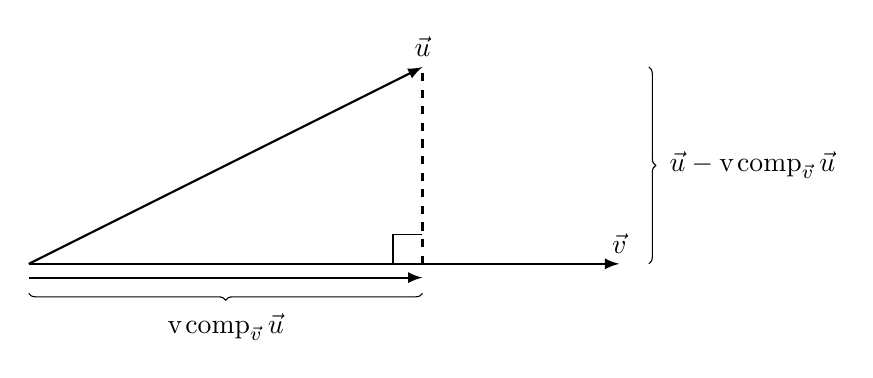
\begin{tikzpicture}[>=latex, scale=2.5]
			\draw[->,thick,black] (0,0) -- (2,1) node [above]
				{$\vec u$};

			\draw[->,thick,black] (0,0) -- (3,0) node [above]
				{$\vec v$};

			\draw[->,thick,black,yshift=-.07cm] (0,0) -- (2,0);
			\draw[decoration={brace, mirror}, decorate, yshift=-.15cm]
				(0,0) -- (2,0) node [midway,below,yshift=-4pt] {$\Comp_{\vec
				v}\vec u$};

			\draw[dashed,thick,black] (2,0) -- (2,1);
			\draw[decoration={brace, mirror}, decorate, xshift=1.15cm]
				(2,0) -- (2,1) node [midway,right,xshift=4pt]
				{$\vec u-\Comp_{\vec v}\vec u$};

			\draw[thin,black] (1.85,0)--(1.85,.15)--(2,.15);
		\end{tikzpicture}
	\end{center}
\end{SaveDefinition}

\begin{SaveDefinition}[key=Subspace, title={Subspace}]
	A non-empty subset $V\subseteq \R^{n}$ is called a \emph{subspace}\index{Subspace}\index[definitions]{Subspaces} if for all $\vec u,\vec v\in V$ and all
	scalars $k$ we have
	\begin{enumerate}
		\item[(i)] $\vec u+\vec v\in V$; and

		\item[(ii)] $k\vec u\in V$.
	\end{enumerate}
\end{SaveDefinition}

\begin{SaveDefinition}[key=TrivialSubspace, title={Trivial Subspace}]
	The subset $\Set{\vec 0}\subseteq\R^n$ is called the \emph{trivial subspace}\index{Subspace!trivial subspace}\index[definitions]{Subspace!trivial subspace}.
\end{SaveDefinition}

\begin{SaveDefinition}[key=Basis, title={Basis}]
	A
	\emph{basis}\index[definitions]{Basis}\index{Basis} for a subspace $\mathcal V$ is a linearly independent set of vectors,
	$\mathcal B$, so that $\Span\mathcal B=\mathcal V$.
\end{SaveDefinition}

\begin{SaveDefinition}[key=Dimension, title={Dimension}]
	The
	\emph{dimension}\index[definitions]{Subspace!dimension}\index{Subspace!dimension} of a subspace $V$ is the number of elements in a basis
	for $V$.
\end{SaveDefinition}

\begin{SaveDefinition}[key=StandardBasisforRn, title={Standard Basis}]
	The \emph{standard basis}\index[definitions]{Basis!standard basis}\index{Basis!standard basis} for $\R^n$ is the set $\Set{\vec e_1,\ldots,\vec e_n}$ where
	\[
		\vec e_1=\matc{1\\0\\0\\\vdots}\qquad
		\vec e_2=\matc{0\\1\\0\\\vdots}\qquad
		\vec e_3=\matc{0\\0\\1\\\vdots}\qquad\cdots.
	\]
	That is $\vec e_i$ is the vector with a $1$ in its
	$i$th coordinate and zeros elsewhere.
\end{SaveDefinition}

\begin{SaveDefinition}[
	key=RepresentationinaBasis,
	title={Representation in a Basis}]

	Let $\mathcal B=\Set{\vec b_1,\ldots,\vec b_n}$ be a basis for a
	subspace $V$ and let $\vec v\in V$. The
	\emph{representation of $\vec v$ in the $\mathcal B$ basis}\index{Vector!representation in a basis}\index[definitions]{Vector!representation in a basis}, notated $[\vec
	v]_{\mathcal B}$\index[symbols]{$[\vec v]_{\mathcal B}$}, is the column matrix
	\[
		[\vec v]_{\mathcal B}= \matc{\alpha_1\\\vdots\\\alpha_n}
	\]
	 where $\alpha_{1},\ldots,\alpha_{n}$ uniquely satisfy
	$\vec v=\alpha_{1}\vec b_{1}+\cdots+\alpha_{n}\vec b_{n}.$

	Conversely,
	\[
		\matc{\alpha_1\\\vdots\\\alpha_n}_{\mathcal B}= \alpha_{1}\vec b_{1}+\cdots
		+\alpha_{n}\vec b_{n}
	\]
	 is notation for the linear combination of $\vec b_{1},\ldots,\vec b_{n}$
	with coefficients $\alpha_{1},\ldots,\alpha_{n}$.
\end{SaveDefinition}

\begin{SaveDefinition}[key=OrthonormalBasis, title={Orthonormal Basis}]
	A basis $\mathcal B=\{\vec b_{1},\ldots,\vec b_{n}\}$ is called
	\emph{orthonormal}\index[definitions]{Basis!orthonormal basis}\index{Basis!orthonormal basis} if every basis vector is a unit vector and all
	basis vectors are orthogonal to each other. That is,
	\[
		\vec b_i\cdot \vec b_j=\begin{cases}
			1 &\text{ if }\quad i=j\\
			0 &\text{ if }\quad i\neq j
		\end{cases}.
	\]
\end{SaveDefinition}

\begin{SaveDefinition}[key=OrientationofaBasis, title={Orientation of a Basis}]
	The ordered basis $\mathcal B=\{\vec b_{1},\ldots,\vec b_{n}\}$ is
	\emph{right-handed}\index[definitions]{Basis!right-handed}\index{Basis!right-handed} or
	\emph{positively oriented}\index[definitions]{Basis!positively oriented}\index{Basis!positively oriented} if it can be continuously transformed to the
	standard basis (with $\vec b_{i}\mapsto \vec e_{i}$) while remaining
	linearly independent throughout the transformation. Otherwise,
	$\mathcal B$ is called
	\emph{left-handed}\index[definitions]{Basis!left-handed}\index{Basis!left-handed} or
	\emph{negatively oriented}\index[definitions]{Basis!negatively oriented}\index{Basis!negatively oriented}.
\end{SaveDefinition}

\begin{SaveDefinition}[key=LinearTransformation, title={Linear Transformation}]
	Let $V$ and $W$ be subspaces. A function $T:V\to W$ is called a
	\emph{linear transformation}\index[definitions]{Linear transformation}\index{Linear transformation} if
	\[
		T(\vec u+\vec v)=T(\vec u)+T(\vec v) \qquad\text{and}\qquad T(\alpha
		\vec v)=\alpha T(\vec v)
	\]
	 for all vectors $\vec u,\vec v\in V$ and all scalars $\alpha$.
\end{SaveDefinition}

\begin{SaveDefinition}[key=ImageofaSet, title={Image of a Set}]
	Let $L:\R^n\to \R^m$ be a transformation and let $X\subseteq \R^n$ be a set. The
	\emph{image of the set $X$ under $L$}\index[definitions]{Set!image of}\index{Set!image of}, denoted $L(X)$\index[symbols]{$L(X)$ (Image of a set)}, is the set
	\[
		L(X)=\Set{\vec y\in \R^m \given \vec y=L(\vec x)\text{ for some }\vec
		x\in X}.
	\]
\end{SaveDefinition}

\begin{SaveDefinition}[key=CompositionofFunctions, title={Composition of Functions}]
	Let $f:A\to B$ and $g:B\to C$. The \emph{composition}\index[definitions]{Function!composition}\index{Function!composition} of $g$ and $f$, notated $g\circ f$\index[symbols]{$g\circ f$},
	is the function $h:A\to C$ defined by
	\[
		h(x)=g\circ f(x) = g\Big(f(x)\Big).
	\]
\end{SaveDefinition}

\begin{SaveDefinition}[key=Range, title={Range}]
	The
	\emph{range} (or
	\emph{image})\index[definitions]{Linear transformation!range (image)}\index{Linear transformation!range (image)} of a linear transformation $T:V\to W$ is the set of vectors
	that $T$ can output. That is,
	\[
		\Range(T)=\Set{\vec y\in W \given \vec y=T\vec x\text{ for some }\vec
		x\in V}.
	\]

\end{SaveDefinition}

\begin{SaveDefinition}[key=NullSpace, title={Null Space}]
	The
	\emph{null space} (or
	\emph{kernel})\index[definitions]{Linear transformation!null space (kernel)}\index{Linear transformations!null space (kernel)} of a linear transformation $T:V\to W$ is the set of vectors
	that get mapped to the zero vector under $T$. That is,
	\[
		\Null(T)=\Set{\vec x\in V \given T\vec x=\vec 0}.
	\]

\end{SaveDefinition}

\begin{SaveDefinition}[
	key=InducedTransformation,
	title={Induced Transformation}]

	Let $M$ be an $n\times m$ matrix. We say $M$
	\emph{induces}\index[definitions]{Matrix!linear transformation induced by}\index{Matrix!linear transformation induced by}\index[definitions]{Linear transformation!induced}\index{Linear transformation!induced} a linear transformation $\mathcal T_{M}:\R^{m}\to\R^{n}$ defined
	by
	\[
		[\mathcal T_{M}\vec v]_{\mathcal E'}= M[\vec v]_{\mathcal E},
	\]
	 where $\mathcal E$ is the standard basis for $\R^{m}$ and $\mathcal E'$
	is the standard basis for $\R^{n}$.
\end{SaveDefinition}

\begin{SaveDefinition}[
	key=Transpose,
	title={Transpose}]

	Let $M$ be an $n\times m$ matrix defined by
	\[
		M=\matc{
			a_{11}&a_{12}&a_{13}&\cdots & a_{1m}\\
		a_{21}&a_{22}&a_{23}&\cdots&a_{2m}\\
		\vdots &\vdots&\vdots &\ddots&\vdots\\
		a_{n1}&a_{n2}&a_{n3}&\cdots&a_{nm}}.
	\]
	The \emph{transpose}\index[definitions]{Matrix!transpose of}\index{Matrix!transpose of} of $M$, notated $M^T$\index[symbols]{$M^T$}, is the $m\times n$ matrix produced by swapping the rows
	and columns of $M$. That is
	\[
		M^T=\matc{
		a_{11}&a_{21}&\cdots&a_{n1}\\
		a_{12}&a_{22}&\cdots&a_{n2}\\
		a_{13}&a_{23}&\cdots&a_{n3}\\
		\vdots&\vdots&\ddots&\vdots\\
		a_{1m}&a_{2m}&\cdots&a_{nm}}.
	\]
\end{SaveDefinition}

\begin{SaveDefinition}[
	key=ElementaryMatrix,
	title={Elementary Matrix}]

	A matrix is called an \emph{elementary matrix}\index[definitions]{Matrix!elementary matrix}\index{Matrix!elementary matrix} if it is an identity matrix with a single elementary row operation applied.
\end{SaveDefinition}

\begin{SaveDefinition}[
	key=MatrixInverse,
	title={Matrix Inverse}]

	The \emph{inverse}\index[definitions]{Matrix!inverse of}\index{Matrix!inverse of} of a matrix $A$ is a
		matrix $B$ such that $AB=I$ and $BA=I$.
		In this case, $B$ is called the inverse of $A$ and is notated $A^{-1}$.
\end{SaveDefinition}

\begin{SaveDefinition}[
	key=IdentityFunction,
	title={Identity Function}]

	Let $X$ be a set. The \emph{identity function}\index[definitions]{Function!identity function}\index{Function!identity function} with domain and codomain $X$,
	notated $\Ident:X\to X$\index[symbols]{$\Ident$}, is the function satisfying
	\[
		\Ident(x)=x
	\]
	for all $x\in X$.
\end{SaveDefinition}

\begin{SaveDefinition}[
	key=InverseFunction,
	title={Inverse Function}]

	Let $f:X\to Y$ be a function. We say $f$ is \emph{invertible}\index[definitions]{Function!invertible function}\index{Function!invertible function} if
	there exists a function $g:Y\to X$ so that $f\circ g=\Ident$ and $g\circ f=\Ident$.
	In this case, we call $g$ an \emph{inverse}\index[definitions]{Function!inverse of}\index{Function!inverse of} of $f$ and write
	\[
		f^{-1}=g.
	\]
\end{SaveDefinition}

\begin{SaveDefinition}[
	key=Onetoone,
	title={One-to-one}]

	Let $f:X\to Y$ be a function. We say $f$ is \emph{one-to-one}\index[definitions]{One-to-one function}\index{One-to-one function} (or \emph{injective}\index{Injective function}\index[definitions]{Injective function}) if
	distinct inputs to $f$ produce distinct outputs. That is $f(x)=f(y)$ implies $x=y$.
\end{SaveDefinition}

\begin{SaveDefinition}[
	key=Onto,
	title={Onto}]

	Let $f:X\to Y$ be a function.
	We say $f$ is \emph{onto}\index{Onto function}\index[definitions]{Onto function} (or \emph{surjective}\index{Surjective function}\index[definitions]{Surjective function}) if every point in the codomain of $f$ gets mapped to.
	That is $\Range(f)=Y$.
\end{SaveDefinition}

\begin{SaveDefinition}[
	key=IdentityMatrix,
	title={Identity Matrix}]

	An \emph{identity matrix}\index{Matrix!identity matrix}\index[definitions]{Matrix!identity matrix} is a square matrix with ones on the diagonal
	and zeros everywhere else. The $n\times n$ identity matrix is denoted $I_{n\times n}$,
	or just $I$ when its size is implied.
\end{SaveDefinition}

\begin{SaveDefinition}[key=FundamentalSubspaces, title={Fundamental Subspaces}]
	\index{Matrix!fundmamental subspaces of}\index[definitions]{Matrix!fundamental subspaces of}
	Associated with any matrix $M$ are three fundamental subspaces: the
	\emph{row space}\index{Matrix!row space}\index[definitions]{Matrix!row space} of $M$, denoted $\Row(M)$\index[symbols]{$\Row(M)$}, is the span of the rows of
	$M$; the
	\emph{column space}\index{Matrix!column space}\index[definitions]{Matrix!column space} of $M$, denoted $\Col(M)$\index[symbols]{$\Col(M)$}, is the span of the
	columns of $M$; and the
	\emph{null space}\index{Matrix!null space}\index[definitions]{Matrix!null space} of $M$, denoted $\Null(M)$\index[symbols]{$\Null(M)$}, is the set of solutions to
	$M\vec x=\vec 0$.
\end{SaveDefinition}

\begin{SaveDefinition}[key=RankofaLinearTransformation, title={Rank of a Linear Transformation}]
	For a linear transformation $T:\R^n\to \R^m$, the
	\emph{rank}\index[definitions]{Linear transformation!rank}\index{Linear transformation!rank} of $T$, denoted $\Rank(T)$\index[symbols]{$\Rank(T)$}, is the dimension of the range of
	$T$.
\end{SaveDefinition}

\begin{SaveDefinition}[key=RankofaMatrix, title={Rank of a Matrix}]
	Let $M$ be a matrix.
	The \emph{rank}\index[definitions]{Matrix!rank}\index{Matrix!rank} of $M$, denoted $\Rank(M)$\index[symbols]{$\Rank(M)$}, is the rank of
	the linear transformation induced by $M$.
\end{SaveDefinition}

\begin{SaveDefinition}[key=NullityofaMatrix, title={Nullity of a Matrix}]
	Let $M$ be a matrix.
	The \emph{nullity}\index[definitions]{Matrix!nullity}\index{Matrix!nullity} of $M$, denoted $\Nullity(M)$\index[symbols]{$\Nullity(M)$}, is the nullity of
	the linear transformation induced by $M$.
\end{SaveDefinition}

\begin{SaveDefinition}[key=Rank, title={Rank}]
	For a linear transformation $T:\R^n\to \R^m$, the
	\emph{rank} of $T$, denoted $\Rank(T)$, is the dimension of the range of
	$T$.\index[definitions]{Linear transformation!rank}\index{Linear transformation!rank}

	For an $m\times n$ matrix $M$, the
	\emph{rank} of $M$, denoted $\Rank(M)$, is the dimension of the 
	column space of $M$.\index[definitions]{Matrix!nullity}\index{Matrix!nullity}
\end{SaveDefinition}

\begin{SaveDefinition}[key=Nullity, title={Nullity}]
	For a linear transformation $T:\R^n\to \R^m$, the
	\emph{nullity} of $T$, denoted $\Nullity(T)$, is the dimension of the null space of
	$T$.\index[definitions]{Linear transformation!nullity}\index{Linear transformation!nullity}
\end{SaveDefinition}

\begin{SaveDefinition}[key=ChangeofBasisMatrix, title={Change of Basis Matrix}]
	Let $\mathcal A$ and $\mathcal B$ be bases for $\R^n$. The matrix $M$ is called
	a \emph{change of basis} matrix\index[definition]{Change of basis matrix}\index{Change of basis matrix} (which converts from $\mathcal A$ to $\mathcal B$) if
	for all $\vec x\in \R^n$
	\[
		M[\vec x]_{\mathcal A}=[\vec x]_{\mathcal B}.
	\]
	 Notationally, $\BasisChange{\mathcal A}{\mathcal B}$\index[symbols]{$\protect\BasisChange{\mathcal A}{\mathcal B}$}
	stands for the change of basis matrix converting from $\mathcal A$ to $\mathcal B$,
	and we may write $M=\BasisChange{\mathcal A}{\mathcal B}$.
\end{SaveDefinition}

\begin{SaveDefinition}[key=LinearTransformationinaBasis, title={Linear Transformation in a Basis}]
	Let $\mathcal T:\R^n\to\R^n$ be a linear transformation and let $\mathcal B$ be a
	basis for $\R^n$. The \emph{matrix for $\mathcal T$ with respect to $\mathcal B$}, notated
	$[\mathcal T]_{\mathcal B}$,
	is the $n\times n$ matrix satisfying
	\[
		[\mathcal T\vec x]_{\mathcal B} = [\mathcal T]_{\mathcal B}[\vec x]_{\mathcal B}.
	\]
	In this case, we say the matrix $[\mathcal T]_{\mathcal B}$\index[symbols]{$[\mathcal T]_{\mathcal B}$} is the representation
	of $\mathcal T$ in the $\mathcal B$ basis.
	\index{Matrix!of a linear transformation}\index[definitions]{Matrix!of a linear transformation}\index{Linear transformation!representation in a basis}\index[definitions]{Linear transformation!representation in a basis}
\end{SaveDefinition}

\begin{SaveDefinition}[key=SimilarMatrices, title={Similar Matrices}]
	The matrices $A$ and $B$ are called
	\emph{similar matrices}\index[definitions]{Matrix!similar matrices},
	denoted $A\sim B$\index[symbols]{$\sim$}, if $A$ and $B$ represent the
	same linear transformation but in possibly different bases. Equivalently,
	$A\sim B$ if there is an invertible matrix $X$ so that
	\[
		A=XBX^{-1}.
	\]

\end{SaveDefinition}

\begin{SaveDefinition}[key=Unitncube, title={Unit $n$-cube}]
	The
	\emph{unit $n$-cube}\index[definitions]{Unit $n$-cube ($C_n$)}\index{Unit $n$-cube ($C_n$)} is the $n$-dimensional cube with sides given by the
	standard basis vectors and lower-left corner located at the origin. That
	is
	\[
		C_{n}=\Set*{\vec x\in\R^n:\vec x=\sum_{i=1}^n\alpha_i\vec e_i\text{
		for some }\alpha_1,\ldots,\alpha_n\in[0,1]}=[0,1]^{n}.
	\]\index[symbols]{$C_n$}

\end{SaveDefinition}

\begin{SaveDefinition}[key=Determinant, title={Determinant}]
	The
	\emph{determinant}\index{Determinant}\index[definitions]{Determinant} of a linear transformation $\mathcal T:\R^{n}\to \R^{n}$, denoted $\det(\mathcal T)$\index[symbols]{$\det(\mathcal T)$} or $\Abs{\mathcal T}$\index[symbols]{$\Abs{\mathcal T}$}, is
	the oriented volume of the image of the unit $n$-cube. The determinant of
	a square matrix is the determinant of its induced transformation.
\end{SaveDefinition}

\begin{SaveDefinition}[key=OrientationPreservingLinearTransformation, title={Orientation Preserving Linear Transformation}]
	Let $\mathcal T:\R^n\to\R^n$ be a linear transformation. We say $\mathcal T$
	is \emph{orientation preserving}\index[definitions]{Linear transformation!orientation preserving}\index{Linear transformation!orientation preserving} if the ordered basis $\Set{\mathcal T(\vec e_1),\ldots, \mathcal T(\vec e_n)}$
	is positively oriented  and we say $\mathcal T$
	is \emph{orientation reversing}\index[definitions]{Linear transformation!orientation reversing}\index{Linear transformation!orientation reversing} if the ordered basis $\Set{\mathcal T(\vec e_1),\ldots, \mathcal T(\vec e_n)}$
	is negatively oriented. If $\Set{\mathcal T(\vec e_1),\ldots, \mathcal T(\vec e_n)}$
	is not a basis for $\R^n$, then $\mathcal T$ is neither orientation preserving nor orientation reversing.
\end{SaveDefinition}

\begin{SaveDefinition}[key=Eigenvector, title={Eigenvector}]
	Let $X$ be a linear transformation or a matrix. An
	\emph{eigenvector}\index[definitions]{Eigenvector}\index{Eigenvector} for $X$ is a non-zero vector that doesn't change
	directions when $X$ is applied. That is, $\vec v\neq \vec 0$ is an
	eigenvector for $X$ if
	\[
		X\vec v=\lambda \vec v
	\]
	 for some scalar $\lambda$. We call $\lambda$ the
	\emph{eigenvalue}\index[definitions]{Eigenvalue}\index{Eigenvalue} of $X$ corresponding to the eigenvector $\vec v$.
\end{SaveDefinition}

\begin{SaveDefinition}[
	key=CharacteristicPolynomial,
	title={Characteristic Polynomial}]

	For a matrix $A$, the
	\emph{characteristic polynomial}\index{Characteristic polynomial}\index[definition]{Characteristic Polynomial} of $A$ is
	\[
		\chr(A)=\det(A-\lambda I).
	\]\index[symbols]{$\chr(A)$}

\end{SaveDefinition}

\begin{SaveDefinition}[key=Diagonalizable, title={Diagonalizable}]
	A matrix is
	\emph{diagonalizable}\index{Matrix!diagonalizable}\index[definitions]{Matrix!diagonalizible} if it is similar to a diagonal matrix.
\end{SaveDefinition}

\begin{SaveDefinition}[key=Eigenspace, title={Eigenspace}]
	Let $A$ be an $n\times n$ matrix with eigenvalues
	$\lambda_{1},\ldots,\lambda_{m}$. The
	\emph{eigenspace}\index[definitions]{Eigenspace}\index{Eigenspace} of $A$ corresponding to the eigenvalue $\lambda_{i}$
	is the null space of $A-\lambda_{i} I$. That is, it is the space spanned
	by all eigenvectors that have the eigenvalue $\lambda_{i}$.

	The
	\emph{geometric multiplicity}\index[definitions]{Eigenvalue!geometric multiplicity}\index{Eigenvalue!geometric multiplicity} of an eigenvalue $\lambda_{i}$ is the
	dimension of the corresponding eigenspace. The
	\emph{algebraic multiplicity}\index[definitions]{Eigenvalue!algebraic multiplicity}\index{Eigenvalue!algebraic multiplicity} of $\lambda_{i}$ is the number of times
	$\lambda_{i}$ occurs as a root of the characteristic polynomial of $A$ (i.e.,
	the number of times $x-\lambda_{i}$ occurs as a factor).
\end{SaveDefinition}


\begin{SaveDefinition}[key=Diagonal, title={Diagonal}]
	The \emph{diagonal}\index[definitions]{Matrix!diagonal of} of an $m\times n$ matrix $A=[a_{ij}]$ consists of
	the entries $a_{ij}$ satisfying $i=j$.
\end{SaveDefinition}
\begin{SaveDefinition}[key=SquareMatrix, title={Square Matrix}]
	A matrix is called \emph{square}\index[definitions]{Matrix!square} if it has the same
	number of rows as columns.
\end{SaveDefinition}
\begin{SaveDefinition}[key=DiagonalMatrix, title={Diagonal Matrix}]
	A square matrix is called \emph{diagonal}\index[definitions]{Matrix!diagonal} the only non-zero
	entries in the matrix appear on the diagonal.
\end{SaveDefinition}
\begin{SaveDefinition}[key=TriangleOf, title={Upper \& Lower Triangle}]
	Let $A=[a_{ij}]$ be an $m\times n$ matrix. The \emph{upper triangle}\index[definitions]{Matrix!upper triangle of}
	of $A$ consists the entries $a_{ij}$
	satisfying $j\geq i$. The \emph{lower triangle}\index[definitions]{Matrix!lower triangle of}
	of $A$ consists of the entries $a_{ij}$ satisfying $j\leq i$.
\end{SaveDefinition}
\begin{SaveDefinition}[key=TriangularMatrix, title={Triangular Matrices}]
	A matrix is called \emph{upper triangular}\index[definitions]{Matrix!upper triangular} if all non-zero entries lie in the upper triangle of the matrix and
	a matrix is called \emph{lower triangular}\index[definitions]{Matrix!lower triangular} if all non-zero entries lie in the lower triangle. A matrix is
	called \emph{triangular}\index[definitions]{Matrix!triangular} if it is either upper or lower triangular.
\end{SaveDefinition}
\begin{SaveDefinition}[key=SymmetricMatrix, title={Symmetric Matrix}]
	The square matrix $A=[a_{ij}]$ is called \emph{symmetric}\index[definitions]{Matrix!symmetric} if its
	entries satisfy $a_{ij}=a_{ji}$.

	Alternatively, if the entries of $A$ satisfy $a_{ij}=-a_{ji}$, then $A$
	is called \emph{skew-symmetric} or \emph{anti-symmetric}\index[definitions]{Matrix!skew-symmetric}.
\end{SaveDefinition}
\begin{SaveDefinition}[key=ZeroMatrix, title={Zero Matrix}]
	A matrix is called a \emph{zero matrix}\index[definitions]{Matrix!zero matrix} if all its entries are zero.
\end{SaveDefinition}



%%
%% End Definitions
%%

%\begin{module}
%	\Title{Systems of Linear Equations}
%
%		An \emph{equation} encodes a relationship between quantities. For
	example, writing
	\[
		\underbrace{\text{Slices of cake}}_C = \underbrace{\text{Slices you ate}}_M + \underbrace{\text{Slices your brother ate}}_B
	\]
	specifies a precise relationship between the quantities $C$, $M$, and $B$. 
	Without more information, $C$, $M$, and $B$ could be almost anything. As such, we call 
	$C$, $M$, and $B$
	\emph{variables} or \emph{unknowns}. 
	However, the
	relationship \emph{between} them is precisely defined. 

	Additional relationships give rise to additional equations, which we express concisely as a
	\emph{system of equations}, that is, a list of equations. For example, suppose you know the cake
	had six pieces and your brother ate twice as many pieces as you. We might now write the system
	\[
		\sysdelim..
		\systeme{C=M+B,B=2M,C=6}
	\]
	which should be interpreted as: ``the relationship $C=M+B$ holds \emph{and} the relationship $B=2M$ holds \emph{and}
	the relationship $C=6$ holds.''
	All this information, taken together, is enough to deduce the unknowns: $M=2$, $B=4$, and $C=6$.

	Systems of equations naturally appear in linear algebra through vector equations. Suppose $\vec u=\mat{1\\2}$, $\vec v=\mat{2\\3}$,
	and $\vec w=\mat{1\\1}$. You might wonder if $\vec w$ was a linear combination of $\vec u$ and $\vec v$. The answer is \emph{yes} if and
	only if the vector equation
	\[
		\vec w=a\vec u+b\vec v
	\]
	has a solution for some $a$ and $b$. Written in coordinates, this equation is equivalent to
	\[
		\mat{1\\1}=a\mat{1\\2}+b\mat{2\\3} = \mat{a+2b\\2a+3b}.
	\]
	Equating coordinates, a system of equations appears:
	\[
		\systeme{a+2b=1,2a+3b=1}
	\]

	Every vector equation, by way of coordinates, corresponds to a system of equations. And, fortunately for us, there is
	an \emph{algorithm} to find all solutions to these systems\footnote{ Saying there is an \emph{algorithm} for ``$X$''
	means that there is a specific set of (non-random) rules that \emph{always} accomplishes ``$X$''. As a consequence, doing
	``$X$'' never requires special insight. For example, there \emph{is} an algorithm for multiplying numbers, but there \emph{is not}
	an algorithm for factoring polynomials of degree 5 or greater.}.

	\Heading{Systems of Linear Equations}

	There's no guarantee that a general equation, like $x^4-e^x+7=0$, has a solution, and it might
	be impossible to decide if an arbitrary equation has a solution, let alone what the solutions 
	are!\footnote{ Fermat's Last Theorem famously claimed that $a^n+b^n=c^n$
	has no positive integer solutions for $n\geq 3$. However, it took 350 years of human ingenuity before anyone was able rigorously
	back up the claim.} However, for \emph{linear} equations and systems of linear equations we can \emph{always} tell
	whether there is a solution and what the solution(s) are.
	
	\begin{definition}[Linear Equation]
		A \emph{linear equation} in the variables $x_1,\ldots,x_n$ is one that can be expressed
		as
		\[
			a_1x_1+a_2x_2+\cdots+a_nx_n=c
		\]
		for constants $a_1,\ldots, a_n$ and $c$. A \emph{system of linear equations} is a system of equations 
		consisting of one or more linear equations.
	\end{definition}

	Every vector equation corresponds to an \emph{equivalent} system of linear equations and vice versa, where equivalent
	means ``expresses the same relationships between variables''.

	\begin{example}
		Write down the vector equation corresponding to the system of linear equations $\systeme{2x+3y+z=2,y-z=-1}$
		and the system of linear equations corresponding to the vector equation $t\vec w+\vec u=r\vec v$ where $\vec w=\mat{1\\-1}$, $\vec u=\mat{2\\3}$,
		and $\vec v=\mat{4\\4}$.

		The system $\systeme{2x+3y+z=2,0x+y-z=-1}$ corresponds to the vector equation
		\[
			x\mat{2\\0} + y\mat{3\\1} + z\mat{1\\-1} = \mat{2\\-1}.
		\]
		
		As for the vector equation $t\vec w+\vec u=r\vec v$, rewriting each vector in coordinates gives us a corresponding system of linear equations:
		\begin{align*}
			t\vec w + \vec u = r\vec v
			\rightarrow
			t\mat{1\\-1} + \mat{2\\3} &= r\mat{4\\4}\\
			\mat{t+2\\-t+3} &= \mat{4r\\4r}
			\rightarrow
			\systeme{t-4r=-2, -t-4r=-3}.
		\end{align*}
	\end{example}

	\begin{emphbox}[Takeaway]
		Every vector equation corresponds to a system of linear equations and every system of linear equations
		corresponds to a vector equation.
	\end{emphbox}

	\Heading{Solution Sets}

	Before looking at how to solve systems of linear equations, let's agree on some terminology.

	A \emph{solution} to an equation is a particular choice of values for the variables that satisfy (i.e. make true)
	the equation. For example
	\begin{equation}
		\label{SOLNSETEXAMPLE}
		x+y=4
	\end{equation}
	has a solution $x=y=2$. However, $x=y=2$ is just one of \emph{many} possible solutions; we also have $x=4$ and $y=0$ or $x=-2$ and
	$y=6$. The \emph{solution set},
	also called the \emph{complete solution}, to an equation (or system of equations) is the set of all possible solutions.
	For example, the solution set to Equation \eqref{SOLNSETEXAMPLE} is $S=\Set{(x,y)\given y=4-x}$. %=\Set{(t,4-t)\given a\in \R}$.
	In this case, $S$ contains infinitely many solutions, including $(x,y)=(2,2)$, the first solution we found.

	Solution sets look a lot like sets of vectors: the set $S=\Set{(x,y)\given y=4-x}$ could be thought of as a subset of $\R^2$
	where we identify a solution $x=a$ and $y=b$ with the column vector $\mat{a\\b}$. Drawing $S$ as a subset of $\R^2$, we see a familiar
	picture.

	\begin{center}
		\begin{tikzpicture}
			\begin{axis}[
				anchor=origin,
				disabledatascaling,
				xmin=0,xmax=5,
				ymin=0,ymax=5,
				xtick={-1,...,5},
				ytick={-1,...,5},
				x=1cm,y=1cm,
				grid=both,
				grid style={line width=.1pt, draw=gray!10},
				axis lines=middle,
				minor tick num=0,
				enlargelimits={abs=0.5},
				axis line style={latex-latex},
				ticklabel style={font=\tiny,fill=white},
				xlabel style={at={(ticklabel* cs:1)},anchor=north west},
				ylabel style={at={(ticklabel* cs:1)},anchor=south west}
			]
				\draw [mygreen, thick] (-2,6) -- (6,-2);
			\end{axis}
		\end{tikzpicture}
	\end{center}

	It's the graph of the line given in $y=mx+b$ form by $y=-x+4$. In other words, \emph{via solution sets, equations and systems
	of equations can represent geometric objects.}

%	\medskip
%	If this all seems straightforward, great! Since grade school you've been training to apply algebra to geometry problems
%	and vice versa\footnote{ It was a big deal when equations saw their first applications to geometry and it is by no means
%	an obvious idea! If you're interested, look up the history of \emph{analytic geometry}, which is the formal name for what
%	we're doing.}. However, we need to take special care to note the assumptions we've made. After all, it would be
%	perfectly reasonable to claim that $S'=\Set{(y,x)\given y=4-x}$ (note the difference between $S$ and $S'$) 
%	is the solution set to Equation \eqref{SOLNSETEXAMPLE}.
%	However, it becomes less clear how $S'$ should be interpreted as a subset of $\R^2$. Should $(y,x)=(a,b)$ correspond to the
%	column vector $\mat{a\\b}$ or is $\mat{b\\a}$ the correct column vector? To solve this issue, we use the following convention.
%
%	\begin{emphbox}[Solution Set Convention] Unless otherwise specified,
%		solutions are converted to column vectors based on the order the variables are specified
%		in the original equations. This order will almost always be alphabetical if variables are assigned
%		different letters (e.g, $x$, $y$, $z$) or numerically if variables are indexed (e.g., $x_1$, $x_2$, $x_3$).
%	\end{emphbox}
%
%	Following this convention, $S$ is the ``correct'' solution set. That is, without specifying otherwise, the solutions
%	to $x+y=4$ correspond to the set $\Set*{\mat{a\\b}\given b=4-a}\subseteq \R^2$. This just so happens to agree with grade-school
%	convention\footnote{ It's as if there's a vast underworld of educators who plan how math should be taught from the time you
%	were five up until now.}.

	\Heading{Consistent \& Inconsistent Systems}

	Consider the following equations (as separate equations, not as a system):
	\[
		x^2=0\qquad\text{with solution set}\qquad S_x\subseteq \R,
	\]
	\[
		y^2=4\qquad\text{with solution set}\qquad S_y\subseteq \R,
	\]
	and
	\[
		z^2=-1\qquad\text{with solution set}\qquad S_z\subseteq \R.
	\]
	$S_x=\Set{0}$ consists of a single number. $S_y=\Set{2,-2}$ consists of two numbers, and $S_z=\Set{}$ consists of no
	numbers\footnote{ We're not allowing complex numbers at the moment.}.
	In this case, we would call the first two equations \emph{consistent} and the third equation \emph{inconsistent}.

	\begin{definition}[Consistent \& Inconsistent]
		An equation or system of equations is called \emph{consistent} if it has at least one solution. That
		is, its solution set is non-empty. Otherwise, an equation or system of equations is called \emph{inconsistent}.
	\end{definition}

	Why the word \emph{consistent}? This comes from the term \emph{logically consistent} which means ``able to be true''.
	An equation is an assertion that the left hand side equals the right hand side. If that can never happen, the assertion
	is not logically consistent.

	This terminology becomes more clear with systems. Consider the system
	\[
		\systeme{x-y=0,x-y=1}.
	\]
	From the first equation, we deduce $y=x$. From the second equation, we deduce $x=1+y$. Since $x=x$, we know that
	$y=x=1+y$ and therefore
	$y=1+y$. However, this is never true! There is a logical inconsistency between the two equations. In isolation they're
	fine, but taken together they're not.

	\Heading{Equivalent Systems}
	Two systems of equations are logically equivalent if they express the same relationships
	between their variables. For example, the equations $x=2y$ and $\tfrac{1}{2}x=y$ express the exact same
	relationship between the variables $x$ and $y$. This can be formalized using solution sets.

	\begin{definition}[Equivalent Systems]
		Two equations or systems of equations are called \emph{equivalent}\index[definitions]{Equivalent systems} if they have the same solution sets.
	\end{definition}

	Again, $x=2y$ and $\tfrac{1}{2}x=y$ both have the same solution set (a line through the origin of slope $\tfrac{1}{2}$),
	and so they are equivalent.

	Philosophical note: the process of ``doing algebra'' can be viewed as
	the process of \emph{manipulating equations/systems into easier to understand equivalent 
	equations/systems}. When you're asked to algebraically solve $x^2-4=0$. You might first factor to get the 
	equivalent equation $(x-2)(x+2)=0$. Then, since non-zero numbers cannot multiply to give zero, we know
	$x-2=0$ or $x+2=0$, which in turn is equivalent to $x=\pm2$. It's always been about equivalent systems!\footnote{
	Technically, up to this point we've been talking about \emph{conjunctive} systems, which means that a solution
	must hold for all equations of a system. The system $x=\pm 2$ is a \emph{disjunctive} system, which means a solution
	only needs to hold for \emph{one} of the equations ($x=2$ or $x=-2$), but the idea is the same.}

	\Heading{Row Reduction}

	Consider the vector equation
	\[
		t\vec u+s\vec v+r\vec w = \vec p\qquad\text{where}\qquad \vec u=\mat{1\\2\\1},\ 
		\vec v=\mat{2\\1\\-4},\ \vec w=\mat{-2\\-5\\1},\ \vec p=\mat{-15\\-21\\18}.
	\]
	By expanding in terms of coordinates, we get an equivalent system of linear equations.
	\begin{equation}
		\label{EQVECEQ2}
		\systeme[tsr]{
			t+2s-2r=-15@\qquad\text{row}_1,
			2t+s-5r=-21@\qquad\text{row}_2,
			t-4s+r=18@\qquad\text{row}_3
		}
	\end{equation}

	The most general way to solve any system is by \emph{substitution}. For System 
	\eqref{EQVECEQ2}, we could solve the first equation for $t$, substitute the result in
	the remaining equations, solve the next equation for $s$, etc.. However,
	because System \eqref{EQVECEQ2} is a \emph{linear} system, there's an alternate
	method: \emph{row reduction}\footnote{
	Row reduction is sometimes referred to as \emph{Gaussian elimination},
	\emph{Gauss-Jordan elimination}, or just \emph{elimination}; though there are subtle differences between Gaussian
	and Gauss-Jordan elimination,
	they aren't important, and we'll refer to all similar methods as \emph{row reduction}.}.

	Study the following manipulations of System \eqref{EQVECEQ2} and convince yourself
	that each operation produces a system equivalent to the one it came from.
	\begin{align}
	\sysdelim\{.
		\systeme[tsr]{
			t+2s-2r=-15,
			2t+s-5r=-21,
			t-4s+r=18
		}
		&\xrightarrow{\text{row}_3\mapsto\text{row}_3-\text{row}_1}
	\sysdelim\{.
		\systeme[tsr]{
			t+2s-2r=-15,
			2t+s-5r=-21,
			-6s+3r=33
		}\nonumber\\[4pt]
		&\xrightarrow{\text{row}_2\mapsto\text{row}_2-2\text{row}_1}
	\sysdelim\{.
		\systeme[tsr]{
			t+2s-2r=-15,
			-3s-r=9,
			-6s+3r=33
		}\nonumber\\[4pt]
		&\xrightarrow{\text{row}_3\mapsto\text{row}_3-2\text{row}_2}
	\sysdelim\{.
		\systeme[tsr]{
			t+2s-2r=-15,
			-3s-r=9,
			  5r=15
		}\label{EQEQUIVSYS}
	\end{align}
	From the final system, System \eqref{EQEQUIVSYS}, it's easy to see that $r=3$.
	From there,
	we can substitute $r=3$ into the second row of System \eqref{EQEQUIVSYS}
	to find $s=-4$ and we can substitute both $r$ and $s$ into the first row of System \eqref{EQEQUIVSYS}
	to find $t=-1$.

	By adding and subtracting rows, we ``reduced'' the number of variables from some equations until
	they were easy to solve. As an added benefit, every system along the way to System \eqref{EQEQUIVSYS}
	was nicely organized and formatted. In fact, the systems are so well organized that we can
	save time by not writing the variables and keeping track of the numbers in an \emph{augmented matrix}\footnote{
		A \emph{matrix} is a box of numbers. An \emph{augmented matrix} is a matrix with
		extra information associated with it.
	}. That is, instead of writing
	\[
		\systeme[tsr]{
			t+2s-2r=-15,
			2t+s-5r=-21,
			t-4s+r=18
		}
	\]
	we will write
	\[
		\begin{bmatrix}[rrr|r]
			1&2&-2 & -15\\
			2&1&-5&-21\\
			1&-4&1&18
		\end{bmatrix}.
	\]
	We call the matrix an \emph{augmented matrix} to stress that it contains two types of information:
	the \emph{coefficients} of the variables $t$, $s$, and $r$ and the \emph{constants} on
	the right hand side of the equations. An (optional) vertical line
	separates the two types of numbers.


	Now, the process of row reduction looks like this:
	\begin{align*}
		{\footnotesize
		\systeme[tsr]{
			t+2s-2r=-15,
			2t+s-5r=-21,
			t-4s+r=18
		}
		} \rightarrow
		\begin{bmatrix}[rrr|r]
			1&2&-2 & -15\\
			2&1&-5&-21\\
			1&-4&1&18
		\end{bmatrix}
		&\xrightarrow{\text{row}_3\mapsto\text{row}_3-\text{row}_1}
		\begin{bmatrix}[rrr|r]
			1&2&-2 & -15\\
			2&1&-5&-21\\
			0&-6&3&33
		\end{bmatrix}\\
		&\xrightarrow{\text{row}_2\mapsto\text{row}_2-2\text{row}_1}
		\begin{bmatrix}[rrr|r]
			1&2&-2 & -15\\
			0&-3&-1&9\\
			0&-6&3&33
		\end{bmatrix}\\
		&\xrightarrow{\text{row}_3\mapsto\text{row}_3-2\text{row}_2}
		\begin{bmatrix}[rrr|r]
			1&2&-2 & -15\\
			0&-3&-1&9\\
			0&0&5&15
		\end{bmatrix}
		\rightarrow
		{\footnotesize
			\systeme[tsr]{
			t+2s-2r=-15,
			-3s-r=9,
			  5r=15
			}
		}
	\end{align*}

	The operations are identical, but we write augmented matrices instead of equations.

	\begin{emphbox}[Takeaway]
		Augmented matrices are a notational tool that makes the process of doing row reduction more efficient.
	\end{emphbox}

	\Heading{The Rules of Row Reduction}

	So far, we've been able to row reduce systems by adding a multiple of one row to another\footnote{ Technically, we subtracted, but
	that's just adding a negative.}, but to fully solve \emph{any} system, we need additional operations\footnote{ If you're clever,
	you can think up alternatives to the elementary row operations that work just as well, but there's good reason to favor 
	the
	three elementary row operations. We'll see them when discussing matrix decompositions.}.
	\begin{definition}[Elementary Row Operations]
		The three \emph{elementary row operations}, which can be performed on a matrix or system of equations, are
		\smallskip
		\begin{itemize}
			\item swapping two rows (written $\text{row}_i\leftrightarrow \text{row}_j$),
			\item multiplying a row by a non-zero scalar (written $\text{row}_i\mapsto k\,\text{row}_i$), and
			\item adding a multiple of one row to another (written $\text{row}_i\mapsto \text{row}_i+ k\,\text{row}_j$).
		\end{itemize}
	\end{definition}

	Notice that each elementary row operation can be undone. For example, if you perform $\text{row}_i\mapsto k\,\text{row}_i$,
	you can undo it with $\text{row}_i\mapsto \tfrac{1}{k}\,\text{row}_i$. Therefore, applying an elementary row operation
	to a system is guaranteed to
	produce an equivalent system. 

	The strategy for solving a system is now summarized as:
	\begin{enumerate}
		\item Rewrite the system as an augmented matrix.
		\item Use elementary row operations to zero-out the lower triangle of the augmented matrix.
		\item Convert the matrix back to a system of equations.
		\item Read off the solution (substituting when necessary).
	\end{enumerate}

	\begin{example}
		Find a solution to the following system:
		\[
			\systeme{
				a+3b+2c=1,
				2a+7b+5c=2,
				-a-4b=11
			}.
		\]

		To do so, we rewrite the system as an augmented matrix then row reduce.
		\begin{align*}
			{\footnotesize
			\systeme{
				a+3b+2c=1,
				2a+7b+5c=2,
				-a-4b=11
			}
			} \rightarrow
			\begin{bmatrix}[rrr|r]
				1&3&2 & 1\\
				2&7&5 & 2\\
				-1&-4&0 & 11
			\end{bmatrix}
			&\xrightarrow{\text{row}_2\mapsto\text{row}_2-2\text{row}_1}
			\begin{bmatrix}[rrr|r]
				1&3&2 & 1\\
				0&1&1 & 0\\
				-1&-4&0 & 11
			\end{bmatrix}\\
			&\xrightarrow{\text{row}_3\mapsto\text{row}_3+\text{row}_1+\text{row}_2}
			\begin{bmatrix}[rrr|r]
				1&3&2 & 1\\
				0&1&1 & 0\\
				0&0&3 & 12
			\end{bmatrix}
			\rightarrow
			{\footnotesize
				\systeme{
				a+3b+2c=1,
				b+c=0,
				3c=12
				}
			}
		\end{align*}
		The third row reveals that $c=4$; substituting into the second row, we find $b=-4$. Now we can substitute $b=-4$ and $c=4$ into the first row and we obtain $a=5$.
		
		Thus, the solution is $\mat{a\\b\\c}=\mat{5\\-4\\4}$. Since this is the only solution to the system, the solution set is $\Set*{\mat{5\\-4\\4}}$.
	\end{example}

	\begin{example}
		Solve the system
		\[
			\systeme[tsr]{
				3t+s+13r=-2,
				t+5r=1,
				-t+s-6r=-8,
				t+s+4r=-6
			}.
		\]

		Again, we row reduce the corresponding augmented matrix to find an equivalent system\index{System of linear equations!equivalent} from which we can more easily compute the solution.
		\begin{align*}
			{\footnotesize
			\systeme[tsr]{
				3t+s+13r=-2,
				t+5r=1,
				-t+s-6r=-8,
				t+s+4r=-6
			}
			} \rightarrow
			\begin{bmatrix}[rrr|r]
				3&1&13 & -2\\
				1&0&5 & 1\\
				-1&1&-6 & -8\\
				1&1&4 & -6
			\end{bmatrix}
			&\xrightarrow{\text{row}_1\leftrightarrow\text{row}_2}
			\begin{bmatrix}[rrr|r]
				1&0&5 & 1\\
				3&1&13 & -2\\
				-1&1&-6 & -8\\
				1&1&4 & -6
			\end{bmatrix}\\
			&\xrightarrow{\text{row}_2\mapsto\text{row}_2-3\text{row}_1}
			\begin{bmatrix}[rrr|r]
				1&0&5 & 1\\
				0&1&-2 & -5\\
				-1&1&-6 & -8\\
				1&1&4 & -6
			\end{bmatrix}\\
			&\xrightarrow{\text{row}_3\mapsto\text{row}_3+\text{row}_1-\text{row}_2}
			\begin{bmatrix}[rrr|r]
				1&0&5 & 1\\
				0&1&-2 & -5\\
				0&0&1 & -2\\
				1&1&4 & -6
			\end{bmatrix}\\
			&\xrightarrow{\text{row}_4\mapsto\text{row}_4-\text{row}_1-\text{row}_2}
			\begin{bmatrix}[rrr|r]
				1&0&5 & 1\\
				0&1&-2 & -5\\
				0&0&1 & -2\\
				0&0&1 & -2
			\end{bmatrix}\\
			&\xrightarrow{\text{row}_4\mapsto\text{row}_4-\text{row}_3}
			\begin{bmatrix}[rrr|r]
				1&0&5 & 1\\
				0&1&-2 & -5\\
				0&0&1 & -2\\
				0&0&0 & 0
			\end{bmatrix}
			\rightarrow
			{\footnotesize
				\systeme[tsr]{
				t+5r=1,
				s-2r=-5,
				r=-2,
				0=0
				}
			}
		\end{align*}
		Our equivalent system reveals $r=-2$, which we can substitute back into the first and second rows to find that $t=11$ and $s=-9$.
		
		As a vector, the solution is $\mat{t\\s\\r}=\mat{11\\-9\\-2}$ and so the solution set is $\Set*{\mat{11\\-9\\-2}}$.
	\end{example}

	In the examples so far, we've stopped row reducing when the equations became simple enough
	to solve by inspection. However, we could continue row reducing until the system is as simple as possible.

	\begin{example}
		Solve the system
		\[
			\systeme{
				a+3b+2c=1,
				2a+7b+5c=2,
				-a-4b=11
			}
		\]

		Notice that we solved this system using a combination of row reduction and substitution in a previous example.
		This time, let us use only row reduction.
		
		The augmented matrix for this system is
		\[
			\begin{bmatrix}[rrr|r]
				1&3&2 & 1\\
				2&7&5 & 2\\
				-1&-4&0 & 11
			\end{bmatrix}.
		\]
		Based on the work from the previous example, we know it can be reduced to
		\[
			\begin{bmatrix}[rrr|r]
				1&3&2 & 1\\
				0&1&1 & 0\\
				0&0&3 & 12
			\end{bmatrix}.
		\]
		Now let us continue row reducing.
		\begin{align*}
			\begin{bmatrix}[rrr|r]
				1&3&2 & 1\\
				0&1&1 & 0\\
				0&0&3 & 12
			\end{bmatrix}
			&\xrightarrow{\text{row}_3\mapsto\tfrac{1}{3}\,\text{row}_3}
			\begin{bmatrix}[rrr|r]
				1&3&2 & 1\\
				0&1&1 & 0\\
				0&0&1 & 4
			\end{bmatrix}\\
			&\xrightarrow{\text{row}_2\mapsto\text{row}_2-\text{row}_3}
			\begin{bmatrix}[rrr|r]
				1&3&2 & 1\\
				0&1&0 & -4\\
				0&0&1 & 4
			\end{bmatrix}\\
			&\xrightarrow{\text{row}_1\mapsto\text{row}_1-3\text{row}_2-2\text{row}_3}
			\begin{bmatrix}[rrr|r]
				1&0&0 & 5\\
				0&1&0 & -4\\
				0&0&1 & 4
			\end{bmatrix}
			\rightarrow
			{\footnotesize
				\systeme{
				a=5,
				b=-4,
				c=4
				}
			}
		\end{align*}
		The solution is $\mat{a\\b\\c}=\mat{5\\-4\\4}$ and the solution set is $\Set*{\mat{5\\-4\\4}}$, which is the same as we got before.
	\end{example}

	What happens when you apply row reduction to an inconsistent system? Let's see. Consider the system
	\begin{equation}
		\label{EQSYSINCONEX}
		\systeme{x+y=1,4x+4y=7}.
	\end{equation}
	Before continuing, convince yourself that this system is inconsistent.
	The augmented matrix for System \eqref{EQSYSINCONEX} is
	\[
		\begin{bmatrix}[cc|c]1&1&1\\4&4&7\end{bmatrix}.
	\]
	We apply the row operation $\text{row}_2\mapsto \text{row}_2-4\text{row}_1$ to get
	\[
		\begin{bmatrix}[cc|c]1&1&1\\0&0&3\end{bmatrix},
	\]
	which corresponds to the system
	\[
		\systeme{x+y=1,0x+0y=3}.
	\]
	But, the last equation says $0x+0y=3$, which is not true for any choice of $x$ and $y$!
	Thus, we see applying row reduction to an inconsistent system reveals its inconsistency.

	\begin{example}
		Find a solution to the following system:
		\[
			\systeme{
				x+z=4,
				x+y+2z=-8,
				x+3y+4z=-18
			}.
		\]

		As usual we rewrite the system as an augmented matrix and then row reduce.
		\begin{align*}
			{\footnotesize
			\systeme{
				x+z=4,
				x+y+2z=-8,
				x+3y+4z=-18
			}
			} \rightarrow
			\begin{bmatrix}[rrr|r]
				1&0&1 & 4\\
				1&1&2 & -8\\
				1&3&4 & -18
			\end{bmatrix}
			&\xrightarrow{\text{row}_3\mapsto\text{row}_3-\text{row}_2}
			\begin{bmatrix}[rrr|r]
				1&0&1 & 4\\
				1&1&2 & -8\\
				0&2&2 & -10
			\end{bmatrix}\\
			&\xrightarrow{\text{row}_2\mapsto\text{row}_2-\text{row}_1}
			\begin{bmatrix}[rrr|r]
				1&0&1 & 4\\
				0&1&1 & -12\\
				0&2&2 & -10
			\end{bmatrix}\\
			&\xrightarrow{\text{row}_3\mapsto\text{row}_3-2\text{row}_2}
			\begin{bmatrix}[rrr|r]
				1&0&1 & 4\\
				0&1&1 & -12\\
				0&0&0 & 14
			\end{bmatrix}
			\rightarrow
			{\footnotesize
				\systeme{
				x+z=4,
				y+z=-12,
				0x+0y+0z=14
				}
			}
		\end{align*}
		The equation $0x + 0y + 0z = 14$ is never true and so the system is inconsistent.
		Since there are no values of $x$, $y$, and $z$ that satisfy the system, the solution set is $\Set*{}$, the empty set.
	\end{example}

%	\begin{exercises}
	\begin{problist}
		\prob For each equation given below, determine if it is a linear
		equation. If not, explain what makes it nonlinear.
		\begin{enumerate}
			\item $\cos(4)x_{1}+\mathrm{e}y_{2}+\pi z_{3}=\mathrm{e}^{\pi}$

			\item $4x_{1}+2x_{2}+5x_{4}=4x_{2}+4x_{5}+5$

			\item $5x+2y+8z=\cos(y)$

			\item $12x+3xy+5z=2$

			\item $\cos(4)x+\sin(4)y=\tan(4)x$

			\item $\frac{x}{y}=1$
		\end{enumerate}
		\begin{solution}
			\begin{enumerate}
				\item Linear equation.

				\item Linear equation.

				\item Not a linear equation because of the $\cos(y)$ term.

				\item Not a linear equation because of the $3xy$ term.

				\item Linear equation.

				\item Not a linear equation because of the $\frac{x}{y}$ term.
					Note that it is \emph{almost} equivalent to the equation $x=y$,
					but they are not equivalent because $x = 0,y = 0$ is a
					solution to the latter equation but not the former.
			\end{enumerate}
		\end{solution}

		\prob Convert each vector equation given below to a system of linear
		equations.

		\begin{enumerate}
			\item $x\mat{1 \\ -1 \\ 0}+y\mat{0 \\ 1 \\ 0}+z\mat{4 \\ 6 \\ 1}=\mat
				{2 \\ -5 \\ 2}$

			\item $x\mat{7 \\ 16}+y\mat{8 \\ 13}=\mat{11 \\ 30}$

			\item $\vec u+t\vec u - s(\vec v+\vec w)=\vec 0$ where $\vec u=\mat{1\\1}$,
				$\vec v=\mat{2\\-1}$, and $\vec w=\mat{3\\4}$.
		\end{enumerate}
		\begin{solution}
			\begin{enumerate}
				\item $\systeme{x+4z=2, -x+y+6z=-5, z=2}$

				\item $\systeme{7x+8y=11, 16x+13y=30}$

				\item $\systeme{t-5s=-1, t-3s=-1}$
			\end{enumerate}
		\end{solution}

		\prob Convert each system of linear equations given below to a vector equation.
		\begin{enumerate}
			\item $\systeme{4x_2+2x_3=0, x_1+2x_3=0, 9x_2+2x_3=1}$

			\item $\systeme{0x+0y+0z=0, x+y+z=3}$
		\end{enumerate}

		\begin{solution}
			\begin{enumerate}
				\item $x_{1}\mat{0 \\ 1 \\ 0}+x_{2}\mat{4 \\ 0 \\ 9}+x_{3}\mat{2 \\ 2 \\ 2}
					=\mat{0 \\ 0 \\ 1}$

				\item $x\mat{0 \\ 1}+y\mat{0 \\ 1}+z\mat{0 \\ 1}=\mat
					{0 \\ 3}$
			\end{enumerate}
		\end{solution}

		\prob Consider the vector equation $x\mat{2 \\ 4}+y\mat{8 \\ 16}=\vec b$
		where $\vec b$ is unknown.
		\begin{enumerate}
			\item Show that if $\vec b=\mat{7 \\ 14}$, the system is consistent.

			\item Are there other vectors $\vec b$ that make the system consistent?
				If so, how many? Justify your answer.

			\item Show that if $\vec b=\mat{5 \\ 12}$, the system is
				inconsistent.

			\item Are there other vectors $\vec b$ that make the system inconsistent?
				If so, how many? Justify your answer.
		\end{enumerate}

		\begin{solution}
			\begin{enumerate}
				\item If $\vec b=\mat{7 \\ 14}$, then the vector equation
					becomes
					\[
						x\mat{2 \\ 4}+y\mat{8 \\ 16}=\mat{7 \\ 14}.
					\]
					Converting it to a system of linear equations and row
					reducing we get
					\[
						\systeme{2x+8y=7,4x+16y=14}\rightarrow \systeme{x+4y=3.5, 0x+0y=0}.
					\]
					The solution to this system is then
					\[
						\left\{
						\begin{array}
							{ccc} x & = & 3.5-4t \\ y & = & t
						\end{array}\right. (t\in \R).
					\]
					This system is consistent.

				\item There are vectors $\vec{b}$ that makes the system consistent.
					For instance, any vector $\vec b = \vec b=\mat{t \\ 2t}$ where
					$t\in\R$ makes the system consistent. Since there
					are infinitely many real numbers, we conclude that there are
					infinitely many vectors $\vec b$ that makes the system consistent.

				\item If $\vec b=\mat{5 \\ 14}$, then the vector equation
					becomes
					\[
						x\mat{2 \\ 4}+y\mat{8 \\ 16}=\mat{5 \\ 12}.
					\]
					Converting it to a system of linear equations and row
					reducing we get
					\[
						\systeme{2x+8y=5,4x+16y=12}\rightarrow \systeme{x+4y=2.5, 0x+0y=2}.
					\]
					This system is inconsistent.

				\item There are vectors $\vec b$ that makes the system inconsistent.
					For instance, $\mat{10 \\ 24}$ is is such a vector. In
					general, any vector $\vec b$ with $\vec b=\mat{5t \\ 12t}$ where
					$t\in\R$ ($t\ne 0$) makes the system inconsistent.
					Since there are infinitely many real numbers, we conclude that
					there are infinitely many vectors $\vec b$ that makes the system
					inconsistent.
			\end{enumerate}
		\end{solution}

		\prob On Kokoro's farm, there is a cage with $35$ animals, some of which
		are chickens and some of which are rabbits. Kokoro counted the total
		number of legs in the cage and found that there were $94$ legs in all (notably,
		each chicken has exactly two legs and each rabbit has four legs). Kokoro
		decides to use this information to figure out how many chickens and how
		many rabbits there are\footnote{ This problem based on a classical
		Chinese problem from the ancient Chinese treatise \emph{Mathematical
		Classic of Master Sun} (or \emph{Sunzi Suanjing}) written during 3rd to
		5th centuries \textsc{a.d.}}.

		\begin{enumerate}
			\item Set up a system of linear equations that you could solve to answer
				Kokoro's question.

			\item Is the system consistent? If so, answer Kokoro's question.

			\item Kokoro wants to set up three other cages. For each described
				cage below, explain using complete English sentences, whether
				such a configuration is possible. Justify your answers using linear
				algebra.
				\begin{enumerate}
					\item Kokoro wants to set up a cage with \emph{cats} and
						\emph{dogs} (notably, each cat has exactly four legs and
						each dog has four legs) so that there are $35$ animals
						in total, and the total number of legs is $94$.

					\item Kokoro wants to set up a cage with \emph{cats} and
						\emph{dogs} so that there are $35$ animals in total, and
						the total number of legs is $140$.

					\item Kokoro wants to set up a cage with \emph{chickens} and
						\emph{rabbits} so that there are $42$ animals in total,
						and the total number of legs is $77$.
				\end{enumerate}
		\end{enumerate}
		\begin{solution}
			\begin{enumerate}
				\item Let $x$ be the number of chickens, and let $y$ be the
					number of rabbits. Using the information given in the problem,
					we have
					\[
						\systeme{x+y=35, 2x+4y=94}.
					\]

				\item Row reducing
					\[
						\systeme{x+y=35, 2x+4y=94},
					\]
					we get
					\[
						\systeme{x+y=35, y=12}.
					\]
					This shows that the system is consistent. The solution to
					this system is $x=23, y=12$. Thus, there are 23 chickens and
					12 rabbits in the farm.

				\item Before discussing each configuration, we point out that a
					configuration is possible if there exists a natural number
					solution to the system of linear equations associated with
					the configuration.
					\begin{enumerate}
						\item For the first configuration, let $x$ be the number
							of cats, and let $y$ be the number of dogs. Using
							the information given in the problem, we have
							\[
								\systeme{x+y=35, 4x+4y=94}.
							\]
							Row reducing this system, we get
							\[
								\systeme{x+y=35, 0x+0y=-46}.
							\]
							This system is inconsistent, which means there's no solution
							to this system. Therefore, Kokoro's first configuration
							is not possible.

						\item For the second configuration, let $x$ be the
							number of cats, and let $y$ be the number of dogs.
							Using the information given in the problem, we have
							\[
								\systeme{x+y=35, 4x+4y=140}.
							\]
							Row reducing this system, we get
							\[
								\systeme{x+y=35, 0x+0y=0}.
							\]
							This system is consistent, and the complete solution
							is given by
							\[
								\systeme{x=35-t, y=t}(t\in \R).
							\]
							Take $t=1$, and we get a natural number solution
							$x=34,y=1$. (In fact, there is more than one natural
							number solution.) Therefore, Kokoro's second
							configuration is possible.

						\item For the third configuration, let $x$ be the number
							of chickens, and let $y$ be the number of rabbits.
							Using the information given in the problem, we have
							\[
								\systeme{x+y=42, 2x+4y=77}.
							\]
							Row reducing this system, we get
							\[
								\systeme{x+y=42, y=-\frac{7}{2}}.
							\]
							This system is consistent and the unique solution is
							$x = \frac{91}{2}, y = -\frac{7}{2}$ However, there cannot
							be 91/2 of a chicken, so Kokoro's third
							configuration is not possible.
					\end{enumerate}
			\end{enumerate}
		\end{solution}

		\prob For each statement below, determine whether it is true or false.
		Justify your answer.
		\begin{enumerate}
			\item A system of linear equations of 4 variables with 3 equations is
				always consistent.

			\item Any system of linear equation with $0x_{1}+0x_{2}+\cdots+0x_{n}
				=0$ being one of the equations must be consistent.

			\item There are $m,c\in \R$ so that the $y$-axis is the solution set
				to the equation $y=mx+c$.

			\item There are $m,c\in \R$ so that the $x$-axis is the solution set
				to the equation $y=mx+c$.

			\item There are $m_{1},m_{2},c\in \R$ so that the $x$-axis (in
				$\R^{3}$) is the solution set to the equation $z=m_{1}x+m_{2}y+c$.

			\item A system of exactly one equation can have an empty solution set.
		\end{enumerate}
		\begin{solution}
			\begin{enumerate}
				\item False. A counterexample is given by
					\[
						% We would like to use the following systeme command, but for some reason it is erroring
						% so instead we hardcode the result as an array.
						%\systeme{x_1+x_2+x_3+x_4=1, x_1+x_2+x_3+x_4=2, x_1+x_2+x_3+x_4=3}.
						\left\{\begin{array}{r@{\mkern5mu}c@{\mkern5mu}r@{\mkern5mu}c@{\mkern5mu}r@{\mkern5mu}c@{\mkern5mu}r@{\mkern5mu}l}x_{1}&+&x_{2}&+&x_{3}&+&x_{4}&=1\\x_{1}&+&x_{2}&+&x_{3}&+&x_{4}&=2\\x_{1}&+&x_{2}&+&x_{3}&+&x_{4}&=3\end{array}\right..
					\]

				\item False. A counterexample is given by
					\[
						% We would like to use the following systeme command, but for some reason it is erroring
						% so instead we hardcode the result as an array.
						%\systeme{0x_1+0x_2=0, 0x_1+0x_2=1}.
						\left\{\begin{array}{r@{\mkern5mu}c@{\mkern5mu}r@{\mkern5mu}l}0x_{1}&+&0x_{2}&=0\\0x_{1}&+&0x_{2}&=1\end{array}\right..
					\]

				\item False. Assume the $y$-axis can be represented as the
					complete solution to $y=mx+c$ for some $m,c$. Since $(x,y)=(0
					,0)$ and $(x,y)=(0,1)$ are both on the $y$ axis, we know
					$0=0m+c$ and $1=0m+c$. This gives $0=1$, which is false. Therefore,
					there's no $m,c\in \R$ so that the $y$-axis is the solution
					set to the equation $y = mx + c$.

				\item True. Take $m=0$, $c=0$. The equation then becomes $y=0$. A
					complete solution to this equation is given by $\mat{t \\ 0}$
					($t\in \R$), which is exactly the $x$-axis.

				\item False. The $x$-axis in $\R^{3}$ can be described as
					$\Set*{\mat{x \\ 0 \\ 0}\in\R^3: x\in\R}$. Assume the $x$-axis
					can be represented as the complete solution to $z=m_{1}x+m_{2}
					y+c$ for some $m_{1},m_{2},c$. Since $(x,y,z)=(0,0,0)$ is on
					the $x$ axis, we know $c=0$. Since $(x,y,z)=(1,0,0)$ is on
					the $x$ axis, we know that $m_{1}=0$. The equation then
					becomes $z=m_{2}y$. However, for each choice of $m_{2}$, $x=0
					, y=1, z=m_{2}$ is a solution to the system which does not lie
					in the $x$-axis. Therefore, there's no there's no $m_{1}, m_{2}
					,c\in \R$ so that the $x$-axis is the solution set to the equation
					$z = m_{1}x + m_{2}y+ c$.

				\item True. An example is given by
					\[
						\systeme{0x+0y=1}.
					\]
			\end{enumerate}
		\end{solution}
	\end{problist}
\end{exercises}

%\end{module}
%
%\begin{module}
%	\Title{Systems of Linear Equations II}
%	
%	Consider the system
	\begin{equation}
		\label{EQUNDERDET}
		\systeme{x-2y=0,2x-4y=0}.
	\end{equation}
	Notice that every solution to the first equation is also a solution to the second equation.
	Applying row reduction, we get the system
	\[
		\systeme{x-2y=0,0x+0y=0},
	\]
	but that second equation, $0x+0y=0$, is funny. It is always true, no matter the choice of $x$ and $y$.
	It adds no new information! In retrospect, it might be obvious that both equations from System \eqref{EQUNDERDET}
	contain the same information making one equation redundant.

	System \eqref{EQUNDERDET} is an example of an \emph{underdetermined} system of equations, meaning 
	there is not enough information to uniquely determine the value of each variable.
	Its solution
	set is a line, which we can find by graphing.
	
	\begin{center}
		\begin{tikzpicture}
			\begin{axis}[
				anchor=origin,
				name=plot1,
				disabledatascaling,
				xmin=-2,xmax=2,
				ymin=-2,ymax=2,
				xtick={-2,...,2},
				ytick={-2,...,2},
				x=1cm,y=1cm,
				grid=both,
				grid style={line width=.1pt, draw=black!10},
				%major grid style={line width=.2pt,draw=gray!50},
				axis lines=middle,
				minor tick num=0,
				enlargelimits={abs=0.5},
				axis line style={latex-latex},
				ticklabel style={font=\tiny,fill=\currentbackgroundcolor},
				xlabel style={at={(ticklabel* cs:1)},anchor=north west},
				ylabel style={at={(ticklabel* cs:1)},anchor=south west}
			]
			\end{axis}
			\draw[thick, mypink] (-2.5,-1.25) -- (2.5,1.25);
		\end{tikzpicture}
	\end{center}

	From this picture, we could describe the complete solution to System \eqref{EQUNDERDET} in \emph{vector form} by
	\[
		\vec x = t\mat{2\\1}.
	\]

	But, what about a more complicated system? The system
	\[
		\systeme{x+y+z=1,y-z=2}
	\]
	is also underdetermined. It has a complete solution described by
	\[
		\mat{x\\y\\z} =t\mat{-2\\1\\1} + \mat{-1\\2\\0},
	\]
	but this is much harder to find by graphing.
	Fortunately, we won't have to graph. Row reduction, combined with the notion of \emph{free variables},
	will provide a solution.

	\Heading{Reduced Row Echelon Form}
	Before we tackle complete solutions for underdetermined systems, we need to talk about \emph{reduced row echelon form}\footnote{
		Reduced row echelon form is alternatively called \emph{row reduced echelon form}; whether you say ``reduced row'' or 
		``row reduced'' makes no difference to the math!
	},
	which is abbreviated \emph{rref}.
	The reduced row echelon form of a matrix is the
	simplest (in terms of reading off solutions) form a matrix can be turned into via elementary row operations.

	\begin{definition}[Reduced Row Echelon Form (RREF)]
		A matrix $X$ is in \emph{reduced row echelon form} if the following conditions hold:
		\smallskip
		\begin{itemize}
			\item The first non-zero entry in every row is a $1$; these entries are called \emph{pivots}
				or \emph{leading ones}.
			\item Above and below each leading one are zeros.
			\item The leading ones form an echelon (staircase) pattern. That is, if row $i$ has a leading
				one, every leading one appearing in row $j>i$ also appears to the {\it right} of
				the leading one in row $i$.
			\item All rows of zeros occur at the bottom of $X$.
		\end{itemize}
		\smallskip

		Columns of a reduced row echelon form matrix that contain pivots are called \emph{pivot columns}\footnote{
			If a matrix is augmented, we usually do not refer to the augmented column as a pivot column, even
			if it contains a pivot.
		}.
	\end{definition}

	\begin{example}
		Which of the follow matrices are in reduced row echelon form? For those that are, identify which
		columns are pivot columns. For those that are not, what condition(s) fail?
		\[
			A=
			\begin{bmatrix}[cccc]
			1 & 0 & 0 & 2\\
			0 & 0 & 0 & 0\\
			0 & 0 & 1 & 7
			\end{bmatrix}\qquad
			B=
			\begin{bmatrix}[cccc]
			1 & 0 & 0 & 8\\
			0 & 1 & 3 & 7\\
			0 & 2 & 1 & 4\\
			\end{bmatrix}\qquad
			C=
			\begin{bmatrix}[cccc]
			1 & 0 & 0 & 2\\
			0 & 1 & 0 & 1\\
			0 & 0 & 1 & 8
			\end{bmatrix}\qquad
			D=
			\begin{bmatrix}[cccc]
			0 & 1 & 3 & 6\\
			1 & 0 & 0 & 9\\
			0 & 0 & 1 & 4\\
			\end{bmatrix}
		\]
		
		$A$ is not in reduced row echelon form because the second row of $A$ is a row of zeros but does not occur at the bottom.
		
		\[
			A=
			\begin{bmatrix}[cccc]
			1 & 0 & 0 & 2\\
			{\color{mypink} 0} & {\color{mypink} 0} & {\color{mypink} 0} & {\color{mypink} 0}\\
			0 & 0 & 1 & 7
			\end{bmatrix}
		\]
		
		$B$ is not in reduced row echelon form for two reasons: (i) the first non-zero entry in the third row is not a $1$, and (ii) the entry below the leading one in the second row is not zero.
		
		\[
			B=
			\begin{bmatrix}[cccc]
			1 & 0 & 0 & 8\\
			0 & 1 & 3 & 7\\
			0 & {\color{mypink} 2} & 1 & 4\\
			\end{bmatrix}
		\]
		
		$C$ is in reduced row echelon form and the first, second, third columns are the pivot columns of $C$.
		
		\[
			C=
			\begin{bmatrix}[cccc]
			{\color{mygreen} 1} & 0 & 0 & 2\\
			0 & {\color{mygreen} 1} & 0 & 1\\
			0 & 0 & {\color{mygreen} 1} & 8
			\end{bmatrix}
		\]
		
		$D$ is not in reduced row echelon form for two reasons: (i) the entries above the leading one in the third row are not all zeros, and (ii) the leading one in the second row appears to the left of the leading one in the first row.
		
		\[
			D=
			\begin{bmatrix}[cccc]
			0 & {\color{mypink} 1} & {\color{mypink} 3} & 6\\
			{\color{mypink} 1} & 0 & 0 & 9\\
			0 & 0 & 1 & 4\\
			\end{bmatrix} 
		\]
	\end{example}

	We've encountered the reduced row echelon form of a matrix already in the examples of Appendix \ref{APPSLEI}.
	Recall the system 
	\[
		\systeme[tsr]{
			t+2s-2r=-15,
			2t+s-5r=-21,
			t-4s+r=18
		}\qquad\text{with augmented matrix}\qquad
		X=\begin{bmatrix}[rrr|r]
			1&2&-2 & -15\\
			2&1&-5&-21\\
			1&-4&1&18
		\end{bmatrix}.
	\]
	The matrix $X$ could be row reduced to
	\[
		X'=\begin{bmatrix}[rrr|r]
			1&2&-2 & -15\\
			0&-3&-1&9\\
			0&0&5&15
		\end{bmatrix},
	\]
	which was suitable for solving the system. However, $X'$ is not in reduced row echelon form (the leading non-zero entries
	must all be ones). We can further row reduce $X'$ to
	\[
		X''=\begin{bmatrix}[rrr|r]
			1&0&0 & -1\\
			0&1&0&-4\\
			0&0&1&3
		\end{bmatrix}.
	\]
	$X''$ is the \emph{reduced row echelon form} of $X$, and reading off the solution to the original system from $X''$ is as simple
	as can be!

	\medskip
	Every matrix, $M$, has a unique reduced row echelon form, written $\Rref(M)$, which can be obtained from
	$M$ by applying elementary row operations. There are many ways to compute the reduced row echelon form
	of a matrix, but the following algorithm always works.

	\begin{definition}[Row Reduction Algorithm]
		Let $M$ be a matrix.
		\begin{enumerate}
			\item If $M$ takes the form $M=[\vec 0|M']$ (that is, its first column
			is all zeros), apply the algorithm to $M'$.
			\item If not, perform a row-swap (if needed) so the upper-left entry of $M$ is
				non-zero.
			\item Let $\alpha$ be the upper-left entry of $M$. 
				Perform the row operation $\text{row}_1\mapsto \tfrac{1}{\alpha}\text{row}_1$.
				The upper-left entry of $M$ is now $1$ and is called a 
				\emph{pivot}.
			\item Use row operations of the form $\text{row}_i\mapsto \text{row}_i+\beta\,\text{row}_1$
			to zero every entry below the pivot.
			\item Now, $M$ has the form
			\[
				M=\begin{bmatrix}[c|c]
					1 & ??\\
					\hline
					\bigmathstrut \vec 0 & M'
				\end{bmatrix},
			\]
			where $M'$ is a {\it submatrix} of $M$.
			Apply the algorithm to $M'$.

		\end{enumerate}

		The resulting matrix is in \emph{pre-reduced row echelon form}. To put the matrix in 
		\emph{reduced row echelon form}, additionally apply step 6.
		\begin{enumerate}
			\item[6.] Use the row operations of the form $\text{row}_i\mapsto \text{row}_i+\beta\,\text{row}_j$
			to zero above each pivot.
		\end{enumerate}
	\end{definition}

	Though there might be more efficient ways, and you might encounter ugly fractions, the row reduction algorithm will
	\emph{always} convert a matrix to its reduced row echelon form.

	\begin{example}
		Apply the row-reduction algorithm to the matrix
		\[
			M=\mat{0&0&0&-2&-2\\0&1&2&3&2\\0&2&4&5&3}.
		\]
		
		First notice that $M$ starts with a column of zeros, so we will focus on
		the right side of $M$. We will draw a line to separate it.
		\[
		M=\begin{bmatrix}[r|rrrr]
			0&0&0&-2&-2\\0&1&2&3&2\\0&2&4&5&3
		\end{bmatrix}
		\]
		Next, we perform a row swap to bring a non-zero entry to the upper left.
		\[
		\begin{bmatrix}[r|rrrr]
			0&0&0&-2&-2\\0&1&2&3&2\\0&2&4&5&3
		\end{bmatrix}
		\xrightarrow{\text{row}_1\leftrightarrow\text{row}_2}
		\begin{bmatrix}[r|rrrr]
			0&1&2&3&2\\0&0&0&-2&-2\\0&2&4&5&3
		\end{bmatrix}
		\]
		The upper-left entry is already a $1$, so we can use it to zero all entries below.
		\[
		\begin{bmatrix}[r|rrrr]
			0&1&2&3&2\\0&0&0&-2&-2\\0&2&4&5&3
		\end{bmatrix}
		\xrightarrow{\text{row}_3\mapsto\text{row}_3-2\text{row}_1}
		\begin{bmatrix}[r|rrrr]
			0&1&2&3&2\\0&0&0&-2&-2\\0&0&0&-1&-1
		\end{bmatrix}
		\]
		Now we work on the submatrix.
		\[
		\begin{bmatrix}[rr|rrr]
			0&1&2&3&2\\
			\hline
			\bigmathstrut 0&0&0&-2&-2\\0&0&0&-1&-1
		\end{bmatrix}
		\]
		Again, the submatrix has a first column of zeros, so we pass to a sub-submatrix.
		\[
		\begin{bmatrix}[rrr|rr]
			0&1&2&3&2\\
			\hline
			\bigmathstrut 0&0&0&-2&-2\\0&0&0&-1&-1
		\end{bmatrix}
		\]
		Now we turn the upper left entry into a $1$ and use that pivot
		to zero all entries below.
		\[
		\begin{bmatrix}[rrr|rr]
			0&1&2&3&2\\
			\hline
			\bigmathstrut 0&0&0&-2&-2\\0&0&0&-1&-1
		\end{bmatrix}
		\xrightarrow{\text{row}_2\mapsto\tfrac{-1}{2}\text{row}_2}
		\begin{bmatrix}[rrr|rr]
			0&1&2&3&2\\
			\hline
			\bigmathstrut 0&0&0&1&1\\0&0&0&-1&-1
		\end{bmatrix}
		\xrightarrow{\text{row}_3\mapsto\text{row}_3+\text{row}_2}
		\begin{bmatrix}[rrr|rr]
			0&1&2&3&2\\
			\hline
			\bigmathstrut 0&0&0&1&1\\0&0&0&0&0
		\end{bmatrix}
		\]
		The matrix is now in pre-reduced row echelon form. To put it in reduced row echelon
		form, we zero above each pivot.
		\[
			\mat{
				0&1&2&3&2\\
				0&0&0&1&1\\0&0&0&0&0
			}
			\xrightarrow{\text{row}_1\mapsto\text{row}_1-3\text{row}_2}
			\mat{
				0&1&2&0&-1\\
				0&0&0&1&1\\0&0&0&0&0
			}
		\]
	\end{example}

	All matrices, whether augmented or not, have a reduced row echelon form. 
	Correctly applying the row reduction algorithm takes practice,
	but being able to row reduce a matrix is the analogue of ``knowing your multiplication tables'' for
	linear algebra.


	\Heading{Free Variables \& Complete Solutions}
	
	By now we are very familiar with the system
	\[
			\systeme{
				x+2y-2z=-15,
				2x+y-5z=-21,
				x-4y+z=18
			},
	\]
	which has a unique solution $(x,y,z)=(-1,-4,3)$. 
	We can compute this by row reducing the associated augmented matrix:
	\[
		\Rref\left(\begin{bmatrix}[rrr|r]
				1&2&-2 & -15\\
				2&1&-5&-21\\
				1&-4&1&18
		\end{bmatrix}\right)
			\qquad=\qquad
			\begin{bmatrix}[rrr|r]
				1&0&0 & -1\\
				0&1&0&-4\\
				0&0&1&3
			\end{bmatrix},
	\]
	which corresponds to the system
	\[
			\systeme{
				x\quad =-1,y\quad =-4,z=3
			},
	\]
	from which the solution is immediate. But what happens when there isn't a 
	unique solution?

	Consider the system
	\begin{equation}
		\label{EQFREEVAR}
		\systeme{x+3y=2,2x+6y=4}.
	\end{equation}
	When using an augmented matrix to solve this system, we run into an issue.
	\[
			\begin{bmatrix}[rr|r]
				1&3 & 2\\
				2&6&4\\
			\end{bmatrix}
			\qquad\Rrefto\qquad
			\begin{bmatrix}[rr|r]
				1&3&2\\
				0&0&0\\
			\end{bmatrix}
	\]
	From the reduced row echelon form, we're left with the equation $x+3y=2$, which isn't exactly
	a \emph{solution}. Effectively, the original system had only one equation's worth of information,
	so we cannot solve for both $x$ and $y$ based on the original system. To get ourselves out of
	this pickle, we will use a notational trick: introduce the arbitrary equation $y=t$\footnote{ This equation
	is called \emph{arbitrary} because it introduces no new information about the original variables. The restrictions
	on $x$ and $y$ aren't changed by introducing the fact $y=t$.}.
	Now, because we've already done row-reduction, we see
	\[
		\systeme{x+3y=2,2x+6y=4,y=t}\qquad\Rrefto\qquad
		\systeme{x+3y=2,y=t}.
	\]
	Here we've omitted the equation $0=0$ since it adds no information.
	Now, we can solve for $x$ and $y$ in terms of $t$.
	\[
		\vec x=\mat{x\\y} = \matc{2-3t\\t}=t\mat{-3\\1}+\mat{2\\0}.
	\]
	Notice that $t$ here stands for an arbitrary real number. Any choice of $t$
	produces a valid solution to the original system (go ahead, pick some values
	for $t$ and see what happens).  We call $t$ a \emph{parameter} and $y$ a
	\emph{free variable}\footnote{ We call $y$ \emph{free} because we may pick
	it to be anything we want and still produce a solution to the system.}.
	Notice further that 
	\[
		\vec x=t\mat{-3\\1}+\mat{2\\0}
	\]
	is vector form of the line $x+3y=2$.

	\medskip
	Though you can usually make many choices about which variables are free variables, one choice always works:
	\emph{pick all variables corresponding to non-pivot columns to be free variables}. For this reason,
	we refer to non-pivot non-augmented columns of a row-reduced matrix as \emph{free variable columns}.

	\begin{example}
		Use row reduction to find the complete solution to $\systeme{x+y+z=1,y-z=2}$
		
		The corresponding augmented matrix for the system is
		\[
			A=\begin{bmatrix}[ccc|c]
			1 & 1 & 1 & 1\\
			0 & 1 & -1 & 2
			\end{bmatrix}.
		\]
		
		$A$ is already in pre-reduced row echelon form, so we only need to zero above each pivot.
		\[
			\begin{bmatrix}[ccc|c]
			1 & 1 & 1 & 1\\
			0 & 1 & -1 & 2
			\end{bmatrix}
			\xrightarrow{\text{row}_1\mapsto\text{row}_1-\text{row}_2}
			\begin{bmatrix}[ccc|c]
			1 & 0 & 2 & -1\\
			0 & 1 & -1 & 2
			\end{bmatrix}
			=\Rref(A).
		\]
		
		The third column of $\Rref(A)$ is a free variable column, so we
		introduce the arbitrary equation $z=t$ and solve the system in terms of $t$:
		\[
			\systeme{x+2z=-1,y-z=2,z=t}.
		\]
		
		Written in vector form, the complete solution is
		\[
			\mat{x\\y\\z} = \matc{-1-2t\\2+t\\t} = t\mat{-2\\1\\1}+\mat{-1\\2\\0},
		\]
		and written as a set, the solution set is
		\[
			\Set*{\vec x\in\R^3 \given \vec x= t\mat{-2\\1\\1}+\mat{-1\\2\\0}\text{ for some } t\in\R}.
		\]
	\end{example}


	\medskip
	Consider the (somewhat strange) system of one equation
	\[
		\systeme{0x+0y+z=1}.
	\]
	The solution set for this system is the $xy$-plane in $\R^3$ shifted up by one unit. We can
	use row reduction and free variables to see this.

	The system corresponds to the augmented matrix
	\[
		\begin{bmatrix}[ccc|c]
			0&0&1&1
		\end{bmatrix}
	\]
	which is already in reduced row echelon form. It's third column is the only pivot column, making columns $1$ and $2$
	free variable columns (remember, we don't count augmented columns as free variable columns). 
	Thus, we introduce two arbitrary equations, $x=t$ and $y=s$, and solve the new system
	\[
		\systeme{0x+0y+z=1,x=t,y=s}
	\]
	for $(x,y,z)$, which gives
	\[
		\mat{x\\y\\z}= \mat{t\\s\\1} = t\mat{1\\0\\0}+s\mat{0\\1\\0}+\mat{0\\0\\1}.
	\]

	\medskip
	Using row reduction and free variables, we can find complete solutions to very complicated systems.
	The process is straight-forward enough that even a computer can do it!\footnote{
		Computers usually don't follow the algorithm outlined here because they have
		to deal with \emph{rounding error}. But, there is a modification of the row
		reduction algorithm called row reduction with \emph{partial pivoting} which
		solves some issues with rounding error.
	}

	\begin{example}
		Consider the system of equations in the variables $x$, $y$, $z$, and $w$:
		\[
			\systeme[xyzw]{-2w=-2,y+2z+3w=2,2y+4z+5w=3}
		\]
		Find the solution set for this system.

		The augmented matrix corresponding to this system is
		\[
			M=\begin{bmatrix}[cccc|c]0&0&0&-2&-2\\0&1&2&3&2\\0&2&4&5&3\end{bmatrix},
		\]
		which we've row reduced in a previous example:
		\[
			\Rref(M) = 
			\begin{bmatrix}[cccc|c]
				0&1&2&0&-1\\
				0&0&0&1&1\\
				0&0&0&0&0
			\end{bmatrix}.
		\]

		Here, columns $1$ and $3$ are free variable columns, so we introduce the equations $x=t$ and $z=s$.
		Now, solving the system
		\[
			\systeme[xyzw]{y+2z=-1,w=1,x=t,z=s}
		\]
		for $(x,y,z,w)$, gives
		\[
			\mat{x\\y\\z\\w} = \matc{t\\-1-2s\\s\\1} = t\mat{1\\0\\0\\0}+s\mat{0\\-2\\1\\0}+\mat{0\\-1\\0\\1}.
		\]
		Thus, the solution set to the system is
		\[
			\Set*{\vec x\in\R^4\given \vec x = t\mat{1\\0\\0\\0}+s\mat{0\\-2\\1\\0}+\mat{0\\-1\\0\\1} \text{ for some }t,s\in\R}.
		\]
	\end{example}

	\Heading{Free Variables \& Inconsistent Systems}

	If you need a free variable/parameter to describe the complete solution to a system of linear equations,
	the system necessarily has an infinite number of solutions---one coming from every choice of value for your
	free variable/parameter. However, one still needs to be careful when deciding \emph{from an augmented matrix}
	whether a system of linear equations has an infinite number of solutions.

	Consider the augmented matrices $A$ and $B$, which are given in reduced row echelon form.
	\[
		A=\begin{bmatrix}[cc|c]
			1&2&-1\\0&0&0
		\end{bmatrix}
		\qquad
		B=\begin{bmatrix}[cc|c]
			1&2&0\\0&0&1
		\end{bmatrix}
	\]
	Both matrices lack a pivot in their second column. However, $A$ corresponds to a system with an infinite solution
	set, while $B$ corresponds to an inconsistent system with an empty solution set. We can debate whether it is appropriate
	to say that $B$ has a free variable column\footnote{ On the one hand, the second column fits the description. On the other hand,
	you cannot make any choices when picking a solution, since there are no solutions.}, but one thing is clear:
	when evaluating the number of solutions to a system, you must pay attention to whether or not the system is consistent.


	Putting everything together, we can fully classify the number of solutions to a system of linear equations
	based on pivots/free variables.

	\begin{center}
		\begin{tabular}{ccc}
			Consistent & Pivots & Number of Solutions\\
			\hline
			False & At least one column doesn't have a pivot & 0\\
			True & Every column has a pivot & 1\\
			True & At least one column doesn't have a pivot & Infinitely many\\
		\end{tabular}
	\end{center}

	This information is so important, we will also codify it in a theorem.

	\begin{theorem}
		A system of linear equations has either $0$ solutions, $1$ solution, or infinitely many solutions.
	\end{theorem}
	
	\Heading{The Geometry of Systems of Equations}

	Consider the system of equations
	\begin{equation}
		\label{EQINTERSECTINGLINES}
		\systeme{
			x-2y=0@\qquad\text{row}_1,
			x+y=3@\qquad\text{row}_2
		}
	\end{equation}
	The only values of $x$ and $y$ that satisfy both equations is
	$(x,y)=(2,1)$. However, each row, viewed in isolation, specifies a line in $\R^2$. Call the line
	coming from the first row $\ell_1$ and the line coming from the second row $\ell_2$.

	\begin{center}
		\begin{tikzpicture}
			\begin{axis}[
				anchor=origin,
				disabledatascaling,
				xmin=-1,xmax=4,
				ymin=-1,ymax=4,
				xtick={-1,...,4},
				ytick={-1,...,4},
				x=1cm,y=1cm,
				grid=both,
				grid style={line width=.1pt, draw=gray!10},
				%major grid style={line width=.2pt,draw=gray!50},
				axis lines=middle,
				minor tick num=0,
				enlargelimits={abs=0.5},
				axis line style={latex-latex},
				ticklabel style={font=\tiny,fill=white},
				xlabel style={at={(ticklabel* cs:1)},anchor=north west},
				ylabel style={at={(ticklabel* cs:1)},anchor=south west}
			]
			\end{axis}
			\coordinate (A) at (2,1);
			\coordinate (B) at (1,-1);
			\draw [mygreen, thick] ($-0.5*(A)$) -- ($2*(A)$);
			\draw [myorange, thick] ($(A)-3*(B)$) -- ($(A)+2*(B)$);
			\fill [mypink] (A) circle[radius=2pt];
			\node [mygreen] at (3.5,2.25) {$\ell_1$};
			\node [myorange] at (0.75,2.75) {$\ell_2$};
		\end{tikzpicture}
	\end{center}

	These two lines intersect exactly at the point $\mat{2\\1}$. And, of course they should.
	By definition, a solution to a system of equations satisfies \emph{all} equations. In other words,
	a solution to System \eqref{EQINTERSECTINGLINES} is a point that lies in both $\ell_1$ and $\ell_2$.
	In other words, solutions lie in $\ell_1\cap \ell_2$.

	\begin{emphbox}[Takeaway]
		Geometrically, a solution to a system of equations is the intersection of objects specified
		by the individual equations.
	\end{emphbox}

	This perspective sheds some light on inconsistent systems. The system
	\[
		\systeme{
			x-2y=0@\qquad\text{row}_1,
			2x-4y=2@\qquad\text{row}_2
		}
	\]
	is inconsistent. And, when we graph the lines specified by the rows, we see that they are parallel 
	and never intersect. Thus, the solution set is empty.

	\Heading{Planes \& Hyperplanes}

	Consider the solution set to a single linear equation viewed in isolation. For example,
	in the three-variable case, we might consider
	\[
		x+2y-z=3.
	\]
	The solution set to this equation is a \emph{plane}. Why? For starters, writing down the complete
	solution involves picking two free variables. Suppose we pick $y=t$ and $z=s$. Then, before we
	even do a calculation, we know the complete solution will be described in vector form by
	\[
		\vec x=t\vec d_1+s\vec d_2+\vec p,
	\]
	where $\vec d_1$, $\vec d_2$, and $\vec p$ come from doing the usual computations. But, that is vector form
	of a plane!

	In general, a single equation in $n$ variables requires $n-1$ free variables to describe its complete
	solution. The only exception is the trivial equation, $0x_1+\cdots +0x_n=0$, which requires $n$ free variables.
	For the sake of brevity, from now on we will assume that \emph{a linear equation in $n$ variables} means 
	\emph{a non-trivial
	linear equation in $n$ variables}.

	Applying this knowledge, we can construct a table for systems consisting of a single linear equation.

	\begin{center}
		\begin{tabular}{ccc}
			Number of Variables & Number of Free Variables & Complete Solution\\
			\hline\\[-9pt]
			2 & 1 & Line in $\R^2$\\
			3 & 2 & Plane in $\R^3$\\
			4 & 3 & Volume in $\R^4$\\
		\end{tabular}
	\end{center}

	Notice that the dimension of the solution set (a line being one dimensional, a plane being two dimensional, and a volume
	being three dimensional) is always one less than the dimension of the ambient space ($\R^2$, $\R^3$, $\R^4$)\footnote{
		Another way to describe these sets would be to say that they have \emph{co-dimension} 1.}.
	Such sets are called \emph{hyperplanes} because they are flat and plane-like. However, unlike a plane,
	the dimension of a \emph{hyperplane} need not be two.

	\medskip
	With our newfound geometric intuition, we can understand solutions to systems of linear equations in a different way.
	The solution set to a system of linear equations of two variables must be the result of intersecting lines. Therefore,
	the only options are: a point, a line, or the empty set. The solution to a system of linear equations of three variables
	is similarly restricted. It can only be: a point, a line, a plane, or the empty set.
	
	\begin{center}
		\begin{tikzpicture}
			\begin{axis}[
				view={10}{20},
				z buffer=sort,
				hide axis,
			]
			\addplot3 [surf,domain=-5:0,y domain=-10:10,samples=2, opacity=.6, mygreen] ({x}, {y}, {x/2});
			\addplot3 [surf,domain=-5:0,y domain=-10:10,samples=2, opacity=.6, myorange] ({x}, {y}, {0});
			\addplot3 [surf,domain=-5:0,y domain=-10:10,samples=2, opacity=.6, WildStrawberry] ({x}, {y}, {-x/2});
			\addplot3 [surf,domain=0:5,y domain=-10:10,samples=2, opacity=.6, WildStrawberry] ({x}, {y}, {-x/2});
			\addplot3 [surf,domain=0:5,y domain=-10:10,samples=2, opacity=.6, myorange] ({x}, {y}, {0});
			\addplot3 [surf,domain=0:5,y domain=-10:10,samples=2, opacity=.6, mygreen] ({x}, {y}, {x/2});
			\end{axis}
			\node [black] at (5.5,7.5,5) {Intersecting in a line};
		\end{tikzpicture}
		\hspace{.4in}
		\begin{tikzpicture}
			\begin{axis}[
				view={10}{20},
				z buffer=sort,
				hide axis,
			]
			\addplot3 [surf,domain=-5:-2.5,y domain=-10:10,samples=2, opacity=.6, mygreen] ({x}, {y}, {2*x+5});
			\addplot3 [surf,domain=-5:2.5,y domain=-10:10,samples=2, opacity=.7, myorange] ({x}, {y}, {0});
			\addplot3 [surf,domain=-2.5:0,y domain=-10:10,samples=2, opacity=.6, mygreen] ({x}, {y}, {2*x+5});
			\addplot3 [surf,domain=-2.5:0,y domain=-10:10,samples=2, opacity=.6, WildStrawberry] ({x}, {y}, {-2*x+5});
			\addplot3 [surf,domain=0:2.5,y domain=-10:10,samples=2, opacity=.6, WildStrawberry] ({x}, {y}, {-2*x+5});
			\addplot3 [surf,domain=2.5:5,y domain=-10:10,samples=2, opacity=.6, WildStrawberry] ({x}, {y}, {-2*x+5});
			\addplot3 [surf,domain=2.5:5,y domain=-10:10,samples=2, opacity=.7, myorange] ({x}, {y}, {0});
			\addplot3 [surf,domain=0:2.75,y domain=-10:10,samples=2, opacity=.6, mygreen] ({x}, {y}, {2*x+5});
			\end{axis}
			\node [black] at (5.5,7.5,5) {Empty intersection};
		\end{tikzpicture}
	\end{center}

	In higher dimensions, the story is the same: solution sets are formed by intersecting hyperplanes and we can use
	algebra to precisely describe these sets of intersection.

%	\begin{exercises}
	\begin{problist}
		\prob Find the complete solution to the following systems.
		\begin{enumerate}
			\item $\systeme[xyzw]{4x+6y+3z-10w=6,5x+2y+z-7w=2,-6x+2y+z+4w=2}$
			\item $\systeme[xyzw]{2x+2y+z=-1,y-4z+2w=3,x-y-3z-4w=5}$
			\item $\systeme{x+y-2z=-5,-4x+y+5z=3}$
			\item $\systeme{3x-2y=-4,x+y+3z=3,-4x+y-3z=1}$
			\item $\systeme{x-y+2z=-1,2x+y+4z=1,3x-4y+3z=-2}$
			\item $\systeme{2x+z=8,x+y+z=4,x+3y+2z=4,3x+2y+4z=9}$
		\end{enumerate}
		\begin{solution}
			\begin{enumerate}
				\item 
				Let
				\[
					X=
					\begin{bmatrix}[cccc|c]
						4 & 6 & 3 & -10 & 6\\
						5 & 2 & 1 & -7 & 2\\
						-6 & 2 & 1 & 4 & 2
					\end{bmatrix}
				\]
				be the augmented matrix corresponding to the system.
				
				By row reduction,
				\[
					\Rref(X)=
					\begin{bmatrix}[cccc|c]
						1 & 0 & 0 & -1 & 0\\
						0 & 1 & 1/2 & -1 & 1\\
						0 & 0 & 0 & 0 & 0
					\end{bmatrix}.
				\]
				
				The third and fourth column of $\Rref(X)$ are free variable columns,
				so we introduce the arbitrary equations $z=t$ and $w=s$ and
				solve the following system in terms of $t$ and $s$:
				\[
					\systeme[xyzw]{x-w=0,y+(1/2)z-w=1,z=t,w=s}.
				\]
				
				Written in vector form, the complete solution is
				\[
					\mat{x\\y\\z\\w} = \matc{s\\1-(1/2)t+s\\t\\s}
					=t\mat{0\\-1/2\\1\\0}+s\mat{1\\1\\0\\1}+\mat{0\\1\\0\\0}.
				\]
				\item 
				Let
				\[
					X=
					\begin{bmatrix}[cccc|c]
						2 & 2 & 1 & 0 & -1\\
						0 & 1 & -4 & 2 & 3\\
						1 & -1 & -3 & -4 & 5
					\end{bmatrix}
				\]
				be the augmented matrix corresponding to the system.
				
				By row reduction,
				\[
					\Rref(X)=
					\begin{bmatrix}[cccc|c]
						1 & 0 & 0 & -2 & 1\\
						0 & 1 & 0 & 2 & -1\\
						0 & 0 & 1 & 0 & -1
					\end{bmatrix}.
				\]
				
				The fourth column of $\Rref(X)$ is a free variable column,
				so we introduce the arbitrary equation $w=t$ and solve the following system
				in terms of $t$:
				\[
					\systeme[xyzw]{x-2w=1,y+2w=-1,z=-1,w=t}.
				\]
				
				Written in vector form, the complete solution is
				\[
				\mat{x\\y\\z\\w} = \matc{1+2t\\-1-2t\\-1\\t} = t\mat{2\\-2\\0\\1}+\mat{1\\-1\\-1\\0}.
				\]
				\item 
				Let
				\[
					X=
					\begin{bmatrix}[ccc|c]
						1 & 1 & -2 & -5\\
						-4 & 1 & 5 & 3
					\end{bmatrix}
				\]
				be the augmented matrix corresponding to the system.
				
				By row reduction,
				\[
					\Rref(X)=
					\begin{bmatrix}[ccc|c]
						1 & 0 & -7/5 & -8/5\\
						0 & 1 & -3/5 & -17/5
					\end{bmatrix}.
				\]
				
				The third column of $\Rref(X)$ is a free variable column, so
				we introduce the arbitrary equation $z=t$ and solve the following system
				in terms of $t$:
				\[
					\systeme{x-7/5z=-8/5,y-3/5z=-17/5,z=t}.
				\]
				
				Written in vector form, the complete solution is
				\[
					\mat{x\\y\\z} = \matc{-8/5+7/5t\\-17/5+3/5t\\t} = t\mat{7/5\\3/5\\1}+\mat{-8/5\\-17/5\\0}.
				\]
				\item 
				Let
				\[
					X=
					\begin{bmatrix}[ccc|c]
						3 & -2 & 0 & -4\\
						1 & 1 & 3 & 3\\
						-4 & 1 & -3 & 1
					\end{bmatrix}
				\]
				be the augmented matrix corresponding to the system.
				
				By row reduction,
				\[
					\Rref(X)=
					\begin{bmatrix}[ccc|c]
						1 & 0 & 6/5 & 2/5\\
						0 & 1 & 9/5 & 13/5\\
						0 & 0 & 0 & 0
					\end{bmatrix}.
				\]
				
				The third column of $\Rref(X)$ is a free variable column, so
				we introduce the arbitrary equation $z=t$ and solve the following system
				in terms of $t$:
				\[
					\systeme{x+6/5z=2/5,y+9/5z=13/5,z=t}.
				\]
				
				Written in vector form, the complete solution is
				\[
					\mat{x\\y\\z} = \matc{2/5-6/5t\\13/5-9/5t\\t} = t\mat{-6/5\\-9/5\\1}+\mat{2/5\\13/5\\0}.
				\]
				\item 
				Let
				\[
					X=
					\begin{bmatrix}[ccc|c]
						1 & -1 & 2 & -1\\
						2 & 1 & 4 & 1\\
						3 & -4 & 3 & -2
					\end{bmatrix}
				\]
				be the augmented matrix corresponding to the system.
				
				By row reduction,
				\[
					\Rref(X)=
					\begin{bmatrix}[ccc|c]
						1 & 0 & 0 & 4/3\\
						0 & 1 & 0 & 1\\
						0 & 0 & 1 & -2/3
					\end{bmatrix}.
				\]
				
				Written in vector form, the complete solution is
				\[
					\mat{x\\y\\z} = \mat{4/3\\1\\-2/3}.
				\]
				\item 
				Let
				\[
					X=
					\begin{bmatrix}[ccc|c]
						2 & 0 & 1 & 8\\
						1 & 1 & 1 & 4\\
						1 & 3 & 2 & 4\\
						3 & 2 & 4 & 9
					\end{bmatrix}
				\]
				be the augmented matrix corresponding to the system.
				
				By row reduction,
				\[
					\Rref(X)=
					\begin{bmatrix}[ccc|c]
						1 & 0 & 0 & 5\\
						0 & 1 & 0 & 1\\
						0 & 0 & 1 & -2\\
						0 & 0 & 0 & 0
					\end{bmatrix}.
				\]
				
				Written in vector form, the complete solution is
				\[
					\mat{x\\y\\z} = \mat{5\\1\\-2}.
				\]
			\end{enumerate}
		\end{solution}

		\prob For each system of linear equations given below: (i) write down
		its augmented matrix, (ii) use row reduction algorithm to determine if it
		is consistent or not, (iii) for each consistent system, give the complete
		solution.
		\begin{enumerate}
			\item \systeme{-10x_1-4x_2+4x_3=28, 3x_1+x_2-x_3=-8, x_1+x_2-\frac{1}{2}x_3=-3}

			\item \systeme{3x_1-2x_2+4x_3=54, 5x_1-3x_2+6x_3=88, x_1=-3}

			\item \systeme{x+2y=5}

			\item \systeme{4x=6, 2x=3}

			\item \systeme{x_1+2x_2+4x_3-3x_4=0, 3x_1+5x_2+6x_3-4x_4=1, 4x_1+5x_2-2x_3+3x_4=3}

			\item \systeme{x_1-x_2+5x_3+x_4=1, x_1+x_2-2x_3+3x_4=3, 3x_1-x_2+8x_3+x_4=5, x_1+3x_2-9x_3+7x_4=5}

			\item \systeme{0x+0y+0z=0}
		\end{enumerate}
		\begin{solution}
			\begin{enumerate}
				\item[(a) i.]
				\[
					\begin{bmatrix}[ccc|c]
						-10 & -4 & 4 & 28\\
						3 & 1 & -1 & -8\\
						1 & 1 & -1/2 & -3
					\end{bmatrix}
				\]
				\item[(a) ii.]
				\begin{align*}
					\displaybreak[0]
					&\begin{bmatrix}[ccc|c]
						-10 & -4 & 4 & 28\\
						3 & 1 & -1 & -8\\
						1 & 1 & -1/2 & -3
					\end{bmatrix}\\
					\rightarrow
					&\begin{bmatrix}[ccc|c]
						1 & 1 & -1/2 & -3\\
						3 & 1 & -1 & -8\\
						-10 & -4 & 4 & 28
					\end{bmatrix}\\
					\rightarrow
					&\begin{bmatrix}[ccc|c]
						1 & 1 & -1/2 & -3\\
						0 & -2 & 1/2 & 1\\
						0 & 6 & -1 & -2
					\end{bmatrix}\\
					\rightarrow
					&\begin{bmatrix}[ccc|c]
						1 & 1 & -1/2 & -3\\
						0 & 1 & -1/4 & -1/2\\
						0 & 6 & -1 & -2
					\end{bmatrix}\\
					\rightarrow
					&\begin{bmatrix}[ccc|c]
						1 & 1 & -1/2 & -3\\
						0 & 1 & -1/4 & -1/2\\
						0 & 0 & 1/2 & 1
					\end{bmatrix}\\
					\rightarrow
					&\begin{bmatrix}[ccc|c]
						1 & 1 & -1/2 & -3\\
						0 & 1 & -1/4 & -1/2\\
						0 & 0 & 1 & 2
					\end{bmatrix}\\
					\rightarrow
					&\begin{bmatrix}[ccc|c]
						1 & 0 & 0 & -2\\
						0 & 1 & 0 & 0\\
						0 & 0 & 1 & 2
					\end{bmatrix}
				\end{align*}
				\item[(a) iii.]
				This system of linear equations is consistent. Its complete solution is
				\[
					\mat{x_1\\x_2\\x_3}=\mat{-2\\0\\2}.
				\]
				\item[(b) i.]
				\[
					\begin{bmatrix}[ccc|c]
						3 & -2 & 4 & 54\\
						5 & -3 & 6 & 88\\
						1 & 0 & 0 & -3
					\end{bmatrix}
				\]
				\item[(b) ii.]
				\begin{align*}
					\displaybreak[0]
					&\begin{bmatrix}[ccc|c]
						3 & -2 & 4 & 54\\
						5 & -3 & 6 & 88\\
						1 & 0 & 0 & -3
					\end{bmatrix}\\
					\rightarrow
					&\begin{bmatrix}[ccc|c]
						1 & 0 & 0 & -3\\
						5 & -3 & 6 & 88\\
						3 & -2 & 4 & 54
					\end{bmatrix}\\
					\rightarrow
					&\begin{bmatrix}[ccc|c]
						1 & 0 & 0 & -3\\
						0 & -3 & 6 & 103\\
						0 & -2 & 4 & 63
					\end{bmatrix}\\
					\rightarrow
					&\begin{bmatrix}[ccc|c]
						1 & 0 & 0 & -3\\
						0 & 1 & -2 & -103/3\\
						0 & -2 & 4 & 63
					\end{bmatrix}\\
					\rightarrow
					&\begin{bmatrix}[ccc|c]
						1 & 0 & 0 & -3\\
						0 & 1 & -2 & -103/3\\
						0 & 0 & 0 & -17/3
					\end{bmatrix}
				\end{align*}
				\item[(b) iii.]
				This system of linear equations is inconsistent.
				\item[(c) i.]
				\[
					\begin{bmatrix}[cc|c]
						1 & 2 & 5
					\end{bmatrix}
				\]
				\item[(c) ii.]
				The augmented matrix of this system of linear equations is already in reduced row echelon form.
				\item[(c) iii.]
				This system of linear equations is consistent. Its complete solution is
				\[
					\mat{x\\y}=t\mat{-2\\1}+\mat{5\\0}.
				\]
				\item[(d) i.]
				\[
					\begin{bmatrix}[c|c]
						4 & 6\\
						2 & 3
					\end{bmatrix}
				\]
				\item[(d) ii.]
				\[
					\begin{bmatrix}[c|c]
					4 & 6\\
					2 & 3
					\end{bmatrix}
					\rightarrow
					\begin{bmatrix}[c|c]
					1 & 3/2\\
					2 & 3
					\end{bmatrix}
					\rightarrow
					\begin{bmatrix}[c|c]
					1 & 3/2\\
					0 & 0
					\end{bmatrix}
				\]
				\item[(d) iii.]
				This system of linear equations is consistent. Its complete solution is $x=3/2$.
				\item[(e) i.]
				\[
					\begin{bmatrix}[cccc|c]
						1 & 2 & 4 & -3 & 0\\
						3 & 5 & 6 & -4 & 1\\
						4 & 5 & -2 & 3 & 3
					\end{bmatrix}
				\]
				\item[(e) ii.]
				\begin{align*}
					\displaybreak[0]
					&\begin{bmatrix}[cccc|c]
						1 & 2 & 4 & -3 & 0\\
						3 & 5 & 6 & -4 & 1\\
						4 & 5 & -2 & 3 & 3
					\end{bmatrix}\\
					\rightarrow
					&\begin{bmatrix}[cccc|c]
						1 & 2 & 4 & -3 & 0\\
						0 & -1 & -6 & 5 & 1\\
						0 & -3 & -18 & 15 & 3
					\end{bmatrix}\\
					\rightarrow
					&\begin{bmatrix}[cccc|c]
						1 & 2 & 4 & -3 & 0\\
						0 & 1 & 6 & -5 & -1\\
						0 & -3 & -18 & 15 & 3
					\end{bmatrix}\\
					\rightarrow
					&\begin{bmatrix}[cccc|c]
						1 & 2 & 4 & -3 & 0\\
						0 & 1 & 6 & -5 & -1\\
						0 & 0 & 0 & 0 & 0
					\end{bmatrix}\\
					\rightarrow
					&\begin{bmatrix}[cccc|c]
						1 & 0 & -8 & 7 & 2\\
						0 & 1 & 6 & -5 & -1\\
						0 & 0 & 0 & 0 & 0
					\end{bmatrix}
				\end{align*}
				\item[(e) iii.]
				This system of linear equations is consistent. Its complete solution is
				\[
					\mat{x_1\\x_2\\x_3\\x_4}=t\mat{8\\-6\\1\\0}+s\mat{-7\\5\\0\\1}+\mat{2\\-1\\0\\0}.
				\]
				\item[(f) i.]
				\[
					\begin{bmatrix}[cccc|c]
						1 & -1 & 5 & 1 & 1\\
						1 & 1 & -2 & 3 & 3\\
						3 & -1 & 8 & 1 & 5\\
						1 & 3 & -9 & 7 & 5
					\end{bmatrix}
				\]
				\item[(f) ii.]
				\begin{align*}
					\displaybreak[0]
					&\begin{bmatrix}[cccc|c]
						1 & -1 & 5 & 1 & 1\\
						1 & 1 & -2 & 3 & 3\\
						3 & -1 & 8 & 1 & 5\\
						1 & 3 & -9 & 7 & 5
					\end{bmatrix}\\
					\rightarrow
					&\begin{bmatrix}[cccc|c]
						1 & -1 & 5 & 1 & 1\\
						0 &  & -2 & 3 & 3\\
						3 & -1 & 8 & 1 & 5\\
						1 & 3 & -9 & 7 & 5
					\end{bmatrix}\\
					\rightarrow
					&\begin{bmatrix}[cccc|c]
						1 & -1 & 5 & 1 & 1\\
						0 & 2 & -7 & 2 & 2\\
						0 & 2 & -7 & -2 & 2\\
						0 & 4 & -14 & 6 & 4
					\end{bmatrix}\\
					\rightarrow
					&\begin{bmatrix}[cccc|c]
						1 & -1 & 5 & 1 & 1\\
						0 & 1 & -7/2 & 1 & 1\\
						0 & 2 & -7 & -2 & 2\\
						0 & 4 & -14 & 6 & 4
					\end{bmatrix}\\
					\rightarrow
					&\begin{bmatrix}[cccc|c]
						1 & -1 & 5 & 1 & 1\\
						0 & 1 & -7/2 & 1 & 1\\
						0 & 0 & 0 & -4 & 0\\
						0 & 0 & 0 & 2 & 0
					\end{bmatrix}\\
					\rightarrow
					&\begin{bmatrix}[cccc|c]
						1 & -1 & 5 & 1 & 1\\
						0 & 1 & -7/2 & 1 & 1\\
						0 & 0 & 0 & 1 & 0\\
						0 & 0 & 0 & 2 & 0
					\end{bmatrix}\\
					\rightarrow
					&\begin{bmatrix}[cccc|c]
						1 & -1 & 5 & 1 & 1\\
						0 & 1 & -7/2 & 1 & 1\\
						0 & 0 & 0 & 1 & 0\\
						0 & 0 & 0 & 0 & 0
					\end{bmatrix}\\
					\rightarrow
					&\begin{bmatrix}[cccc|c]
						1 & 0 & 3/2 & 0 & 2\\
						0 & 1 & -7/2 & 0 & 1\\
						0 & 0 & 0 & 1 & 0\\
						0 & 0 & 0 & 0 & 0
					\end{bmatrix}
				\end{align*}
				\item[(f) iii.]
				This system of linear equations is consistent. Its complete solution is
				\[
					\mat{x_1\\x_2\\x_3\\x_4}=t\mat{-3/2\\7/2\\1\\0}+\mat{2\\1\\0\\0}.
				\]
				\item[(g) i.]
				\[
					\begin{bmatrix}[ccc|c]
						0 & 0 & 0 & 0
					\end{bmatrix}
				\]
				\item[(g) ii.]
				The augmented matrix of this system of linear equations is already in reduced row echelon form.
				\item[(g) iii.]
				This system of linear equations is consistent. Its complete solution is
				\[
					\mat{x\\y\\z}=t\mat{1\\0\\0}+s\mat{0\\1\\0}+r\mat{0\\0\\1}.
				\]
			\end{enumerate}
		\end{solution}

		\prob 
		\label{QSETUPEQUATIONS}
		\begin{enumerate}
			\item Let $\vec v_{1}=\mat{1\\1\\-2\\4}$,
			$\vec v_{2}=\mat{1\\4\\0\\2}$ and
			$\vec v_{3}=\mat{-2\\-2\\4\\-8}$.
			
			Set up and solve a system of linear equations whose solution
			will determine if the vectors $\vec v_{1}$, $\vec v_{2}$ and $\vec
			v_{3}$ are linearly independent.
			
			\item Let $\vec v_{1}=\mat{1\\2\\3}$, $\vec v_{2}=\mat{-2\\1\\0}$
			and $\vec v_{3}=\mat{2\\7\\1}$.
			
			Set up and solve a system of linear equations whose solution
			will determine if the vectors $\vec v_{1}$, $\vec v_{2}$ and $\vec
			v_{3}$ span $\R^{3}$.
			\item Let $\ell_1$ and $\ell_2$ be described in vector form by
			\[
				\overbrace{\vec x=t\mat{1\\3}+\mat{1\\1}}^{\displaystyle \ell_1}
				\quad
				\overbrace{\vec x=t\mat{2\\1}+\mat{3\\4}}^{\displaystyle \ell_2}.
			\]
			Set up and solve a system of linear equations whose solution will
			determine if the lines $\ell_{1}$ and $\ell_{2}$ intersect.
			\item Let $\mathcal{P}_{1}$ and $\mathcal{P}_{2}$
			be described in vector form by
			\[
				\begin{aligned}
					&\mathcal{P}_1:\quad \vec x=t\mat{1\\-1\\0}+s\mat{-1\\-1\\2},\\
					&\mathcal{P}_2:\quad \vec x=t\mat{1\\-1\\1}+s\mat{-1\\3\\-2}+\mat{0\\1\\-1}.
				\end{aligned}
			\]
			Set up and solve a system of linear equations whose solution
			will determine if the planes $\mathcal{P}_{1}$ and
			$\mathcal{P}_{2}$ intersect.
		\end{enumerate}
		\begin{solution}
			\begin{enumerate}
				\item The vectors $\vec v_{1}$, $\vec v_{2}$ and $\vec v_{3}$
				are linearly independent if 
				\[
					x\vec v_1+y\vec v_2+z\vec v_3=\vec 0
				\]
				only has the trivial solution.
				
				This vector equation is equivalent to the system of linear equations
				\[
					\systeme{x+y-2z=0,x+4y-2z=0,-2x+4z=0,4x+2y-8z=0}.
				\]
				
				The complete solution to this system is
				\[
					\mat{x\\y\\z}=t\mat{2\\0\\1}.
				\]
				
				In particular, $(x, y, z)=(2, 0, 1)$ is a non-trivial solution to this
				system, so the vectors $\vec v_{1}$, $\vec v_{2}$ and $\vec v_{3}$
				are linearly dependent.
				
				\item By definition, the vectors $\vec v_{1}$, $\vec v_{2}$, and $\vec v_{3}$
				span $\R^3$ if every vector can be written as a linear combination of $\vec v_1$, $\vec v_2$,
				and $\vec v_3$. In other words, the equation
				\[
					x\vec v_1+y\vec v_2+z\vec v_3=\mat{a\\b\\c}
				\]
				is consistent for all choices of $a$, $b$, and $c$.
				This vector equation is equivalent to the system of linear equations
				\[
					\systeme{x-2y+2z=a,2x+y+7z=b,3x+z=c}.
				\]
				Row reducing, we notice that every column is a pivot column
				and so the system is always consistent. Therefore, $\Span\Set{\vec v_1,\vec v_2,\vec v_3}=\R^3$.
				
				
				\item The lines $\ell_{1}$ and $\ell_{2}$ intersect when their
				$x$ and $y$-coordinates. We first set the parameter variable of $\ell_1$ to $t$ and
				the parameter variable of $\ell_2$ to $s$.
				Then, equating the coordinates
				gives the system of linear equations
				\[
					\systeme[ts]{t-2s=2,3t-s=3}.
				\]
				
				The solution to this system is
				\[
					\mat{t\\s}=\mat{4/5\\-3/5}.
				\]
				
					Since $\vec x=\mat{9/5\\17/5}$ when $t=4/5$ (or $s=-3/5$), the intersection
				of $\ell_{1}$ and $\ell_{2}$ is the point $\mat{9/5\\17/5}$.
				
				\item The planes $\mathcal{P}_{1}$ and $\mathcal{P}_{2}$ intersect
				when their coordinates are equal. Relabeling the parameter variables
				for $\mathcal P_2$ as $q$ and $r$ and equating both vector forms, we get
				the following system of linear equations:
				\[
					\systeme[tsqr]{t-s-q+r=0,-t-s+q-3r=1,2s-q+2r=-1}.
				\]
				
				The complete solution to this system is
				\[
					\mat{t\\s\\q\\r}=u\mat{-2\\-1\\0\\1}+\mat{-1/2\\-1/2\\0\\0}.
				\]
				Thus there are an infinite number of points in $\mathcal P_1\cap \mathcal P_2$.
				
				To find these points, we substitute
				$q=0$ and $r=u$ into the vector form of
				$\mathcal{P}_{2}$. This shows us that $\mathcal P_1\cap \mathcal P_2$ can be
				expressed in vector form by
				\[
					\mat{x\\y\\z}=u\mat{-1\\3\\-2}+\mat{0\\1\\-1}.
				\]
			\end{enumerate}
		\end{solution}
		\prob Presented below some students' arguments for question \ref{QSETUPEQUATIONS}.
		Evaluate whether their reasoning is totally correct, mostly correct, or incorrect.
		If their reasoning is not totally correct, point out what mistake(s) they made and
		how they might be fixed.

		\begin{enumerate}
			\item[(a) i.]
			Consider the vector equation
			\[
				x\vec v_1+y\vec v_2+z\vec v_3=\vec 0
			\]
			where $x, y, z\in\R$.
			
			Since $(x, y, z)=(0, 0, 0)$ is a solution to the equation, the equation
			has the trivial solution. Therefore, the
			vectors $\vec v_{1}$, $\vec v_{2}$ and $\vec v_{3}$ are linearly
			independent.

			\item[(a) ii.]
			Consider the vector equation
			\[
				x\vec v_1+y\vec v_2+z\vec v_3=\vec 0
			\]
			where $x, y, z\in\R$.
			
			Notice that $(x, y, z)=(-2, 0, -1)$ is a solution to the equation.
			Since $y=0$ in this solution, it is a trivial solution and therefore
			the vectors $\vec v_{1}$, $\vec v_{2}$ and $\vec v_{3}$ are
			linearly independent.
			
			\item[(c) i.]	The lines $\ell_{1}$ and $\ell_{2}$ intersect when their $x$ and $y$-coordinates
			are equal. Equating $x$ and $y$-coordinates gives
			\[
				\systeme{t+1=2t+3,3t+1=t+4}.
			\]
			
			This system is equivalent to
			\[
				\systeme{t=-2,2t=3}.
			\]
			
			Since this system is inconsistent, the lines $\ell_{1}$ and $\ell_{2}$ do not
			intersect.
			
			\item[(c) ii.] The lines $\ell_{1}$ and $\ell_{2}$ intersect when their $x$ and $y$-coordinates
			are equal. Equating $x$ and $y$-coordinates gives
			\[
				\systeme{t+1=2s+3,3t+1=s+4}.
			\]
			
			This system is equivalent to
			\[
				\systeme[ts]{t-2s=2,3t-s=3},
			\]
			and the solution is
			\[
				\mat{t\\s}=\mat{4/5\\-3/5}.
			\]
			Therefore the lines $\ell_1$ and $\ell_2$ intersect at $\mat{4/5\\3/5}$.

		\item[(d) i.] 	Notice that
			\[
				\vec x=\mat{1/2\\-1/2\\0}=1/2\mat{1\\-1\\0}+0\mat{-1\\-1\\2}
			\]
			and
			\[
				\vec x=\mat{1/2\\-1/2\\0}=0\mat{1\\-1\\1}-1/2\mat{-1\\3\\-2}+\mat{0\\1\\-1}.
			\]
			
			So, $\vec x=\mat{1/2\\-1/2\\0}$ is a point on $\mathcal{P}_{1}$
			and $\mathcal{P}_{2}$. Therefore the planes $\mathcal{P}_{1}$ and
			$\mathcal{P}_{2}$ intersect.
			
		\item[(d) ii.] Notice that $\vec x=\mat{1\\0\\0}$ is a point in $\mathcal{P}_{2}$,
			but this point is not in $\mathcal P_1$. Therefore the planes do not intersect.

		\end{enumerate}
		\begin{solution}
			\begin{enumerate}
				\item The reasoning is incorrect. The solution
				$(x, y, z)=(0, 0, 0)$ is the trivial solution to the vector
				equation, and it is always a solution to the homogeneous equation
				\[
					\alpha_1\vec v_1+\cdots+\alpha_k\vec v_k=\vec 0
				\]
				no matter what $\vec v_{1}, \dots, \vec v_{k}$ are.
				
				To determine if a set of vectors is linearly independent, we
				need to find out whether the trivial solution is the \emph{only}
				solution to the vector equation. That is, there does not exist
				any non-trivial solution to the vector equation.
				
				\item The reasoning is incorrect. A trivial solution is the
				solution where \emph{all} the variables equal zero, so
				the solution $(x, y, z)=(-2, 0, -1)$ is not a trivial
				solution.
				
				\item The reasoning is incorrect. When equating coordinates
				of two different vector forms,
				the parameter variables needs to be set to different
				letters.
				
				A valid system of linear equations is
				\[
					\systeme[ts]{t-2s=2,3t-s=3}.
				\]
				
				Here we have set the parameter $t$ in the vector form of
				$\ell_{2}$ to $s$.
				
				\item The reasoning is incorrect. The solution $\mat{4/5\\-3/5}$
				to the system of linear equations gives the value of $t$ and
				$s$ at the intersection. To find the intersection of $\ell_{1}$
				and $\ell_{2}$, the value $t=4/5$ or $s=-3/5$ needs to be
				plugged into the vector form of $\ell_{1}$ or $\ell_{2}$.
				
				\item The reasoning is correct. Since
				$\vec x=\mat{1/2\\-1/2\\0}$ is a point on both
				$\mathcal{P}_{1}$ and $\mathcal{P}_{2}$, it is in the intersection
				of $\mathcal{P}_{1}$ and $\mathcal{P}_{2}$, so the planes
				$\mathcal{P}_{1}$ and $\mathcal{P}_{2}$ intersect. However,
				we can not determine if the intersection is a line or a
				plane based on only one point, so we need to set up and solve
				an appropriate system of linear equations.
				
				\item The reasoning is incorrect. 
				Finding one point that is in $\mathcal{P}_{2}$ but not in $\mathcal{P}_{1}$ 
				shows that $\mathcal P_1$ does not intersect $\mathcal P_2$ \emph{at that point}, but
				does not rule out the possibility that $\mathcal P_1$ intersects $\mathcal P_2$
				at a \emph{different} point.
			\end{enumerate}
		\end{solution}
	\end{problist}
\end{exercises}

%\end{module}

%\begin{module}
%	\Title{Computing $2\times 2$ and $3\times 3$ Determinants}
%
%
%	
Linear transformations transform vectors, but they also change \emph{sets}.

\begin{center}
	\begin{tikzpicture}
		\begin{axis}[
		    anchor=origin,
		    name=plot1,
		    disabledatascaling,
		    xmin=-1,xmax=2,
		    ymin=0,ymax=3,
			xtick={-2,...,4},
			ytick={-2,...,4},
			xticklabels={,,},
			yticklabels={,,},
		    x=1cm,y=1cm,
		    grid=both,
		    grid style={line width=.1pt, draw=gray!10},
		    %major grid style={line width=.2pt,draw=gray!50},
		    axis lines=middle,
		    minor tick num=0,
		    enlargelimits={abs=0.5},
		    axis line style={latex-latex},
		    ticklabel style={font=\tiny,fill=white},
		    xlabel style={at={(ticklabel* cs:1)},anchor=north west},
		    ylabel style={at={(ticklabel* cs:1)},anchor=south west}
		]

		\begin{scope}[cm={1,0,0,1,(0,0)}, myorange]
			%\node[transform shape, black] at (.5,.5) {$C_2$};
			%\fill[opacity=.3] (0,0) rectangle (1,1);
			\draw[fill, opacity=.3] plot [smooth cycle] coordinates {(0,0) (1,0.1) (2,0.3) (2,1.4) (1.5,2.5) (0.8,2.5) (0.3,1.2) (-0.2,0.6)};
			\draw plot [smooth cycle] coordinates {(0,0) (1,0.1) (2,0.3) (2,1.4) (1.5,2.5) (0.8,2.5) (0.3,1.2) (-0.2,0.6)};
			\draw[black!70, very thick, ->] (0,0) -- (1,0);
			\draw[black!70, very thick, densely dotted, ->] (0,0) -- (0,1);
		\end{scope}
			\coordinate (A) at (1.25,3.25);
		\end{axis}
		\begin{axis}[
			name=plot2,
			at={($(plot1.east) + (1cm, 0)$)},
			anchor=west,
		    disabledatascaling,
		    xmin=-1,xmax=4,
		    ymin=0,ymax=3,
			xtick={-2,...,4},
			ytick={-2,...,4},
			xticklabels={,,},
			yticklabels={,,},
		    x=1cm,y=1cm,
		    grid=both,
		    grid style={line width=.1pt, draw=gray!10},
		    %major grid style={line width=.2pt,draw=gray!50},
		    axis lines=middle,
		    minor tick num=0,
		    enlargelimits={abs=0.5},
		    axis line style={latex-latex},
		    ticklabel style={font=\tiny,fill=white},
		    xlabel style={at={(ticklabel* cs:1)},anchor=north west},
		    ylabel style={at={(ticklabel* cs:1)},anchor=south west}
		]

		\begin{scope}[cm={2,1,-1,.5,(0,0)}, BlueGreen]
			%\node[transform shape, black] at (.5,.5) {$C_2$};
			%\node[black] at (.5,.5) {$\mathcal T(C_2)$};
			\draw[fill, opacity=.3] plot [smooth cycle] coordinates {(0,0) (1,0.1) (2,0.3) (2,1.4) (1.5,2.5) (0.8,2.5) (0.3,1.2) (-0.2,0.6)};
			\draw plot [smooth cycle] coordinates {(0,0) (1,0.1) (2,0.3) (2,1.4) (1.5,2.5) (0.8,2.5) (0.3,1.2) (-0.2,0.6)};
			\draw[black!70, very thick, ->] (0,0) -- (1,0);
			\draw[black!70, very thick, densely dotted, ->] (0,0) -- (0,1);
		\end{scope}
			\coordinate (B) at (-.25,3.25);
		\end{axis}

		\draw[thick] (A) edge[bend left, ->] node[midway,above] {Linear Transformation} (B) ;
	\end{tikzpicture}
\end{center}

It turns out to be particularly useful to track by how much a linear transformation
changes area/volume. This number (which is associated with a linear transformation with
the same domain and codomain) is called the \emph{determinant}\footnote{ This number is \emph{almost} the determinant.
The only difference is that the determinant might have a $\pm$ in front.}.

\Heading{Volumes}\index{Volume}

In this module, most examples will be in $\R^2$ because they're easier to draw.
The definitions given will extend to $\R^n$ for any $n$, however we need to establish some conventions
to properly express these ideas in English. In English, we say that a two-dimensional figure has an
\emph{area} and a three-and-up dimensional figure has a \emph{volume}. In this section, \emph{we
will use the term volume to also mean area} where appropriate.

To measure how volume changes, we need to compare input volumes and output volumes. 
The easiest volume to compute is that of the \emph{unit $n$-cube}, which has a special notation.

\SavedDefinitionRender{Unitncube}

$C_2$ should look familiar as the unit square in $\R^2$ with lower-left corner at the origin.

\begin{center}
	\begin{tikzpicture}
		\begin{axis}[
		    anchor=origin,
		    disabledatascaling,
		    xmin=-1,xmax=2,
		    ymin=0,ymax=1,
			xtick={-2,...,4},
			ytick={-2,...,4},
		    x=1.5cm,y=1.5cm,
		    grid=both,
		    grid style={line width=.1pt, draw=gray!10},
		    %major grid style={line width=.2pt,draw=gray!50},
		    axis lines=middle,
		    minor tick num=0,
		    enlargelimits={abs=0.5},
		    axis line style={latex-latex},
		    ticklabel style={font=\tiny,fill=white},
		    xlabel style={at={(ticklabel* cs:1)},anchor=north west},
		    ylabel style={at={(ticklabel* cs:1)},anchor=south west}
		]

		\begin{scope}[cm={1,0,0,1,(0,0)}, mypink]
			\node[transform shape, black] at (.5,.5) {$C_2$};
			\fill[opacity=.3] (0,0) rectangle (1,1);
			\draw[very thick, ->] (0,0) -- (1,0);
			\draw[very thick, densely dotted, ->] (0,0) -- (0,1);
		\end{scope}
		\end{axis}
	\end{tikzpicture}
\end{center}

$C_n$ always has volume $1$\footnote{ The fact that the volume of $C_n$ is $1$ is actually by definition.}, and by
analyzing the image of $C_n$ under a linear transformation, we can see by
how much a given transformation changes volume.

\begin{example}
	Let $\mathcal T:\R^2\to\R^2$ be defined by $\mathcal T\mat{x\\y}=\matc{2x-y\\x+\tfrac{1}{2}y}$.
	Find the volume of $\mathcal T(C_2)$.

	Recall that $C_2$ is the unit square in $\R^2$ with sides given by $\xhat = \mat{1\\0}$ 
	and $\yhat = \mat{0\\1}$. Applying the linear transformation $\mathcal T$ to $\xhat$ and $\yhat$, we obtain
	\[
	    \mathcal T(\xhat)=\mat{2\\1} \qquad\text{and}\qquad \mathcal T(\yhat)=\mat{-1\\\frac{1}{2}}.
	\]
	Plotting $\mat{2\\1}$ and $\mat{-1\\\frac{1}{2}}$, we see $\mathcal T(C_2)$ is a parallelogram 
	with base $\sqrt{5}$ and height $\frac{2\sqrt{5}}{5}$.
	
\begin{center}
	\begin{tikzpicture}
		\begin{axis}[
		    anchor=origin,
		    name=plot1,
		    disabledatascaling,
		    xmin=-1,xmax=2,
		    ymin=0,ymax=1,
			xtick={-2,...,4},
			ytick={-2,...,4},
		    x=1.5cm,y=1.5cm,
		    grid=both,
		    grid style={line width=.1pt, draw=gray!10},
		    %major grid style={line width=.2pt,draw=gray!50},
		    axis lines=middle,
		    minor tick num=0,
		    enlargelimits={abs=0.5},
		    axis line style={latex-latex},
		    ticklabel style={font=\tiny,fill=\currentbackgroundcolor},
		    xlabel style={at={(ticklabel* cs:1)},anchor=north west},
		    ylabel style={at={(ticklabel* cs:1)},anchor=south west}
		]

		\begin{scope}[cm={1,0,0,1,(0,0)}, mypink]
			\node[transform shape, black] at (.5,.5) {$C_2$};
			\fill[opacity=.3] (0,0) rectangle (1,1);
			\draw[very thick, ->] (0,0) -- (1,0);
			\draw[very thick, densely dotted, ->] (0,0) -- (0,1);
		\end{scope}
			\coordinate (A) at (1.25,1.25);
		\end{axis}
		\begin{axis}[
			name=plot2,
			at={($(plot1.east) + (1cm, 0)$)},
			anchor=west,
		    disabledatascaling,
		    xmin=-1,xmax=2,
		    ymin=0,ymax=1,
			xtick={-2,...,4},
			ytick={-2,...,4},
		    x=1.5cm,y=1.5cm,
		    grid=both,
		    grid style={line width=.1pt, draw=gray!10},
		    %major grid style={line width=.2pt,draw=gray!50},
		    axis lines=middle,
		    minor tick num=0,
		    enlargelimits={abs=0.5},
		    axis line style={latex-latex},
		    ticklabel style={font=\tiny,fill=\currentbackgroundcolor},
		    xlabel style={at={(ticklabel* cs:1)},anchor=north west},
		    ylabel style={at={(ticklabel* cs:1)},anchor=south west}
		]

		\begin{scope}[cm={2,1,-1,.5,(0,0)}, mygreen]
			%\node[transform shape, black] at (.5,.5) {$C_2$};
			\node[black] at (.5,.5) {$\mathcal T(C_2)$};
			\fill[opacity=.3] (0,0) rectangle (1,1);
			\draw[very thick, ->] (0,0) -- (1,0);
			\draw[very thick, densely dotted, ->] (0,0) -- (0,1);
		\end{scope}
			\coordinate (B) at (-.25,1.25);
		\end{axis}

		\draw[thick] (A) edge[bend left, ->] node[midway,above] {$\mathcal T$} (B) ;
	\end{tikzpicture}
\end{center}
	
	Therefore, the volume of $\mathcal T(C_2)$ is 2.
\end{example}

Let $\Vol(X)$ stand for the volume of the set $X$.
Given a linear transformation $\mathcal S:\R^n\to\R^n$, we can define a number
\[
	\VolChange(\mathcal S)=\frac{\Vol(\mathcal S(C_n))}{\Vol(C_n)}=\frac{\Vol(\mathcal S(C_n))}{1}=\Vol(\mathcal S(C_n)).
\]

A priori, $\VolChange(\mathcal S)$ only describes how $\mathcal S$ changes the volume of $C_n$. However, because $\mathcal S$
is a linear transformation, $\VolChange(\mathcal S)$ actually describes how $\mathcal S$ changes the volume of any figure.

\begin{theorem}
	Let $\mathcal T:\R^n\to\R^n$ be a linear transformation and let $X\subseteq \R^n$ be a subset
	with volume $\alpha$. Then the volume of $\mathcal T(X)$ is $\alpha\!\cdot\!\VolChange(\mathcal T)$.
\end{theorem}

A full proof of the above theorem requires calculus and limits, but the linear algebra ideas are based on the following
theorems.

\begin{theorem}
	Suppose $\mathcal T:\R^n\to\R^n$ is a linear transformation, $X\subseteq \R^n$ is a subset, and the
	volume of $\mathcal T(X)$ is $\alpha$.
	Then for any $\vec p\in \R^n$, the volume of $\mathcal T(X+\Set{\vec p})$ is $\alpha$.
\end{theorem}
\begin{proof}
	Fix $\mathcal T:\R^n\to\R^n$, $X\subseteq \R^n$, and $\vec p\in \R^n$. Combining linearity with
	the definition of set addition, we see
	\[
		\mathcal T(X+\Set{\vec p}) = \mathcal T(X)+\mathcal T(\Set{\vec p}) = \mathcal T(X)+\Set{\mathcal T(\vec p)}
	\]
	and so $\mathcal T(X+\Set{\vec p})$ is just a translation of $\mathcal T(X)$. Since translations don't change
	volume, $\mathcal T(X+\Set{\vec p})$ and $\mathcal T(X)$ must have the same volume.
\end{proof}

\begin{theorem}
	Fix $k$ and let $B_n$ be $C_n$ scaled to have side lengths $\frac{1}{k}$ and let $\mathcal T:\R^n\to\R^n$ be a linear
	transformation. Then
	\[
		\VolChange(\mathcal T) = \frac{\Vol(\mathcal T(B_n))}{\Vol(\mathcal B_n)}.
	\]
\end{theorem}

Rather than giving a formal proof of the above theorem, let's make a motivating picture.

\begin{center}
	\begin{tikzpicture}[
			%x=2cm,y=2cm,
		    x=1.5cm,y=1.5cm,
			]

	\begin{scope}[	spy using outlines={circle, lens={scale=5}, size=3.25cm, connect spies}]
			\coordinate (A) at (.3,.15*4);
			\coordinate (B) at (.4,.1*5);
			\fill[myorange,opacity=.5] (A) rectangle (B);
		\begin{axis}[
		    anchor=origin,
		    name=plot1,
		    disabledatascaling,
		    xmin=0,xmax=1,
		    ymin=0,ymax=1,
			xtick={-4,...,4},
			ytick={-2,...,4},
		    x=1.5cm,y=1.5cm,
		    %x=2cm,y=2cm,
		    grid=both,
		    grid style={line width=.1pt, draw=gray!10},
		    %major grid style={line width=.2pt,draw=gray!50},
		    axis lines=middle,
		    minor tick num=0,
		    enlargelimits={abs=0.5},
		    axis line style={latex-latex},
		    ticklabel style={font=\tiny,fill=white},
		    xlabel style={at={(ticklabel* cs:1)},anchor=north west},
		    ylabel style={at={(ticklabel* cs:1)},anchor=south west}
		]
		\end{axis}


			\begin{scope}[mypink, very thin]
				\foreach \x in {0,.1,...,1.05} {
					\draw ($(\x,0)$) -- ($(\x,1)$);
				}
				\foreach \y in {0,.1,...,1.05} {
					\draw ({0,\y}) -- ({1,\y});
				}
			\end{scope}


			\spy [black!80, dashed] on ($.5*(A)+.5*(B)$)
		     in node (a) at (2.3,1);


	\end{scope}
	\coordinate (L) at ($(a.center) - (.25,.25)$);
	\coordinate (R) at ($(a.center) - (-.25,.25)$);
	\coordinate (T) at ($(a.center) + (.25,.25)$);
	\node[right, mypink] at ($.5*(R)+.5*(T)$) {$1/k$};
	\node[below, mypink] at ($.5*(R)+.5*(L)$) {$1/k$};
	\node[black] at (a.center) {$B_2$};

	\begin{scope}[	spy using outlines={circle, lens={scale=5}, size=3.25cm, connect spies}, cm={1,0,0,1,(4.5,0)}]
		\begin{axis}[
		    anchor=origin,
		    name=plot2,
		    disabledatascaling,
		    xmin=0,xmax=1,
		    ymin=0,ymax=1,
			xtick={-4,...,4},
			ytick={-2,...,4},
		    x=1.5cm,y=1.5cm,
		    grid=both,
		    grid style={line width=.1pt, draw=gray!10},
		    %major grid style={line width=.2pt,draw=gray!50},
		    axis lines=middle,
		    minor tick num=0,
		    enlargelimits={abs=0.5},
		    axis line style={latex-latex},
		    ticklabel style={font=\tiny,fill=white},
		    xlabel style={at={(ticklabel* cs:1)},anchor=north west},
		    ylabel style={at={(ticklabel* cs:1)},anchor=south west}
		]
		\end{axis}



			\begin{scope}[mygreen, very thin,cm={1.5,.2,.5,1,(0,0)}]
				\coordinate (A) at (.3,.15*4);
				\coordinate (B) at (.4,.1*5);
				\fill[myorange,opacity=.5] (A) rectangle (B);
				\foreach \x in {0,.1,...,1.05} {
					\draw ($(\x,0)$) -- ($(\x,1)$);
				}
				\foreach \y in {0,.1,...,1.05} {
					\draw ({0,\y}) -- ({1,\y});
				}
			\end{scope}


			\spy [black!80, dashed] on ($.5*(A)+.5*(B)$)
		     in node (a) at (3.3,1);


	\end{scope}
	\coordinate (L) at ($(a.center) - (.25,.25)$);
	\coordinate (R) at ($(a.center) - (-.25,.25)$);
	\coordinate (T) at ($(a.center) + (.25,.25)$);
	\node[black] at (a.center) {$\mathcal T(B_2)$};

	\draw[thick] (plot1.south) edge[bend right, ->] node[midway, above] {$\mathcal T$} (plot2.south);
	\node[yshift=.5cm] (bn) at (plot1.north) {$k^2$ copies of $B_2$} node[above, yshift=-5pt] at (bn.north) {$C_2$ contains};
	\node[yshift=.5cm] (tbn) at (plot2.north) {$k^2$ copies of $\mathcal T(B_2)$} node[above, yshift=-5pt] at (tbn.north) {$\mathcal T(C_2)$ contains};
	\end{tikzpicture}
\end{center}

The argument now goes: there are $k^n$ copies of $B_n$ in $C_n$ and $k^n$ copies of $\mathcal T(B_n)$ in
$T(C_n)$. Thus,
\[
	\VolChange(\mathcal T)
	=\frac{\Vol(\mathcal T(C_n))}{\Vol(\mathcal C_n)}=\frac{k^n\Vol(\mathcal T(B_n))}{k^n\Vol(\mathcal B_n)}
	=\frac{\Vol(\mathcal T(B_n))}{\Vol(\mathcal B_n)}.
\]

Now we can finally show that for a linear transformation $\mathcal T:\R^n\to\R^n$,
the number ``$\VolChange(\mathcal T)$'' actually corresponds to how much $\mathcal T$ changes the volume
of any figure by.

The argument goes as follows: for a figure $X\subseteq \R^n$, we can fill it with shrunken and
translated copies, $B_n$, of $C_n$. The same number of copies of $\mathcal T(B_n)$ fit inside $\mathcal T(X)$
as do $B_n$'s fit inside $X$. Therefore, the change in volume between $\mathcal T(X)$ and $X$ must be the same
as the change in volume between $\mathcal T(B_n)$ and $B_n$, which is $\VolChange(\mathcal T)$.

\begin{center}
	\begin{tikzpicture}[
			%x=2cm,y=2cm,
		    x=1cm,y=1cm,
			]

	\begin{scope}[	spy using outlines={circle, lens={scale=5}, size=3.25cm, connect spies}]
		\begin{axis}[
		    anchor=origin,
		    name=plot1,
		    disabledatascaling,
		    xmin=0,xmax=1,
		    ymin=0,ymax=1,
			xtick={-4,...,4},
			ytick={-2,...,4},
		    x=1.5cm,y=1.5cm,
		    %x=2cm,y=2cm,
		    grid=both,
		    grid style={line width=.1pt, draw=gray!10},
		    %major grid style={line width=.2pt,draw=gray!50},
		    axis lines=middle,
		    minor tick num=0,
		    enlargelimits={abs=0.5},
		    axis line style={latex-latex},
		    ticklabel style={font=\tiny,fill=white},
		    xlabel style={at={(ticklabel* cs:1)},anchor=north west},
		    ylabel style={at={(ticklabel* cs:1)},anchor=south west}
		]
		\end{axis}


		\begin{scope}[cm={1,0,0,1,(0,0)}, myorange]
			\clip plot [smooth cycle] coordinates {(0,0) (1,0.1) (2,0.3) (2,1.4) (1.5,2.5) (0.8,2.5) (0.3,1.2) (-0.2,0.6)};
			\coordinate (A) at (.35,.15*4);
			\coordinate (B) at (.5,.15*5);
			\fill[myorange,opacity=.5] (A) rectangle (B);
			\begin{scope}[mypink, very thin]
				\draw plot [smooth cycle] coordinates {(0,0) (1,0.1) (2,0.3) (2,1.4) (1.5,2.5) (0.8,2.5) (0.3,1.2) (-0.2,0.6)};
				\foreach \x in {-1,-.85,...,2.05} {
					\draw ($(\x,0)$) -- ($(\x,3)$);
				}
				\foreach \y in {0,.15,...,3.05} {
					\draw ({-1,\y}) -- ({3,\y});
				}
			\end{scope}
		\end{scope}



			\spy [black!80, dashed] on ($.5*(A)+.5*(B)$)
		     in node (a) at (-2.5,1.5);


	\end{scope}
	\coordinate (L) at ($(a.center) - (.25,.25)$);
	\coordinate (R) at ($(a.center) - (-.25,.25)$);
	\coordinate (T) at ($(a.center) + (.25,.25)$);
	\node[black] at (a.center) {$B_2$};

	\begin{scope}[	spy using outlines={circle, lens={scale=8}, size=3.25cm, connect spies}, cm={1,0,0,1,(3.5,0)}]
		\begin{axis}[
		    anchor=origin,
		    name=plot2,
		    disabledatascaling,
		    xmin=0,xmax=1,
		    ymin=0,ymax=1,
			xtick={-4,...,4},
			ytick={-2,...,4},
		    x=1.5cm,y=1.5cm,
		    grid=both,
		    grid style={line width=.1pt, draw=gray!10},
		    %major grid style={line width=.2pt,draw=gray!50},
		    axis lines=middle,
		    minor tick num=0,
		    enlargelimits={abs=0.5},
		    axis line style={latex-latex},
		    ticklabel style={font=\tiny,fill=white},
		    xlabel style={at={(ticklabel* cs:1)},anchor=north west},
		    ylabel style={at={(ticklabel* cs:1)},anchor=south west}
		]
		\end{axis}



			\begin{scope}[mygreen, very thin,cm={1.5,.2,.5,1,(0,0)}]
				\coordinate (A) at (.3,.15*4);
				\coordinate (B) at (.4,.1*5);
				\fill[myorange,opacity=.5] (A) rectangle (B);
				\clip plot [smooth cycle] coordinates {(0,0) (1,0.1) (2,0.3) (2,1.4) (1.5,2.5) (0.8,2.5) (0.3,1.2) (-0.2,0.6)};
				\begin{scope}[mygreen, very thin]
					\draw plot [smooth cycle] coordinates {(0,0) (1,0.1) (2,0.3) (2,1.4) (1.5,2.5) (0.8,2.5) (0.3,1.2) (-0.2,0.6)};
					\foreach \x in {-1,-.9,...,2.05} {
						\draw ($(\x,0)$) -- ($(\x,3)$);
					}
					\foreach \y in {0,.1,...,3.05} {
						\draw ({-1,\y}) -- ({3,\y});
					}
				\end{scope}
			\end{scope}
		

			\spy [black!80, dashed] on ($.5*(A)+.5*(B)$)
		     in node (a) at (5.7,1.5);


	\end{scope}
	\coordinate (L) at ($(a.center) - (.25,.25)$);
	\coordinate (R) at ($(a.center) - (-.25,.25)$);
	\coordinate (T) at ($(a.center) + (.25,.25)$);
	\node[black] at (a.center) {$\mathcal T(B_2)$};

	\draw[thick] ($(plot1.north)+(0,.75cm)$) edge[bend left, ->] 
		node[midway, below] {$\mathcal T$}
		node[midway, above] {Number of pieces doesn't change}
	($(plot2.north)+(0,.75cm)$);
	\node[mypink] at (plot1.south) {$X$};
	\node[mygreen] at (plot2.south) {$\mathcal T(X)$};
	%\node[yshift=.5cm] (bn) at (plot1.north) {$k^2$ copies of $B_2$} node[above, yshift=-5pt] at (bn.north) {$C_2$ contains};
	%\node[yshift=.5cm] (tbn) at (plot2.north) {$k^2$ copies of $\mathcal T(B_2)$} node[above, yshift=-5pt] at (tbn.north) {$\mathcal T(C_2)$ contains};
	\end{tikzpicture}
\end{center}

\Heading{The Determinant}

The determinant of a linear transformation $\mathcal T:\R^n\to\R^n$ is \emph{almost} the same
as $\VolChange(\mathcal T)$, but with one twist: \emph{orientation}.

\SavedDefinitionRender{Determinant}

We need to understand what the term \emph{oriented volume} means.
We've previously defined the orientation of a basis, and we can use the orientation
of a basis to define whether a linear transformation is \emph{orientation preserving}
or \emph{orientation reversing}.

\SavedDefinitionRender{OrientationPreservingLinearTransformation}

\begin{center}
	\begin{tikzpicture}
		\begin{axis}[
		    anchor=origin,
		    name=plot1,
		    disabledatascaling,
		    xmin=-1,xmax=2,
		    ymin=0,ymax=1,
			xtick={-2,...,4},
			ytick={-2,...,4},
			xticklabels={,,},
			yticklabels={,,},
		    x=1.5cm,y=1.5cm,
		    grid=both,
		    grid style={line width=.1pt, draw=gray!10},
		    %major grid style={line width=.2pt,draw=gray!50},
		    axis lines=middle,
		    minor tick num=0,
		    enlargelimits={abs=0.5},
		    axis line style={latex-latex},
		    ticklabel style={font=\tiny,fill=white},
		    xlabel style={at={(ticklabel* cs:1)},anchor=north west},
		    ylabel style={at={(ticklabel* cs:1)},anchor=south west}
		]

		\begin{scope}[cm={1,0,0,1,(0,0)}, mypink]
			%\node[transform shape, black] at (.5,.5) {$C_2$};
			\fill[opacity=.3] (0,0) rectangle (1,1);
			\draw[very thick, ->] (0,0) -- (1,0) node[midway, below] {$\xhat$};
			\draw[very thick, densely dotted, ->] (0,0) -- (0,1) node[midway, left] {$\yhat$};
		\end{scope}
			\coordinate (A) at (1.25,1.25);
		\end{axis}
		\begin{axis}[
			name=plot2,
			at={($(plot1.east) + (1cm, 0)$)},
			anchor=west,
		    disabledatascaling,
		    xmin=-1,xmax=2,
		    ymin=0,ymax=1,
			xtick={-2,...,4},
			ytick={-2,...,4},
			xticklabels={,,},
			yticklabels={,,},
		    x=1.5cm,y=1.5cm,
		    grid=both,
		    grid style={line width=.1pt, draw=gray!10},
		    %major grid style={line width=.2pt,draw=gray!50},
		    axis lines=middle,
		    minor tick num=0,
		    enlargelimits={abs=0.5},
		    axis line style={latex-latex},
		    ticklabel style={font=\tiny,fill=white},
		    xlabel style={at={(ticklabel* cs:1)},anchor=north west},
		    ylabel style={at={(ticklabel* cs:1)},anchor=south west}
		]

		\begin{scope}[cm={2,1,-1,.5,(0,0)}, mygreen]
			%\node[transform shape, black] at (.5,.5) {$C_2$};
			%\node[black] at (.5,.5) {$\mathcal T(C_2)$};
			\fill[opacity=.3] (0,0) rectangle (1,1);
			\draw[very thick, ->] (0,0) -- (1,0) node[midway, below right] {$\mathcal T(\xhat)$};;
			\draw[very thick, densely dotted, ->] (0,0) -- (0,1) node[midway, below left, yshift=4pt] {$\mathcal T(\yhat)$};
		\end{scope}
			\coordinate (B) at (-.25,1.25);
		\end{axis}

		\draw[thick] (A) edge[bend left, ->] node[midway,above] {$\mathcal T$} (B) ;
		\node at ($(plot2.north)+(0,.5cm)$) {Orientation Preserving};
	\end{tikzpicture}

	\begin{tikzpicture}
		\begin{axis}[
		    anchor=origin,
		    name=plot1,
		    disabledatascaling,
		    xmin=-1,xmax=2,
		    ymin=0,ymax=1,
			xtick={-2,...,4},
			ytick={-2,...,4},
			xticklabels={,,},
			yticklabels={,,},
		    x=1.5cm,y=1.5cm,
		    grid=both,
		    grid style={line width=.1pt, draw=gray!10},
		    %major grid style={line width=.2pt,draw=gray!50},
		    axis lines=middle,
		    minor tick num=0,
		    enlargelimits={abs=0.5},
		    axis line style={latex-latex},
		    ticklabel style={font=\tiny,fill=white},
		    xlabel style={at={(ticklabel* cs:1)},anchor=north west},
		    ylabel style={at={(ticklabel* cs:1)},anchor=south west}
		]

		\begin{scope}[cm={1,0,0,1,(0,0)}, mypink]
			%\node[transform shape, black] at (.5,.5) {$C_2$};
			\fill[opacity=.3] (0,0) rectangle (1,1);
			\draw[very thick, ->] (0,0) -- (1,0) node[midway, below] {$\xhat$};
			\draw[very thick, densely dotted, ->] (0,0) -- (0,1) node[midway, left] {$\yhat$};
		\end{scope}
			\coordinate (A) at (1.25,1.25);
		\end{axis}
		\begin{axis}[
			name=plot2,
			at={($(plot1.east) + (1cm, 0)$)},
			anchor=west,
		    disabledatascaling,
		    xmin=-1,xmax=2,
		    ymin=0,ymax=1,
			xtick={-2,...,4},
			ytick={-2,...,4},
			xticklabels={,,},
			yticklabels={,,},
		    x=1.5cm,y=1.5cm,
		    grid=both,
		    grid style={line width=.1pt, draw=gray!10},
		    %major grid style={line width=.2pt,draw=gray!50},
		    axis lines=middle,
		    minor tick num=0,
		    enlargelimits={abs=0.5},
		    axis line style={latex-latex},
		    ticklabel style={font=\tiny,fill=white},
		    xlabel style={at={(ticklabel* cs:1)},anchor=north west},
		    ylabel style={at={(ticklabel* cs:1)},anchor=south west}
		]

		\begin{scope}[cm={-1,.5,2,1,(0,0)}, Blue]
			%\node[transform shape, black] at (.5,.5) {$C_2$};
			%\node[black] at (.5,.5) {$\mathcal S(C_2)$};
			\fill[opacity=.3] (0,0) rectangle (1,1);
			\draw[very thick, ->] (0,0) -- (1,0) node[midway, below left, yshift=4pt] {$\mathcal S(\xhat)$};;
			\draw[very thick, densely dotted, ->] (0,0) -- (0,1) node[midway, below right] {$\mathcal S(\yhat)$};
		\end{scope}
			\coordinate (B) at (-.25,1.25);
		\end{axis}

		\draw[thick] (A) edge[bend left, ->] node[midway,above] {$\mathcal S$} (B) ;
		\node at ($(plot2.north)+(0,.5cm)$) {Orientation Reversing};
	\end{tikzpicture}
\end{center}

In the figure above, $\mathcal T$ is orientation preserving and $\mathcal S$ is orientation reversing.

For an arbitrary linear transformation $\mathcal Q:\R^n\to\R^n$ and a set $X\subseteq\R^n$, we
define the \emph{oriented volume} of $\mathcal Q(X)$ to be $+\Vol\mathcal Q(X)$ if $\mathcal Q$ is
orientation preserving and $-\Vol\mathcal Q(X)$ if $\mathcal Q$ is orientation reversing.


\begin{example}
	Let $\mathcal T:\R^2\to\R^2$ be defined by $\mathcal T\mat{x\\y}=\matc{2x+y\\-x+\tfrac{1}{2}y}$.
	Find $\det(\mathcal T)$.

	This is the same $\mathcal T$ as from the previous example where we computed
	$\Vol\mathcal T(C_2)=2$. Since $\mathcal T$ is orientation preserving, we conclude that $\det(\mathcal T)=2$.
\end{example}
\begin{example}
	Let $\mathcal S:\R^2\to\R^2$ be defined by $\mathcal S\mat{x\\y}=\mat{-x+y\\x+y}$.
	Find $\det(\mathcal S)$.

	By drawing a picture, we see that $\mathcal S(C_2)$ is a square and $\Vol\mathcal S(C_2)=2$.
	However, $\mathcal S(\xhat) = \mat{-1\\1}$ and $\mathcal S(\yhat) = \mat{1\\1}$
	form a negatively oriented basis, and so $\mathcal S$ is orientation reversing. Therefore,
	$\det(\mathcal S) = - \Vol\mathcal S(C_2) = -2$.
\end{example}
\begin{example}
	Let $\mathcal P:\R^2\to\R^2$ be projection onto the line with equation $x+2y=0$. Find $\det(\mathcal P)$.

	Because $\mathcal P$ projects everything to a line, we know $\mathcal P(C_2)$ must be a line segment and
	therefore has volume zero. Thus $\det(\mathcal P)=0$.
\end{example}


\Heading{Determinants of Composition}\index{Linear transformation!composition of}

Volume changes are naturally multiplicative. If a linear transformation $\mathcal T$ changes volume by a factor
of $\alpha$ and $\mathcal S$ changes volume by a factor of $\beta$, then $\mathcal S\circ \mathcal T$ changes
volume by a factor of $\beta\alpha$. Thus, determinants must also be multiplicative\footnote{ To fully argue this, we need
to show that the composition of two orientation-reversing transformations is orientation preserving.}.

\begin{center}
	\begin{tikzpicture}
		\begin{axis}[
		    anchor=origin,
		    name=plot1,
		    disabledatascaling,
		    xmin=-1,xmax=2,
		    ymin=0,ymax=3,
			xtick={-2,...,4},
			ytick={-2,...,4},
			xticklabels={,,},
			yticklabels={,,},
		    x=.7cm,y=.7cm,
		    grid=both,
		    grid style={line width=.1pt, draw=gray!10},
		    %major grid style={line width=.2pt,draw=gray!50},
		    axis lines=middle,
		    minor tick num=0,
		    enlargelimits={abs=0.5},
		    axis line style={latex-latex},
		    ticklabel style={font=\tiny,fill=white},
		    xlabel style={at={(ticklabel* cs:1)},anchor=north west},
		    ylabel style={at={(ticklabel* cs:1)},anchor=south west}
		]

		\begin{scope}[cm={1,0,0,1,(0,0)}, myorange]
			%\node[transform shape, black] at (.5,.5) {$C_2$};
			%\fill[opacity=.3] (0,0) rectangle (1,1);
			\draw[fill, opacity=.3] plot [smooth cycle] coordinates {(0,0) (1,0.1) (2,0.3) (2,1.4) (1.5,2.5) (0.8,2.5) (0.3,1.2) (-0.2,0.6)};
			\draw plot [smooth cycle] coordinates {(0,0) (1,0.1) (2,0.3) (2,1.4) (1.5,2.5) (0.8,2.5) (0.3,1.2) (-0.2,0.6)};
			\draw[black!70, very thick, ->] (0,0) -- (1,0);
			\draw[black!70, very thick, densely dotted, ->] (0,0) -- (0,1);
		\end{scope}
			\coordinate (A) at (1.25,3.25);
			\coordinate (X) at (1.25,-.25);
		\end{axis}
		\begin{axis}[
			name=plot2,
			at={($(plot1.east) + (1cm, 0)$)},
			anchor=west,
		    disabledatascaling,
		    xmin=-1,xmax=4,
		    ymin=0,ymax=3,
			xtick={-2,...,4},
			ytick={-2,...,4},
			xticklabels={,,},
			yticklabels={,,},
		    x=.7cm,y=.7cm,
		    grid=both,
		    grid style={line width=.1pt, draw=gray!10},
		    %major grid style={line width=.2pt,draw=gray!50},
		    axis lines=middle,
		    minor tick num=0,
		    enlargelimits={abs=0.5},
		    axis line style={latex-latex},
		    ticklabel style={font=\tiny,fill=white},
		    xlabel style={at={(ticklabel* cs:1)},anchor=north west},
		    ylabel style={at={(ticklabel* cs:1)},anchor=south west}
		]

		\begin{scope}[cm={2,1,-1,.5,(0,0)}, BlueGreen]
			%\node[transform shape, black] at (.5,.5) {$C_2$};
			%\node[black] at (.5,.5) {$\mathcal T(C_2)$};
			\draw[fill, opacity=.3] plot [smooth cycle] coordinates {(0,0) (1,0.1) (2,0.3) (2,1.4) (1.5,2.5) (0.8,2.5) (0.3,1.2) (-0.2,0.6)};
			\draw plot [smooth cycle] coordinates {(0,0) (1,0.1) (2,0.3) (2,1.4) (1.5,2.5) (0.8,2.5) (0.3,1.2) (-0.2,0.6)};
			\draw[black!70, very thick, ->] (0,0) -- (1,0);
			\draw[black!70, very thick, densely dotted, ->] (0,0) -- (0,1);
		\end{scope}
			\coordinate (B) at (-.25,3.25);
			\coordinate (C) at (1.5,3.25);
		\end{axis}
		
		\begin{axis}[
			name=plot3,
			at={($(plot2.south east) + (1cm, 0)$)},
			anchor=south west,
		    disabledatascaling,
		    xmin=-1,xmax=6,
		    ymin=0,ymax=5,
			xtick={-2,...,6},
			ytick={-2,...,6},
			xticklabels={,,},
			yticklabels={,,},
		    x=.7cm,y=.7cm,
		    grid=both,
		    grid style={line width=.1pt, draw=gray!10},
		    %major grid style={line width=.2pt,draw=gray!50},
		    axis lines=middle,
		    minor tick num=0,
		    enlargelimits={abs=0.5},
		    axis line style={latex-latex},
		    ticklabel style={font=\tiny,fill=white},
		    xlabel style={at={(ticklabel* cs:1)},anchor=north west},
		    ylabel style={at={(ticklabel* cs:1)},anchor=south west}
		]

		\begin{scope}[cm={3, 0, -1, 2,(0,0)}, mypink]
			%\node[transform shape, black] at (.5,.5) {$C_2$};
			%\node[black] at (.5,.5) {$\mathcal T(C_2)$};
			\draw[fill, opacity=.3] plot [smooth cycle] coordinates {(0,0) (1,0.1) (2,0.3) (2,1.4) (1.5,2.5) (0.8,2.5) (0.3,1.2) (-0.2,0.6)};
			\draw plot [smooth cycle] coordinates {(0,0) (1,0.1) (2,0.3) (2,1.4) (1.5,2.5) (0.8,2.5) (0.3,1.2) (-0.2,0.6)};
			\draw[black!70, very thick, ->] (0,0) -- (1,0);
			\draw[black!70, very thick, densely dotted, ->] (0,0) -- (0,1);
		\end{scope}
			\coordinate (D) at (-.75,3.25);
			\coordinate (Y) at (1.25,-.25);
		\end{axis}

		\draw[thick] (A) edge[bend left, ->] node[midway,above] {$2\times\text{Volume}$} node[midway,below] {$\mathcal T$} (B) ;
		\draw[thick] (C) edge[bend left, ->] node[midway,above] {$3\times\text{Volume}$} node[midway,below] {$\mathcal S$}  (D) ;
		\draw[thick] (X) edge[bend right=20, ->] node[midway,above] {$6\times\text{Volume}$} node[midway,below] {$\mathcal S\circ \mathcal T$}  (Y) ;
	\end{tikzpicture}
\end{center}

\begin{theorem}
	Let $\mathcal T:\R^n\to\R^n$ and $\mathcal S:\R^n\to\R^n$ be linear transformations. Then
	\[
		\det(\mathcal S\circ \mathcal T)=\det(\mathcal S)\det(\mathcal T).
	\]
\end{theorem}

This means that we can compute the determinant of a complicated transformation by breaking it up
into simpler ones and computing the determinant of each piece. 

\Heading{Determinants of Matrices}\index{Matrix!elementary matrix}

The determinant of a matrix is defined as the determinant of its induced transformation.
That means, the determinant is multiplicative with respect to matrix multiplication (because
it's multiplicative with respect to function composition).

\begin{theorem}
	Let $A$ and $B$ be $n\times n$ matrices. Then
	\[
		\det(AB)=\det(A)\det(B).
	\]
\end{theorem}

We will derive an algorithm for finding the determinant of a matrix by considering the determinant of
elementary matrices. But first, consider the following theorem.

\begin{theorem}[Volume Theorem I]\index{Volume!theorem I}
	For a square matrix $M$, $\det(M)$ is the oriented volume of the parallelepiped\footnote{ A parallelepiped is the
	$n$-dimensional analog of a parallelogram.} given by the column
	vectors.
\end{theorem}
\begin{proof}
	Let $M$ be an $n\times n$ matrix and let $\mathcal T_M$ be its induced transformation. We know the sides of
	$\mathcal T_{M}(C_n)$ are given by $\Set{\mathcal T_M(\vec e_1),\ldots,\mathcal T_M(\vec e_n)}$. And, by definition,
	\[
		[\mathcal T_M(\vec e_i)]_{\mathcal E} = M[\vec e_i]_{\mathcal E} = \text{ $i$th column of $M$.}
	\]
	Therefore $\mathcal T_{M}(C_n)$ is the parallelepiped whose sides are given by the columns of $M$.
\end{proof}

This means we can think about the determinant of a matrix by considering its columns. Now we are ready to consider
the determinants of the elementary matrices!

\bigskip
There are three types of elementary matrices corresponding to the three elementary row operations. For each
one, we need to understand how the induced transformation changes volume.

{\bfseries Multiply a row by a non-zero constant $\alpha$.} Let $E_m$ be such an elementary matrix. 
Scaling one row of $I$ is equivalent to scaling one column of $I$, and so the columns of $E_m$ specify a parallelepiped
that is scaled by $\alpha$ in one direction.

For example, if
\[
	E_m=\mat{1&0&0\\0&1&0\\0&0&\alpha}\qquad\text{then}\qquad \Set{\vec e_1,\vec e_2,\vec e_3}\mapsto\Set{\vec e_1,\vec e_2,\alpha\vec e_3}.
\]

Thus $\det(E_m)=\alpha$.

{\bfseries Swap two rows.} Let $E_s$ be such an elementary matrix. Swapping two rows of $I$ is equivalent to swapping
two columns of $I$, so $E_s$ is $I$ with two columns swapped. This reverses the orientation of the basis given by the columns.

For example, if
\[
	E_s=\mat{0&1&0\\1&0&0\\0&0&1}\qquad\text{then}\qquad \Set{\vec e_1,\vec e_2,\vec e_3}\mapsto\Set{\vec e_2,\vec e_1,\vec e_3}.
\]

Thus $\det(E_s)=-1$.

{\bfseries Add a multiple of one row to another.} Let $E_a$ be such an elementary matrix. The columns of $E_a$ are the same as the columns
of $I$ except that one column where $\vec e_i$ is replaced with $\vec e_i+\alpha\vec e_j$. This has the effect of \emph{shearing} $C_n$ in
the $\vec e_j$ direction.


\begin{center}
	\begin{tikzpicture}
		\coordinate (A) at (2,0);
		\coordinate (B) at (0,2);
		\coordinate (O) at (0,0);

		%\draw [mypink,fill] (A) circle[radius=1.5pt] node [right] {initial point};
		%\draw [mypink,fill] (B) circle[radius=1.5pt] node [left] {terminal point};
		\draw[fill,gray!30!white] (O) -- +(B) -- +($(A)+(B)$) -- +(A) -- (O);
		\draw[->,thick,myred!60!white] (0,0) -- +(A) node [midway,below] {$\vec e_j$};
		\draw[->,thick,mypink] (0,0) -- +(B) node [midway,above left] {$\vec e_i$};
		\draw[black,dashed,<->] ($.1*(A)$) -- ($.1*(A)+(0,2)$) node [midway,right] {$\text{height}=1$};
	\end{tikzpicture}
	\hspace{1cm}
	\begin{tikzpicture}
		\coordinate (A) at (2,0);
		\coordinate (B) at (0,2);
		\coordinate (C) at ($(B)+2*(A)$);
		\coordinate (O) at (0,0);

		%\draw [mypink,fill] (A) circle[radius=1.5pt] node [right] {initial point};
		%\draw [mypink,fill] (B) circle[radius=1.5pt] node [left] {terminal point};
		\draw[fill,gray!30!white] (O) -- +(C) -- +($(A)+(C)$) -- +(A) -- (O);
		\draw[->,thick,myred!60!white] (0,0) -- +(A) node [midway,below] {$\vec e_j$};
		\draw[->,thick,gray,dashed] (0,0) -- +(B);% node [midway,above left] {$\vec b$};
		\draw[->,thick,gray,dashed] (B) -- +($2*(A)$);% node [midway,above] {$2\vec a$};
		\draw[->,thick,mypink] (0,0) -- +(C) node [midway,above left] {$\vec e_i+\alpha\vec e_j$};
		\draw[black,dashed,<->] ($2.3*(A)$) -- ($2.3*(A)+(0,2)$) node [midway,right] {$\text{height}=1$};
	\end{tikzpicture}
\end{center}

Since $C_n$ is sheared in a direction parallel to one of its other sides, its volume is not changed. Thus $\det(E_a)=1$.

\begin{emphbox}[Takeaway]
	The determinants of elementary matrices are all easy to compute and the determinant of the
	most-used type of elementary matrix is $1$.
\end{emphbox}

Now, by decomposing a matrix into the product of elementary matrices, 
we can use the multiplicative property of the determinant (and the formulas for the determinants
of the different types of elementary matrices) to compute the determinant of an invertible
matrix.

\begin{example}
	Use elementary matrices to find the determinant of $A=\mat{1&2\\3&4}$.

	We can row-reduce $A$ with the following steps.
	\[
	    \mat{1&2\\3&4}\to \mat{1&2\\0&-2}\to \mat{1&2\\0&1}\to \mat{1&0\\0&1}.
	\]
	The elementary matrices corresponding to these steps are
	\[
		E_1=\mat{1&0\\-3&1} \qquad E_2=\mat{1&0\\0&-\frac{1}{2}}\qquad\text{and}\qquad E_3=\mat{1&-2\\0&1}, 
	\]
	and so $E_3 E_2 E_1 A = I$. Therefore
	\[
	    A=E_1^{-1}E_2^{-1}E_3^{-1}I=E_1^{-1}E_2^{-1}E_3^{-1}=
	    \mat{1&0\\3&1}\mat{1&0\\0&-2}\mat{1&2\\0&1}.
	\]
	Using the fact that the determinant is multiplicative, we get
	\begin{align*}
	    \det(A)&=\det\left(\mat{1&0\\3&1}\mat{1&0\\0&-2}\mat{1&2\\0&1}\right)\\
	           &=\det\left(\mat{1&0\\3&1}\right)\det\left(\mat{1&0\\0&-2}\right)\det\left(\mat{1&2\\0&1}\right)\\
		   &=(1)(-2)(1) = -2.
	\end{align*}
\end{example}

\Heading{Determinants and Invertibility}

We can use elementary matrices to compute the determinant of any invertible matrix by
decomposing it into the product of elementary matrices. But, what about non-invertible matrices?

Let $M$ be an $n\times n$ matrix that is \emph{not} invertible. Then, we must have $\Nullity(M)>0$
and $\Dim(\Col(M))=\Rank(M)<n$. Geometrically, this means there is at least one line of vectors, $\Null(M)$, that gets
collapsed to $\vec 0$, and the column space of $M$ must be ``flattened'' (i.e., it has lost a dimension). 
Therefore, the volume of the parallelepiped given by the columns of $M$ must be zero, and so $\det(M)=0$.

Based on this argument, we have the following theorem.
\begin{theorem}
	Let $A$ be an $n\times n$ matrix. $A$ is invertible\index{Matrix!invertible} if and only if $\det(A)\neq 0$.
\end{theorem}
\begin{proof}
	If $A$ is invertible, $A=E_1\cdots E_k$, where $E_1,\ldots,E_k$ are elementary matrices,
	and so
	\[
		\det(A)=\det(E_1\cdots E_k) = \det(E_1)\cdots \det(E_k).
	\]
	All elementary matrices have non-zero determinants,
	and so $\det(A)\neq 0$.

	Conversely, if $A$ is not invertible, $\Rank(A)<n$, which means the parallelepiped 
	given by the columns of $A$ is ``flattened'' and has zero volume.
\end{proof}

We now have another way to tell if a matrix is invertible! But, for an invertible matrix $A$,
how do $\det(A)$ and $\det(A^{-1})$ relate?  Well, by definition
\[
	AA^{-1}=I,
\]
and so
\[
	\det(AA^{-1})=\det(A)\det(A^{-1})=
	\det(I)=1,
\]
which gives
\[
	\det(A^{-1})=\frac{1}{\det(A)}.
\]

\Heading{Determinants and Transposes}

Somewhat mysteriously, we have the following theorem.
\begin{theorem}[Volume Theorem II]\index{Volume!theorem II}
	The determinant of a square matrix $A$ is equal to the oriented volume of the parallelepiped
	given by the rows of $A$.
\end{theorem}

Volume Theorem II can be concisely stated as $\det(A)=\det(A^T)$, and joins other
strange transpose-related facts (like $\Rank(A)=\Rank(A^T)$).

We can prove Volume Theorem II using elementary matrices.
\begin{proof}
	Suppose $A$ is not invertible. Then, neither is $A^T$ and so $\det(A)=\det(A^T)=0$.

	Suppose $A$ is invertible and $A=E_1\cdots E_k$ where $E_1,\ldots, E_k$ are elementary
	matrices. We then have
	\[
		A^T = E_k^T\cdots E_1^T,
	\]
	which follows from the fact that the transpose reverses the order of matrix multiplication
	(i.e., $(XY)^T=Y^TX^T$).
	However, for each $E_i$, we may observe that $E_i^T$ is another elementary matrix
	of the same type and with the same determinant. Therefore,
	\begin{align*}
		\det(A^T) = \det(E_k^T\cdots E_1^T)&=\det(E_k^T)\cdots \det(E_i^T)\\ 
		&=
		\det(E_k)\cdots \det(E_1)\\ &= \det(E_1)\cdots \det(E_k) = \det(E_1\cdots E_k)=\det(A).
	\end{align*}
	The key observations for this proof are that (i) $\det(E_i^T)=\det(E_i)$ and (ii) since the 
	$\det(E_i)$'s are just scalars, the order in which they are multiplied doesn't matter.
\end{proof}

%%	\begin{exercises}
	\begin{problist}
		\prob For each equation given below, determine if it is a linear
		equation. If not, explain what makes it nonlinear.
		\begin{enumerate}
			\item $\cos(4)x_{1}+\mathrm{e}y_{2}+\pi z_{3}=\mathrm{e}^{\pi}$

			\item $4x_{1}+2x_{2}+5x_{4}=4x_{2}+4x_{5}+5$

			\item $5x+2y+8z=\cos(y)$

			\item $12x+3xy+5z=2$

			\item $\cos(4)x+\sin(4)y=\tan(4)x$

			\item $\frac{x}{y}=1$
		\end{enumerate}
		\begin{solution}
			\begin{enumerate}
				\item Linear equation.

				\item Linear equation.

				\item Not a linear equation because of the $\cos(y)$ term.

				\item Not a linear equation because of the $3xy$ term.

				\item Linear equation.

				\item Not a linear equation because of the $\frac{x}{y}$ term.
					Note that it is \emph{almost} equivalent to the equation $x=y$,
					but they are not equivalent because $x = 0,y = 0$ is a
					solution to the latter equation but not the former.
			\end{enumerate}
		\end{solution}

		\prob Convert each vector equation given below to a system of linear
		equations.

		\begin{enumerate}
			\item $x\mat{1 \\ -1 \\ 0}+y\mat{0 \\ 1 \\ 0}+z\mat{4 \\ 6 \\ 1}=\mat
				{2 \\ -5 \\ 2}$

			\item $x\mat{7 \\ 16}+y\mat{8 \\ 13}=\mat{11 \\ 30}$

			\item $\vec u+t\vec u - s(\vec v+\vec w)=\vec 0$ where $\vec u=\mat{1\\1}$,
				$\vec v=\mat{2\\-1}$, and $\vec w=\mat{3\\4}$.
		\end{enumerate}
		\begin{solution}
			\begin{enumerate}
				\item $\systeme{x+4z=2, -x+y+6z=-5, z=2}$

				\item $\systeme{7x+8y=11, 16x+13y=30}$

				\item $\systeme{t-5s=-1, t-3s=-1}$
			\end{enumerate}
		\end{solution}

		\prob Convert each system of linear equations given below to a vector equation.
		\begin{enumerate}
			\item $\systeme{4x_2+2x_3=0, x_1+2x_3=0, 9x_2+2x_3=1}$

			\item $\systeme{0x+0y+0z=0, x+y+z=3}$
		\end{enumerate}

		\begin{solution}
			\begin{enumerate}
				\item $x_{1}\mat{0 \\ 1 \\ 0}+x_{2}\mat{4 \\ 0 \\ 9}+x_{3}\mat{2 \\ 2 \\ 2}
					=\mat{0 \\ 0 \\ 1}$

				\item $x\mat{0 \\ 1}+y\mat{0 \\ 1}+z\mat{0 \\ 1}=\mat
					{0 \\ 3}$
			\end{enumerate}
		\end{solution}

		\prob Consider the vector equation $x\mat{2 \\ 4}+y\mat{8 \\ 16}=\vec b$
		where $\vec b$ is unknown.
		\begin{enumerate}
			\item Show that if $\vec b=\mat{7 \\ 14}$, the system is consistent.

			\item Are there other vectors $\vec b$ that make the system consistent?
				If so, how many? Justify your answer.

			\item Show that if $\vec b=\mat{5 \\ 12}$, the system is
				inconsistent.

			\item Are there other vectors $\vec b$ that make the system inconsistent?
				If so, how many? Justify your answer.
		\end{enumerate}

		\begin{solution}
			\begin{enumerate}
				\item If $\vec b=\mat{7 \\ 14}$, then the vector equation
					becomes
					\[
						x\mat{2 \\ 4}+y\mat{8 \\ 16}=\mat{7 \\ 14}.
					\]
					Converting it to a system of linear equations and row
					reducing we get
					\[
						\systeme{2x+8y=7,4x+16y=14}\rightarrow \systeme{x+4y=3.5, 0x+0y=0}.
					\]
					The solution to this system is then
					\[
						\left\{
						\begin{array}
							{ccc} x & = & 3.5-4t \\ y & = & t
						\end{array}\right. (t\in \R).
					\]
					This system is consistent.

				\item There are vectors $\vec{b}$ that makes the system consistent.
					For instance, any vector $\vec b = \vec b=\mat{t \\ 2t}$ where
					$t\in\R$ makes the system consistent. Since there
					are infinitely many real numbers, we conclude that there are
					infinitely many vectors $\vec b$ that makes the system consistent.

				\item If $\vec b=\mat{5 \\ 14}$, then the vector equation
					becomes
					\[
						x\mat{2 \\ 4}+y\mat{8 \\ 16}=\mat{5 \\ 12}.
					\]
					Converting it to a system of linear equations and row
					reducing we get
					\[
						\systeme{2x+8y=5,4x+16y=12}\rightarrow \systeme{x+4y=2.5, 0x+0y=2}.
					\]
					This system is inconsistent.

				\item There are vectors $\vec b$ that makes the system inconsistent.
					For instance, $\mat{10 \\ 24}$ is is such a vector. In
					general, any vector $\vec b$ with $\vec b=\mat{5t \\ 12t}$ where
					$t\in\R$ ($t\ne 0$) makes the system inconsistent.
					Since there are infinitely many real numbers, we conclude that
					there are infinitely many vectors $\vec b$ that makes the system
					inconsistent.
			\end{enumerate}
		\end{solution}

		\prob On Kokoro's farm, there is a cage with $35$ animals, some of which
		are chickens and some of which are rabbits. Kokoro counted the total
		number of legs in the cage and found that there were $94$ legs in all (notably,
		each chicken has exactly two legs and each rabbit has four legs). Kokoro
		decides to use this information to figure out how many chickens and how
		many rabbits there are\footnote{ This problem based on a classical
		Chinese problem from the ancient Chinese treatise \emph{Mathematical
		Classic of Master Sun} (or \emph{Sunzi Suanjing}) written during 3rd to
		5th centuries \textsc{a.d.}}.

		\begin{enumerate}
			\item Set up a system of linear equations that you could solve to answer
				Kokoro's question.

			\item Is the system consistent? If so, answer Kokoro's question.

			\item Kokoro wants to set up three other cages. For each described
				cage below, explain using complete English sentences, whether
				such a configuration is possible. Justify your answers using linear
				algebra.
				\begin{enumerate}
					\item Kokoro wants to set up a cage with \emph{cats} and
						\emph{dogs} (notably, each cat has exactly four legs and
						each dog has four legs) so that there are $35$ animals
						in total, and the total number of legs is $94$.

					\item Kokoro wants to set up a cage with \emph{cats} and
						\emph{dogs} so that there are $35$ animals in total, and
						the total number of legs is $140$.

					\item Kokoro wants to set up a cage with \emph{chickens} and
						\emph{rabbits} so that there are $42$ animals in total,
						and the total number of legs is $77$.
				\end{enumerate}
		\end{enumerate}
		\begin{solution}
			\begin{enumerate}
				\item Let $x$ be the number of chickens, and let $y$ be the
					number of rabbits. Using the information given in the problem,
					we have
					\[
						\systeme{x+y=35, 2x+4y=94}.
					\]

				\item Row reducing
					\[
						\systeme{x+y=35, 2x+4y=94},
					\]
					we get
					\[
						\systeme{x+y=35, y=12}.
					\]
					This shows that the system is consistent. The solution to
					this system is $x=23, y=12$. Thus, there are 23 chickens and
					12 rabbits in the farm.

				\item Before discussing each configuration, we point out that a
					configuration is possible if there exists a natural number
					solution to the system of linear equations associated with
					the configuration.
					\begin{enumerate}
						\item For the first configuration, let $x$ be the number
							of cats, and let $y$ be the number of dogs. Using
							the information given in the problem, we have
							\[
								\systeme{x+y=35, 4x+4y=94}.
							\]
							Row reducing this system, we get
							\[
								\systeme{x+y=35, 0x+0y=-46}.
							\]
							This system is inconsistent, which means there's no solution
							to this system. Therefore, Kokoro's first configuration
							is not possible.

						\item For the second configuration, let $x$ be the
							number of cats, and let $y$ be the number of dogs.
							Using the information given in the problem, we have
							\[
								\systeme{x+y=35, 4x+4y=140}.
							\]
							Row reducing this system, we get
							\[
								\systeme{x+y=35, 0x+0y=0}.
							\]
							This system is consistent, and the complete solution
							is given by
							\[
								\systeme{x=35-t, y=t}(t\in \R).
							\]
							Take $t=1$, and we get a natural number solution
							$x=34,y=1$. (In fact, there is more than one natural
							number solution.) Therefore, Kokoro's second
							configuration is possible.

						\item For the third configuration, let $x$ be the number
							of chickens, and let $y$ be the number of rabbits.
							Using the information given in the problem, we have
							\[
								\systeme{x+y=42, 2x+4y=77}.
							\]
							Row reducing this system, we get
							\[
								\systeme{x+y=42, y=-\frac{7}{2}}.
							\]
							This system is consistent and the unique solution is
							$x = \frac{91}{2}, y = -\frac{7}{2}$ However, there cannot
							be 91/2 of a chicken, so Kokoro's third
							configuration is not possible.
					\end{enumerate}
			\end{enumerate}
		\end{solution}

		\prob For each statement below, determine whether it is true or false.
		Justify your answer.
		\begin{enumerate}
			\item A system of linear equations of 4 variables with 3 equations is
				always consistent.

			\item Any system of linear equation with $0x_{1}+0x_{2}+\cdots+0x_{n}
				=0$ being one of the equations must be consistent.

			\item There are $m,c\in \R$ so that the $y$-axis is the solution set
				to the equation $y=mx+c$.

			\item There are $m,c\in \R$ so that the $x$-axis is the solution set
				to the equation $y=mx+c$.

			\item There are $m_{1},m_{2},c\in \R$ so that the $x$-axis (in
				$\R^{3}$) is the solution set to the equation $z=m_{1}x+m_{2}y+c$.

			\item A system of exactly one equation can have an empty solution set.
		\end{enumerate}
		\begin{solution}
			\begin{enumerate}
				\item False. A counterexample is given by
					\[
						% We would like to use the following systeme command, but for some reason it is erroring
						% so instead we hardcode the result as an array.
						%\systeme{x_1+x_2+x_3+x_4=1, x_1+x_2+x_3+x_4=2, x_1+x_2+x_3+x_4=3}.
						\left\{\begin{array}{r@{\mkern5mu}c@{\mkern5mu}r@{\mkern5mu}c@{\mkern5mu}r@{\mkern5mu}c@{\mkern5mu}r@{\mkern5mu}l}x_{1}&+&x_{2}&+&x_{3}&+&x_{4}&=1\\x_{1}&+&x_{2}&+&x_{3}&+&x_{4}&=2\\x_{1}&+&x_{2}&+&x_{3}&+&x_{4}&=3\end{array}\right..
					\]

				\item False. A counterexample is given by
					\[
						% We would like to use the following systeme command, but for some reason it is erroring
						% so instead we hardcode the result as an array.
						%\systeme{0x_1+0x_2=0, 0x_1+0x_2=1}.
						\left\{\begin{array}{r@{\mkern5mu}c@{\mkern5mu}r@{\mkern5mu}l}0x_{1}&+&0x_{2}&=0\\0x_{1}&+&0x_{2}&=1\end{array}\right..
					\]

				\item False. Assume the $y$-axis can be represented as the
					complete solution to $y=mx+c$ for some $m,c$. Since $(x,y)=(0
					,0)$ and $(x,y)=(0,1)$ are both on the $y$ axis, we know
					$0=0m+c$ and $1=0m+c$. This gives $0=1$, which is false. Therefore,
					there's no $m,c\in \R$ so that the $y$-axis is the solution
					set to the equation $y = mx + c$.

				\item True. Take $m=0$, $c=0$. The equation then becomes $y=0$. A
					complete solution to this equation is given by $\mat{t \\ 0}$
					($t\in \R$), which is exactly the $x$-axis.

				\item False. The $x$-axis in $\R^{3}$ can be described as
					$\Set*{\mat{x \\ 0 \\ 0}\in\R^3: x\in\R}$. Assume the $x$-axis
					can be represented as the complete solution to $z=m_{1}x+m_{2}
					y+c$ for some $m_{1},m_{2},c$. Since $(x,y,z)=(0,0,0)$ is on
					the $x$ axis, we know $c=0$. Since $(x,y,z)=(1,0,0)$ is on
					the $x$ axis, we know that $m_{1}=0$. The equation then
					becomes $z=m_{2}y$. However, for each choice of $m_{2}$, $x=0
					, y=1, z=m_{2}$ is a solution to the system which does not lie
					in the $x$-axis. Therefore, there's no there's no $m_{1}, m_{2}
					,c\in \R$ so that the $x$-axis is the solution set to the equation
					$z = m_{1}x + m_{2}y+ c$.

				\item True. An example is given by
					\[
						\systeme{0x+0y=1}.
					\]
			\end{enumerate}
		\end{solution}
	\end{problist}
\end{exercises}

%
%\end{module}

\begin{module}
	\Title{Matrix Multiplication}


%	Consider the system
	\begin{equation}
		\label{EQUNDERDET}
		\systeme{x-2y=0,2x-4y=0}.
	\end{equation}
	Notice that every solution to the first equation is also a solution to the second equation.
	Applying row reduction, we get the system
	\[
		\systeme{x-2y=0,0x+0y=0},
	\]
	but that second equation, $0x+0y=0$, is funny. It is always true, no matter the choice of $x$ and $y$.
	It adds no new information! In retrospect, it might be obvious that both equations from System \eqref{EQUNDERDET}
	contain the same information making one equation redundant.

	System \eqref{EQUNDERDET} is an example of an \emph{underdetermined} system of equations, meaning 
	there is not enough information to uniquely determine the value of each variable.
	Its solution
	set is a line, which we can find by graphing.
	
	\begin{center}
		\begin{tikzpicture}
			\begin{axis}[
				anchor=origin,
				name=plot1,
				disabledatascaling,
				xmin=-2,xmax=2,
				ymin=-2,ymax=2,
				xtick={-2,...,2},
				ytick={-2,...,2},
				x=1cm,y=1cm,
				grid=both,
				grid style={line width=.1pt, draw=black!10},
				%major grid style={line width=.2pt,draw=gray!50},
				axis lines=middle,
				minor tick num=0,
				enlargelimits={abs=0.5},
				axis line style={latex-latex},
				ticklabel style={font=\tiny,fill=\currentbackgroundcolor},
				xlabel style={at={(ticklabel* cs:1)},anchor=north west},
				ylabel style={at={(ticklabel* cs:1)},anchor=south west}
			]
			\end{axis}
			\draw[thick, mypink] (-2.5,-1.25) -- (2.5,1.25);
		\end{tikzpicture}
	\end{center}

	From this picture, we could describe the complete solution to System \eqref{EQUNDERDET} in \emph{vector form} by
	\[
		\vec x = t\mat{2\\1}.
	\]

	But, what about a more complicated system? The system
	\[
		\systeme{x+y+z=1,y-z=2}
	\]
	is also underdetermined. It has a complete solution described by
	\[
		\mat{x\\y\\z} =t\mat{-2\\1\\1} + \mat{-1\\2\\0},
	\]
	but this is much harder to find by graphing.
	Fortunately, we won't have to graph. Row reduction, combined with the notion of \emph{free variables},
	will provide a solution.

	\Heading{Reduced Row Echelon Form}
	Before we tackle complete solutions for underdetermined systems, we need to talk about \emph{reduced row echelon form}\footnote{
		Reduced row echelon form is alternatively called \emph{row reduced echelon form}; whether you say ``reduced row'' or 
		``row reduced'' makes no difference to the math!
	},
	which is abbreviated \emph{rref}.
	The reduced row echelon form of a matrix is the
	simplest (in terms of reading off solutions) form a matrix can be turned into via elementary row operations.

	\begin{definition}[Reduced Row Echelon Form (RREF)]
		A matrix $X$ is in \emph{reduced row echelon form} if the following conditions hold:
		\smallskip
		\begin{itemize}
			\item The first non-zero entry in every row is a $1$; these entries are called \emph{pivots}
				or \emph{leading ones}.
			\item Above and below each leading one are zeros.
			\item The leading ones form an echelon (staircase) pattern. That is, if row $i$ has a leading
				one, every leading one appearing in row $j>i$ also appears to the {\it right} of
				the leading one in row $i$.
			\item All rows of zeros occur at the bottom of $X$.
		\end{itemize}
		\smallskip

		Columns of a reduced row echelon form matrix that contain pivots are called \emph{pivot columns}\footnote{
			If a matrix is augmented, we usually do not refer to the augmented column as a pivot column, even
			if it contains a pivot.
		}.
	\end{definition}

	\begin{example}
		Which of the follow matrices are in reduced row echelon form? For those that are, identify which
		columns are pivot columns. For those that are not, what condition(s) fail?
		\[
			A=
			\begin{bmatrix}[cccc]
			1 & 0 & 0 & 2\\
			0 & 0 & 0 & 0\\
			0 & 0 & 1 & 7
			\end{bmatrix}\qquad
			B=
			\begin{bmatrix}[cccc]
			1 & 0 & 0 & 8\\
			0 & 1 & 3 & 7\\
			0 & 2 & 1 & 4\\
			\end{bmatrix}\qquad
			C=
			\begin{bmatrix}[cccc]
			1 & 0 & 0 & 2\\
			0 & 1 & 0 & 1\\
			0 & 0 & 1 & 8
			\end{bmatrix}\qquad
			D=
			\begin{bmatrix}[cccc]
			0 & 1 & 3 & 6\\
			1 & 0 & 0 & 9\\
			0 & 0 & 1 & 4\\
			\end{bmatrix}
		\]
		
		$A$ is not in reduced row echelon form because the second row of $A$ is a row of zeros but does not occur at the bottom.
		
		\[
			A=
			\begin{bmatrix}[cccc]
			1 & 0 & 0 & 2\\
			{\color{mypink} 0} & {\color{mypink} 0} & {\color{mypink} 0} & {\color{mypink} 0}\\
			0 & 0 & 1 & 7
			\end{bmatrix}
		\]
		
		$B$ is not in reduced row echelon form for two reasons: (i) the first non-zero entry in the third row is not a $1$, and (ii) the entry below the leading one in the second row is not zero.
		
		\[
			B=
			\begin{bmatrix}[cccc]
			1 & 0 & 0 & 8\\
			0 & 1 & 3 & 7\\
			0 & {\color{mypink} 2} & 1 & 4\\
			\end{bmatrix}
		\]
		
		$C$ is in reduced row echelon form and the first, second, third columns are the pivot columns of $C$.
		
		\[
			C=
			\begin{bmatrix}[cccc]
			{\color{mygreen} 1} & 0 & 0 & 2\\
			0 & {\color{mygreen} 1} & 0 & 1\\
			0 & 0 & {\color{mygreen} 1} & 8
			\end{bmatrix}
		\]
		
		$D$ is not in reduced row echelon form for two reasons: (i) the entries above the leading one in the third row are not all zeros, and (ii) the leading one in the second row appears to the left of the leading one in the first row.
		
		\[
			D=
			\begin{bmatrix}[cccc]
			0 & {\color{mypink} 1} & {\color{mypink} 3} & 6\\
			{\color{mypink} 1} & 0 & 0 & 9\\
			0 & 0 & 1 & 4\\
			\end{bmatrix} 
		\]
	\end{example}

	We've encountered the reduced row echelon form of a matrix already in the examples of Appendix \ref{APPSLEI}.
	Recall the system 
	\[
		\systeme[tsr]{
			t+2s-2r=-15,
			2t+s-5r=-21,
			t-4s+r=18
		}\qquad\text{with augmented matrix}\qquad
		X=\begin{bmatrix}[rrr|r]
			1&2&-2 & -15\\
			2&1&-5&-21\\
			1&-4&1&18
		\end{bmatrix}.
	\]
	The matrix $X$ could be row reduced to
	\[
		X'=\begin{bmatrix}[rrr|r]
			1&2&-2 & -15\\
			0&-3&-1&9\\
			0&0&5&15
		\end{bmatrix},
	\]
	which was suitable for solving the system. However, $X'$ is not in reduced row echelon form (the leading non-zero entries
	must all be ones). We can further row reduce $X'$ to
	\[
		X''=\begin{bmatrix}[rrr|r]
			1&0&0 & -1\\
			0&1&0&-4\\
			0&0&1&3
		\end{bmatrix}.
	\]
	$X''$ is the \emph{reduced row echelon form} of $X$, and reading off the solution to the original system from $X''$ is as simple
	as can be!

	\medskip
	Every matrix, $M$, has a unique reduced row echelon form, written $\Rref(M)$, which can be obtained from
	$M$ by applying elementary row operations. There are many ways to compute the reduced row echelon form
	of a matrix, but the following algorithm always works.

	\begin{definition}[Row Reduction Algorithm]
		Let $M$ be a matrix.
		\begin{enumerate}
			\item If $M$ takes the form $M=[\vec 0|M']$ (that is, its first column
			is all zeros), apply the algorithm to $M'$.
			\item If not, perform a row-swap (if needed) so the upper-left entry of $M$ is
				non-zero.
			\item Let $\alpha$ be the upper-left entry of $M$. 
				Perform the row operation $\text{row}_1\mapsto \tfrac{1}{\alpha}\text{row}_1$.
				The upper-left entry of $M$ is now $1$ and is called a 
				\emph{pivot}.
			\item Use row operations of the form $\text{row}_i\mapsto \text{row}_i+\beta\,\text{row}_1$
			to zero every entry below the pivot.
			\item Now, $M$ has the form
			\[
				M=\begin{bmatrix}[c|c]
					1 & ??\\
					\hline
					\bigmathstrut \vec 0 & M'
				\end{bmatrix},
			\]
			where $M'$ is a {\it submatrix} of $M$.
			Apply the algorithm to $M'$.

		\end{enumerate}

		The resulting matrix is in \emph{pre-reduced row echelon form}. To put the matrix in 
		\emph{reduced row echelon form}, additionally apply step 6.
		\begin{enumerate}
			\item[6.] Use the row operations of the form $\text{row}_i\mapsto \text{row}_i+\beta\,\text{row}_j$
			to zero above each pivot.
		\end{enumerate}
	\end{definition}

	Though there might be more efficient ways, and you might encounter ugly fractions, the row reduction algorithm will
	\emph{always} convert a matrix to its reduced row echelon form.

	\begin{example}
		Apply the row-reduction algorithm to the matrix
		\[
			M=\mat{0&0&0&-2&-2\\0&1&2&3&2\\0&2&4&5&3}.
		\]
		
		First notice that $M$ starts with a column of zeros, so we will focus on
		the right side of $M$. We will draw a line to separate it.
		\[
		M=\begin{bmatrix}[r|rrrr]
			0&0&0&-2&-2\\0&1&2&3&2\\0&2&4&5&3
		\end{bmatrix}
		\]
		Next, we perform a row swap to bring a non-zero entry to the upper left.
		\[
		\begin{bmatrix}[r|rrrr]
			0&0&0&-2&-2\\0&1&2&3&2\\0&2&4&5&3
		\end{bmatrix}
		\xrightarrow{\text{row}_1\leftrightarrow\text{row}_2}
		\begin{bmatrix}[r|rrrr]
			0&1&2&3&2\\0&0&0&-2&-2\\0&2&4&5&3
		\end{bmatrix}
		\]
		The upper-left entry is already a $1$, so we can use it to zero all entries below.
		\[
		\begin{bmatrix}[r|rrrr]
			0&1&2&3&2\\0&0&0&-2&-2\\0&2&4&5&3
		\end{bmatrix}
		\xrightarrow{\text{row}_3\mapsto\text{row}_3-2\text{row}_1}
		\begin{bmatrix}[r|rrrr]
			0&1&2&3&2\\0&0&0&-2&-2\\0&0&0&-1&-1
		\end{bmatrix}
		\]
		Now we work on the submatrix.
		\[
		\begin{bmatrix}[rr|rrr]
			0&1&2&3&2\\
			\hline
			\bigmathstrut 0&0&0&-2&-2\\0&0&0&-1&-1
		\end{bmatrix}
		\]
		Again, the submatrix has a first column of zeros, so we pass to a sub-submatrix.
		\[
		\begin{bmatrix}[rrr|rr]
			0&1&2&3&2\\
			\hline
			\bigmathstrut 0&0&0&-2&-2\\0&0&0&-1&-1
		\end{bmatrix}
		\]
		Now we turn the upper left entry into a $1$ and use that pivot
		to zero all entries below.
		\[
		\begin{bmatrix}[rrr|rr]
			0&1&2&3&2\\
			\hline
			\bigmathstrut 0&0&0&-2&-2\\0&0&0&-1&-1
		\end{bmatrix}
		\xrightarrow{\text{row}_2\mapsto\tfrac{-1}{2}\text{row}_2}
		\begin{bmatrix}[rrr|rr]
			0&1&2&3&2\\
			\hline
			\bigmathstrut 0&0&0&1&1\\0&0&0&-1&-1
		\end{bmatrix}
		\xrightarrow{\text{row}_3\mapsto\text{row}_3+\text{row}_2}
		\begin{bmatrix}[rrr|rr]
			0&1&2&3&2\\
			\hline
			\bigmathstrut 0&0&0&1&1\\0&0&0&0&0
		\end{bmatrix}
		\]
		The matrix is now in pre-reduced row echelon form. To put it in reduced row echelon
		form, we zero above each pivot.
		\[
			\mat{
				0&1&2&3&2\\
				0&0&0&1&1\\0&0&0&0&0
			}
			\xrightarrow{\text{row}_1\mapsto\text{row}_1-3\text{row}_2}
			\mat{
				0&1&2&0&-1\\
				0&0&0&1&1\\0&0&0&0&0
			}
		\]
	\end{example}

	All matrices, whether augmented or not, have a reduced row echelon form. 
	Correctly applying the row reduction algorithm takes practice,
	but being able to row reduce a matrix is the analogue of ``knowing your multiplication tables'' for
	linear algebra.


	\Heading{Free Variables \& Complete Solutions}
	
	By now we are very familiar with the system
	\[
			\systeme{
				x+2y-2z=-15,
				2x+y-5z=-21,
				x-4y+z=18
			},
	\]
	which has a unique solution $(x,y,z)=(-1,-4,3)$. 
	We can compute this by row reducing the associated augmented matrix:
	\[
		\Rref\left(\begin{bmatrix}[rrr|r]
				1&2&-2 & -15\\
				2&1&-5&-21\\
				1&-4&1&18
		\end{bmatrix}\right)
			\qquad=\qquad
			\begin{bmatrix}[rrr|r]
				1&0&0 & -1\\
				0&1&0&-4\\
				0&0&1&3
			\end{bmatrix},
	\]
	which corresponds to the system
	\[
			\systeme{
				x\quad =-1,y\quad =-4,z=3
			},
	\]
	from which the solution is immediate. But what happens when there isn't a 
	unique solution?

	Consider the system
	\begin{equation}
		\label{EQFREEVAR}
		\systeme{x+3y=2,2x+6y=4}.
	\end{equation}
	When using an augmented matrix to solve this system, we run into an issue.
	\[
			\begin{bmatrix}[rr|r]
				1&3 & 2\\
				2&6&4\\
			\end{bmatrix}
			\qquad\Rrefto\qquad
			\begin{bmatrix}[rr|r]
				1&3&2\\
				0&0&0\\
			\end{bmatrix}
	\]
	From the reduced row echelon form, we're left with the equation $x+3y=2$, which isn't exactly
	a \emph{solution}. Effectively, the original system had only one equation's worth of information,
	so we cannot solve for both $x$ and $y$ based on the original system. To get ourselves out of
	this pickle, we will use a notational trick: introduce the arbitrary equation $y=t$\footnote{ This equation
	is called \emph{arbitrary} because it introduces no new information about the original variables. The restrictions
	on $x$ and $y$ aren't changed by introducing the fact $y=t$.}.
	Now, because we've already done row-reduction, we see
	\[
		\systeme{x+3y=2,2x+6y=4,y=t}\qquad\Rrefto\qquad
		\systeme{x+3y=2,y=t}.
	\]
	Here we've omitted the equation $0=0$ since it adds no information.
	Now, we can solve for $x$ and $y$ in terms of $t$.
	\[
		\vec x=\mat{x\\y} = \matc{2-3t\\t}=t\mat{-3\\1}+\mat{2\\0}.
	\]
	Notice that $t$ here stands for an arbitrary real number. Any choice of $t$
	produces a valid solution to the original system (go ahead, pick some values
	for $t$ and see what happens).  We call $t$ a \emph{parameter} and $y$ a
	\emph{free variable}\footnote{ We call $y$ \emph{free} because we may pick
	it to be anything we want and still produce a solution to the system.}.
	Notice further that 
	\[
		\vec x=t\mat{-3\\1}+\mat{2\\0}
	\]
	is vector form of the line $x+3y=2$.

	\medskip
	Though you can usually make many choices about which variables are free variables, one choice always works:
	\emph{pick all variables corresponding to non-pivot columns to be free variables}. For this reason,
	we refer to non-pivot non-augmented columns of a row-reduced matrix as \emph{free variable columns}.

	\begin{example}
		Use row reduction to find the complete solution to $\systeme{x+y+z=1,y-z=2}$
		
		The corresponding augmented matrix for the system is
		\[
			A=\begin{bmatrix}[ccc|c]
			1 & 1 & 1 & 1\\
			0 & 1 & -1 & 2
			\end{bmatrix}.
		\]
		
		$A$ is already in pre-reduced row echelon form, so we only need to zero above each pivot.
		\[
			\begin{bmatrix}[ccc|c]
			1 & 1 & 1 & 1\\
			0 & 1 & -1 & 2
			\end{bmatrix}
			\xrightarrow{\text{row}_1\mapsto\text{row}_1-\text{row}_2}
			\begin{bmatrix}[ccc|c]
			1 & 0 & 2 & -1\\
			0 & 1 & -1 & 2
			\end{bmatrix}
			=\Rref(A).
		\]
		
		The third column of $\Rref(A)$ is a free variable column, so we
		introduce the arbitrary equation $z=t$ and solve the system in terms of $t$:
		\[
			\systeme{x+2z=-1,y-z=2,z=t}.
		\]
		
		Written in vector form, the complete solution is
		\[
			\mat{x\\y\\z} = \matc{-1-2t\\2+t\\t} = t\mat{-2\\1\\1}+\mat{-1\\2\\0},
		\]
		and written as a set, the solution set is
		\[
			\Set*{\vec x\in\R^3 \given \vec x= t\mat{-2\\1\\1}+\mat{-1\\2\\0}\text{ for some } t\in\R}.
		\]
	\end{example}


	\medskip
	Consider the (somewhat strange) system of one equation
	\[
		\systeme{0x+0y+z=1}.
	\]
	The solution set for this system is the $xy$-plane in $\R^3$ shifted up by one unit. We can
	use row reduction and free variables to see this.

	The system corresponds to the augmented matrix
	\[
		\begin{bmatrix}[ccc|c]
			0&0&1&1
		\end{bmatrix}
	\]
	which is already in reduced row echelon form. It's third column is the only pivot column, making columns $1$ and $2$
	free variable columns (remember, we don't count augmented columns as free variable columns). 
	Thus, we introduce two arbitrary equations, $x=t$ and $y=s$, and solve the new system
	\[
		\systeme{0x+0y+z=1,x=t,y=s}
	\]
	for $(x,y,z)$, which gives
	\[
		\mat{x\\y\\z}= \mat{t\\s\\1} = t\mat{1\\0\\0}+s\mat{0\\1\\0}+\mat{0\\0\\1}.
	\]

	\medskip
	Using row reduction and free variables, we can find complete solutions to very complicated systems.
	The process is straight-forward enough that even a computer can do it!\footnote{
		Computers usually don't follow the algorithm outlined here because they have
		to deal with \emph{rounding error}. But, there is a modification of the row
		reduction algorithm called row reduction with \emph{partial pivoting} which
		solves some issues with rounding error.
	}

	\begin{example}
		Consider the system of equations in the variables $x$, $y$, $z$, and $w$:
		\[
			\systeme[xyzw]{-2w=-2,y+2z+3w=2,2y+4z+5w=3}
		\]
		Find the solution set for this system.

		The augmented matrix corresponding to this system is
		\[
			M=\begin{bmatrix}[cccc|c]0&0&0&-2&-2\\0&1&2&3&2\\0&2&4&5&3\end{bmatrix},
		\]
		which we've row reduced in a previous example:
		\[
			\Rref(M) = 
			\begin{bmatrix}[cccc|c]
				0&1&2&0&-1\\
				0&0&0&1&1\\
				0&0&0&0&0
			\end{bmatrix}.
		\]

		Here, columns $1$ and $3$ are free variable columns, so we introduce the equations $x=t$ and $z=s$.
		Now, solving the system
		\[
			\systeme[xyzw]{y+2z=-1,w=1,x=t,z=s}
		\]
		for $(x,y,z,w)$, gives
		\[
			\mat{x\\y\\z\\w} = \matc{t\\-1-2s\\s\\1} = t\mat{1\\0\\0\\0}+s\mat{0\\-2\\1\\0}+\mat{0\\-1\\0\\1}.
		\]
		Thus, the solution set to the system is
		\[
			\Set*{\vec x\in\R^4\given \vec x = t\mat{1\\0\\0\\0}+s\mat{0\\-2\\1\\0}+\mat{0\\-1\\0\\1} \text{ for some }t,s\in\R}.
		\]
	\end{example}

	\Heading{Free Variables \& Inconsistent Systems}

	If you need a free variable/parameter to describe the complete solution to a system of linear equations,
	the system necessarily has an infinite number of solutions---one coming from every choice of value for your
	free variable/parameter. However, one still needs to be careful when deciding \emph{from an augmented matrix}
	whether a system of linear equations has an infinite number of solutions.

	Consider the augmented matrices $A$ and $B$, which are given in reduced row echelon form.
	\[
		A=\begin{bmatrix}[cc|c]
			1&2&-1\\0&0&0
		\end{bmatrix}
		\qquad
		B=\begin{bmatrix}[cc|c]
			1&2&0\\0&0&1
		\end{bmatrix}
	\]
	Both matrices lack a pivot in their second column. However, $A$ corresponds to a system with an infinite solution
	set, while $B$ corresponds to an inconsistent system with an empty solution set. We can debate whether it is appropriate
	to say that $B$ has a free variable column\footnote{ On the one hand, the second column fits the description. On the other hand,
	you cannot make any choices when picking a solution, since there are no solutions.}, but one thing is clear:
	when evaluating the number of solutions to a system, you must pay attention to whether or not the system is consistent.


	Putting everything together, we can fully classify the number of solutions to a system of linear equations
	based on pivots/free variables.

	\begin{center}
		\begin{tabular}{ccc}
			Consistent & Pivots & Number of Solutions\\
			\hline
			False & At least one column doesn't have a pivot & 0\\
			True & Every column has a pivot & 1\\
			True & At least one column doesn't have a pivot & Infinitely many\\
		\end{tabular}
	\end{center}

	This information is so important, we will also codify it in a theorem.

	\begin{theorem}
		A system of linear equations has either $0$ solutions, $1$ solution, or infinitely many solutions.
	\end{theorem}
	
	\Heading{The Geometry of Systems of Equations}

	Consider the system of equations
	\begin{equation}
		\label{EQINTERSECTINGLINES}
		\systeme{
			x-2y=0@\qquad\text{row}_1,
			x+y=3@\qquad\text{row}_2
		}
	\end{equation}
	The only values of $x$ and $y$ that satisfy both equations is
	$(x,y)=(2,1)$. However, each row, viewed in isolation, specifies a line in $\R^2$. Call the line
	coming from the first row $\ell_1$ and the line coming from the second row $\ell_2$.

	\begin{center}
		\begin{tikzpicture}
			\begin{axis}[
				anchor=origin,
				disabledatascaling,
				xmin=-1,xmax=4,
				ymin=-1,ymax=4,
				xtick={-1,...,4},
				ytick={-1,...,4},
				x=1cm,y=1cm,
				grid=both,
				grid style={line width=.1pt, draw=gray!10},
				%major grid style={line width=.2pt,draw=gray!50},
				axis lines=middle,
				minor tick num=0,
				enlargelimits={abs=0.5},
				axis line style={latex-latex},
				ticklabel style={font=\tiny,fill=white},
				xlabel style={at={(ticklabel* cs:1)},anchor=north west},
				ylabel style={at={(ticklabel* cs:1)},anchor=south west}
			]
			\end{axis}
			\coordinate (A) at (2,1);
			\coordinate (B) at (1,-1);
			\draw [mygreen, thick] ($-0.5*(A)$) -- ($2*(A)$);
			\draw [myorange, thick] ($(A)-3*(B)$) -- ($(A)+2*(B)$);
			\fill [mypink] (A) circle[radius=2pt];
			\node [mygreen] at (3.5,2.25) {$\ell_1$};
			\node [myorange] at (0.75,2.75) {$\ell_2$};
		\end{tikzpicture}
	\end{center}

	These two lines intersect exactly at the point $\mat{2\\1}$. And, of course they should.
	By definition, a solution to a system of equations satisfies \emph{all} equations. In other words,
	a solution to System \eqref{EQINTERSECTINGLINES} is a point that lies in both $\ell_1$ and $\ell_2$.
	In other words, solutions lie in $\ell_1\cap \ell_2$.

	\begin{emphbox}[Takeaway]
		Geometrically, a solution to a system of equations is the intersection of objects specified
		by the individual equations.
	\end{emphbox}

	This perspective sheds some light on inconsistent systems. The system
	\[
		\systeme{
			x-2y=0@\qquad\text{row}_1,
			2x-4y=2@\qquad\text{row}_2
		}
	\]
	is inconsistent. And, when we graph the lines specified by the rows, we see that they are parallel 
	and never intersect. Thus, the solution set is empty.

	\Heading{Planes \& Hyperplanes}

	Consider the solution set to a single linear equation viewed in isolation. For example,
	in the three-variable case, we might consider
	\[
		x+2y-z=3.
	\]
	The solution set to this equation is a \emph{plane}. Why? For starters, writing down the complete
	solution involves picking two free variables. Suppose we pick $y=t$ and $z=s$. Then, before we
	even do a calculation, we know the complete solution will be described in vector form by
	\[
		\vec x=t\vec d_1+s\vec d_2+\vec p,
	\]
	where $\vec d_1$, $\vec d_2$, and $\vec p$ come from doing the usual computations. But, that is vector form
	of a plane!

	In general, a single equation in $n$ variables requires $n-1$ free variables to describe its complete
	solution. The only exception is the trivial equation, $0x_1+\cdots +0x_n=0$, which requires $n$ free variables.
	For the sake of brevity, from now on we will assume that \emph{a linear equation in $n$ variables} means 
	\emph{a non-trivial
	linear equation in $n$ variables}.

	Applying this knowledge, we can construct a table for systems consisting of a single linear equation.

	\begin{center}
		\begin{tabular}{ccc}
			Number of Variables & Number of Free Variables & Complete Solution\\
			\hline\\[-9pt]
			2 & 1 & Line in $\R^2$\\
			3 & 2 & Plane in $\R^3$\\
			4 & 3 & Volume in $\R^4$\\
		\end{tabular}
	\end{center}

	Notice that the dimension of the solution set (a line being one dimensional, a plane being two dimensional, and a volume
	being three dimensional) is always one less than the dimension of the ambient space ($\R^2$, $\R^3$, $\R^4$)\footnote{
		Another way to describe these sets would be to say that they have \emph{co-dimension} 1.}.
	Such sets are called \emph{hyperplanes} because they are flat and plane-like. However, unlike a plane,
	the dimension of a \emph{hyperplane} need not be two.

	\medskip
	With our newfound geometric intuition, we can understand solutions to systems of linear equations in a different way.
	The solution set to a system of linear equations of two variables must be the result of intersecting lines. Therefore,
	the only options are: a point, a line, or the empty set. The solution to a system of linear equations of three variables
	is similarly restricted. It can only be: a point, a line, a plane, or the empty set.
	
	\begin{center}
		\begin{tikzpicture}
			\begin{axis}[
				view={10}{20},
				z buffer=sort,
				hide axis,
			]
			\addplot3 [surf,domain=-5:0,y domain=-10:10,samples=2, opacity=.6, mygreen] ({x}, {y}, {x/2});
			\addplot3 [surf,domain=-5:0,y domain=-10:10,samples=2, opacity=.6, myorange] ({x}, {y}, {0});
			\addplot3 [surf,domain=-5:0,y domain=-10:10,samples=2, opacity=.6, WildStrawberry] ({x}, {y}, {-x/2});
			\addplot3 [surf,domain=0:5,y domain=-10:10,samples=2, opacity=.6, WildStrawberry] ({x}, {y}, {-x/2});
			\addplot3 [surf,domain=0:5,y domain=-10:10,samples=2, opacity=.6, myorange] ({x}, {y}, {0});
			\addplot3 [surf,domain=0:5,y domain=-10:10,samples=2, opacity=.6, mygreen] ({x}, {y}, {x/2});
			\end{axis}
			\node [black] at (5.5,7.5,5) {Intersecting in a line};
		\end{tikzpicture}
		\hspace{.4in}
		\begin{tikzpicture}
			\begin{axis}[
				view={10}{20},
				z buffer=sort,
				hide axis,
			]
			\addplot3 [surf,domain=-5:-2.5,y domain=-10:10,samples=2, opacity=.6, mygreen] ({x}, {y}, {2*x+5});
			\addplot3 [surf,domain=-5:2.5,y domain=-10:10,samples=2, opacity=.7, myorange] ({x}, {y}, {0});
			\addplot3 [surf,domain=-2.5:0,y domain=-10:10,samples=2, opacity=.6, mygreen] ({x}, {y}, {2*x+5});
			\addplot3 [surf,domain=-2.5:0,y domain=-10:10,samples=2, opacity=.6, WildStrawberry] ({x}, {y}, {-2*x+5});
			\addplot3 [surf,domain=0:2.5,y domain=-10:10,samples=2, opacity=.6, WildStrawberry] ({x}, {y}, {-2*x+5});
			\addplot3 [surf,domain=2.5:5,y domain=-10:10,samples=2, opacity=.6, WildStrawberry] ({x}, {y}, {-2*x+5});
			\addplot3 [surf,domain=2.5:5,y domain=-10:10,samples=2, opacity=.7, myorange] ({x}, {y}, {0});
			\addplot3 [surf,domain=0:2.75,y domain=-10:10,samples=2, opacity=.6, mygreen] ({x}, {y}, {2*x+5});
			\end{axis}
			\node [black] at (5.5,7.5,5) {Empty intersection};
		\end{tikzpicture}
	\end{center}

	In higher dimensions, the story is the same: solution sets are formed by intersecting hyperplanes and we can use
	algebra to precisely describe these sets of intersection.

	
Suppose $\mathcal T$ is a linear transformation and $\vec v_1$ and $\vec v_2$ are eigenvectors
with eigenvalues $\lambda_1$ and $\lambda_2$. With this setup, for any $\vec a\in\Span\Set{\vec v_1,\vec v_2}$,
we can compute $\mathcal T(\vec a)$ with minimal effort.

Let's get specific. Define $\mathcal T:\R^2\to\R^2$
to be the linear transformation with matrix $M=\mat{1&2\\3&2}$. Let $\vec v_1=\mat{-1\\1}$ and $\vec v_2=\mat{2\\3}$,
and notice that $\vec v_1$ is an eigenvector for $\mathcal T$ with eigenvalue $-1$ and that $\vec v_2$ is an
eigenvector for $\mathcal T$ with eigenvalue $4$. Let $\vec a=\vec v_1+\vec v_2$.

Now,
\[
	\mathcal T(\vec a)=\mathcal T(\vec v_1+\vec v_2)=\mathcal T(\vec v_1)+\mathcal T(\vec v_2)=-\vec v_1+4\vec v_2.
\]

We didn't need to refer to the entries of $M$ to compute $\mathcal T(\vec a)$.

Exploring further, let $\mathcal V=\Set{\vec v_1,\vec v_2}$ and notice that $\mathcal V$ is a basis
for $\R^2$. By definition $[\vec a]_{\mathcal V}=\mat{1\\1}$, and so we just computed
\[
	\mathcal T\mat{1\\1}_{\mathcal V} = \mat{-1\\4}_{\mathcal V}.
\]
When represented in the $\mathcal V$ basis, computing $\mathcal T$ is easy. In general,
\[
	\mathcal T(\alpha\vec v_1+\beta\vec v_2)=\alpha\mathcal T(\vec v_1)+\beta\mathcal T(\vec v_2)=-\alpha\vec v_1+4\beta\vec v_2,
\]
and so
\[
	\mathcal T\mat{\alpha\\\beta}_{\mathcal V} = \mat{-\alpha\\4\beta}_{\mathcal V}.
\]
In other words, $\mathcal T$, when acting on vectors written in the $\mathcal V$ basis, just multiplies each coordinate
by an eigenvalue. This is enough information to determine the matrix for $\mathcal T$ in the $\mathcal V$ basis:
\[
	[\mathcal T]_{\mathcal V}=\mat{-1&0\\0&4}.
\]

The matrix representations $[\mathcal T]_{\mathcal E}=\mat{1&2\\3&2}$ and $[\mathcal T]_{\mathcal V}=\mat{-1&0\\0&4}$
are equally valid, but writing $\mathcal T$ in the $\mathcal V$ basis gives a very simple matrix!

\Heading{Diagonalization}

Recall that two matrices are similar\index{Matrix!similar matrices} if they represent the same transformation but in possibly different bases.
The process of \emph{diagonalizing} a matrix $A$ is that of finding a diagonal matrix that is similar to $A$,
and you can bet that this process is closely related to eigenvectors/values.

Let $\mathcal T:\R^n\to\R^n$ be a linear transformation and suppose that $\mathcal B=\Set{\vec b_1,\ldots,\vec b_n}$
is a basis so that
\[
	[\mathcal T]_{\mathcal B} = \matc{\alpha_1&0&\cdots &0\\0&\alpha_2&\cdots &0\\\vdots&\vdots&\ddots&\vdots\\0&0&\cdots&\alpha_n}
\]
is a diagonal matrix. This means that $\vec b_1,\ldots,\vec b_n$ are eigenvectors for $\mathcal T$! The proof goes as follows:
\[
	[\mathcal T]_{\mathcal B}[\vec b_1]_{\mathcal B} = 
	\matc{\alpha_1&0&\cdots &0\\0&\alpha_2&\cdots &0\\\vdots&\vdots&\ddots&\vdots\\0&0&\cdots&\alpha_n}
	\matc{1\\0\\\vdots\\0} = \matc{\alpha_1\\0\\\vdots\\0}=\alpha_1[\vec b_1]_{\mathcal B}=[\alpha_1\vec b_1]_{\mathcal B},
\]
and in general
\[
	[\mathcal T]_{\mathcal B}[\vec b_i]_{\mathcal B} = \alpha_i[\vec b_i]_{\mathcal B}=[\alpha_i\vec b_i]_{\mathcal B}.
\]
Therefore, for $i=1,\ldots,n$, we have
\[
	\mathcal T\vec b_i=\alpha_i\vec b_i.
\]
Since $\mathcal B$ is a basis, $\vec b_i\neq \vec 0$ for any $i$, and so each $\vec b_i$ is an eigenvector for $\mathcal T$ with
corresponding eigenvalue $\alpha_i$.

We've just shown that if a linear transformation $\mathcal T:\R^n\to\R^n$ can be represented by a diagonal matrix,
then there must be a basis for $\R^n$ consisting of eigenvectors for $\mathcal T$. The converse is also true.

Suppose again that $\mathcal T:\R^n\to\R^n$ is a linear transformation and that $\mathcal B=\Set{\vec b_1,\ldots,\vec b_n}$
is a basis of eigenvectors for $\mathcal T$ with corresponding eigenvalues $\alpha_1,\ldots,\alpha_n$. By definition,
\[
	\mathcal T(\vec b_i)=\alpha_i\vec b_i,
\]
and so
\[
	\mathcal T\matc{k_1\\k_2\\\vdots\\k_n}_{\mathcal B} = \matc{\alpha_1k_1\\\alpha_2k_2\\\vdots\\\alpha_nk_n}_{\mathcal B}
	\qquad\text{which is equivalent to}\qquad
	[\mathcal T]_{\mathcal B}\matc{k_1\\k_2\\\vdots\\k_n} = \matc{\alpha_1k_1\\\alpha_2k_2\\\vdots\\\alpha_nk_n}.
\]
The only matrix that does this is
\[
	[\mathcal T]_{\mathcal B} = \matc{\alpha_1&0&\cdots &0\\0&\alpha_2&\cdots &0\\\vdots&\vdots&\ddots&\vdots\\0&0&\cdots&\alpha_n},
\]
which is a diagonal matrix.

What we've shown is summarized by the following theorem.
\begin{theorem}
	A linear transformation $\mathcal T:\R^n\to\R^n$ can be represented by a diagonal matrix if and
	only if there exists a basis for $\R^n$ consisting of eigenvectors\index{Eigenvector} for $\mathcal T$. If
	$\mathcal B$ is such a basis, then $[\mathcal T]_{\mathcal B}$ is a diagonal matrix\index{Matrix!diagonal matrix}.
\end{theorem}

Now that we have a handle on representing a linear transformation by a diagonal matrix, let's tackle
the problem of diagonalizing a matrix itself.

\SavedDefinitionRender{Diagonalizable}

Suppose $A$ is an $n\times n$ matrix. $A$ induces some transformation $\mathcal T_A:\R^n\to\R^n$. By definition,
this means $A=[\mathcal T_A]_{\mathcal E}$. The matrix $B$ is similar to $A$ if there is some basis $\mathcal V$ so that
$B=[\mathcal T_A]_{\mathcal V}$. Using change-of-basis matrices, we see
\[
	A=\BasisChange{\mathcal V}{\mathcal E}[\mathcal T_A]_{\mathcal V}\BasisChange{\mathcal E}{\mathcal V}
	=\BasisChange{\mathcal V}{\mathcal E}B\BasisChange{\mathcal E}{\mathcal V}.
\]
In other words, $A$ and $B$ are similar if there is some invertible change-of-basis matrix $P$ so
\[
	A=PBP^{-1}.
\]
Based on our earlier discussion, $B$ will be a diagonal matrix if and only if $P$ is the change-of-basis\index{Basis!change-of-basis} matrix for a
basis of eigenvectors. In this case, we know $B$ will be the diagonal matrix with eigenvalues along the diagonal (in the proper order).

\begin{example}
	Let $A=\mat{1&2&5\\-11&14&5\\-3&2&9}$ be a matrix and notice that $\vec v_1=\mat{5\\5\\1}$, $\vec v_2=\mat{1\\1\\1}$,
	and $\vec v_3=\mat{1\\3\\1}$ are eigenvectors for $A$. Diagonalize $A$.

	First, we find the eigenvalues that correspond to the eigenvectors $\vec v_1, \vec v_2$, 
	and $\vec v_3$. Computing,
	\[
A\vec v_1=\matc{20\\20\\4}=4\vec v_1,\qquad A\vec v_2=\mat{8\\8\\8}=8\vec v_2,\qquad\text{and}\qquad
	A\vec v_3=\mat{12\\36\\12}=12\vec v_3, \]
	and so the eigenvalue corresponding to $\vec v_1$ is $4$, to $\vec v_2$ is $8$, 
	and to $\vec v_3$ is $12$.
	
	The change-of-basis matrix which converts from the $\Set{\vec v_1,\vec v_2,\vec v_3}$ to the standard basis is
	\[
		P = \mat{5&1&1\\5&1&3\\1&1&1},
	\]
	and
	\[
		P^{-1} = \mat{\frac{1}{4}&0&-\frac{1}{4}\\\frac{1}{4}&-\frac{1}{2}&\frac{5}{4}\\-\frac{1}{2}&\frac{1}{2}&0}.
	\]

	Define $D$ to be the $3\times 3$ matrix with the eigenvalues of $A$ along the diagonal (in the order, $4,8,12$). That is,
	the matrix $A$ written in the basis of eigenvectors is
	\[
		D = \mat{4&0&0\\0&8&0\\0&0&12}.
	\]
	We now know
	\[
		A = PDP^{-1}= \mat{5&1&1\\5&1&3\\1&1&1}\mat{4&0&0\\0&8&0\\0&0&12}
		\mat{\frac{1}{4}&0&-\frac{1}{4}\\\frac{1}{4}&-\frac{1}{2}&\frac{5}{4}\\-\frac{1}{2}&\frac{1}{2}&0},
	\]
	and that $D$ is the diagonalized form of $A$.
\end{example}

\Heading{Non-diagonalizable Matrices}

Is every matrix diagonalizable? Unfortunately the world is not that sweet. But, we have a tool to tell if a matrix is
diagonalizable\index{Diagonalizable}---checking to see if there is a basis of eigenvectors.

\begin{example}
	Is the matrix $R=\mat{0&-1\\1&0}$ diagonalizable?

	Computing, $\Char(R)=\lambda^2+1$ has no real roots. Therefore,
	$R$ has no real eigenvalues. Consequently, $R$ has no real eigenvectors,
	and so $R$ is not diagonalizable\footnote{ If we allow complex eigenvalues, then $R$ \emph{is}
	diagonalizable and is similar to the matrix $\mat{i&0\\0&-i}$. So, to be more precise, we
	might say $R$ is not \emph{real} diagonalizable.}.
\end{example}

\begin{example}
	Is the matrix $D=\mat{5&0\\0&5}$ diagonalizable?

	For every vector $\vec v\in \R^2$, we have $D\vec v=5\vec v$, and so every
	non-zero vector in $\R^2$ is an eigenvector for $D$. Thus, $\mathcal E=\Set{\xhat, \yhat}$
	is a basis of eigenvectors for $\R^2$, and so $D$ is diagonalizable\footnote{ Of course, every
	square matrix is similar to itself and $D$ is already diagonal, so of course it's diagonalizable.}.
\end{example}

\begin{example}
	Is the matrix $J=\mat{5&1\\0&5}$ diagonalizable?
	
	Computing, $\Char(J)=(5-\lambda)^2$ which has a double root at 5. Therefore, 5 is the
	only eigenvalue of $J$. The eigenvectors of $J$ all lie in 
	\[
		\Null(J-5I)=\Span\Set*{\mat{1\\0}}.
	\]
	Since this is a one dimensional space, there is no basis for $\R^2$ consisting
	of eigenvectors for $J$. Therefore,  $J$ is not diagonalizable.
\end{example}

\begin{example}
	Is the matrix $K=\mat{5&1\\0&2}$ diagonalizable?
	
	Computing, $\Char(K)=(5-\lambda)(2-\lambda)$ which has roots at 5 and 2. Therefore, 5 and 2 are
	the eigenvalues of $K$. The eigenvectors of $K$ lie in one of
	\[
		\Null(K-5I) = \Span\Set*{\mat{1\\0}}\qquad\text{or}\qquad\Null(K-2I) = \Span\Set*{\mat{-1\\3}}.
	\]
	Picking one eigenvector from each null space, we have that 
	$\Set*{\mat{1\\0},\mat{-1\\3}}$ is a basis for $\R^2$ consisting of eigenvectors of $K$. Thus, $K$ is diagonalizable.
\end{example}

\begin{emphbox}[Takeaway]
	Not all matrices are diagonalizable, but you can check if an $n\times n$
	matrix is diagonalizable by determining whether there is a basis of eigenvectors for $\R^n$.
\end{emphbox}

\Heading{Geometric and Algebraic Multiplicities}

When analyzing linear transformations or matrices, we're often interested in
studying the subspaces where vectors are stretched by only one eigenvalue. These 
are called the \emph{eigenspaces}.

\SavedDefinitionRender{Eigenspace}

Now is the time when linear algebra and regular algebra (the solving of non-linear equations)
combine. We know, every root of the characteristic polynomial of a matrix gives an eigenvalue
for that matrix. Since the degree of the characteristic polynomial of an $n\times n$ matrix
is always $n$, the fundamental theorem of algebra tells us exactly how many roots to expect.

Recall that the \emph{multiplicity} of a root of a polynomial is the power of that root
in the factored polynomial. So, for example $p(x)=(4-x)^3(5-x)$ has a root of $4$ with multiplicity
$3$ and a root of $5$ with multiplicity $1$.

\begin{example}
	Let $R=\mat{0&-1\\1&0}$ and find the geometric and algebraic multiplicity of each eigenvalue of $R$.
	
	Computing, $\Char(R)=\lambda^2+1$ which has no real roots. Therefore,
	$R$ has no real eigenvalues.\footnote{ If we allow complex eigenvalues, then the eigenvalues
	$i$ and $-i$ both have geometric and algebraic multiplicity of 1.}
\end{example}

\begin{example}
	Let $D=\mat{5&0\\0&5}$ and find the geometric and algebraic multiplicity of each eigenvalue of $D$.
	
	Computing, $\Char(D)=(5-\lambda)^2$, so $5$ is an eigenvalue of $D$ with algebraic multiplicity $2$.
	The eigenspace of $D$ corresponding to 5 is $\R^2$. Thus, the geometric multiplicity of $5$ is $2$.
\end{example}

\begin{example}
	Let $J=\mat{5&1\\0&5}$ and find the geometric and algebraic multiplicity of each eigenvalue of $J$.
	
	Computing, $\Char(J)=(5-\lambda)^2$, so $5$ is an eigenvalue of $J$ with algebraic multiplicity $2$.
	The eigenspace of $J$ corresponding to $5$ is $\Span\Set*{\mat{1\\0}}$. Thus, the geometric 
	multiplicity of $5$ is $1$.
\end{example}

\begin{example}
	Let $K=\mat{5&1\\0&2}$ and find the geometric and algebraic multiplicity of each eigenvalue of $K$.
	
	Computing, $\Char(K)=(5-\lambda)(2-\lambda)$, so $5$ and $2$ are eigenvalues of $K$, both with algebraic multiplicity $1$.
	The eigenspace of $K$ corresponding to $5$ is $\Span\Set*{\mat{1\\0}}$ and the eigenspace
	corresponding to $2$ is $\Span\Set*{\mat{-1\\3}}$. Thus, both $5$ and $2$ have a geometric
	multiplicity of $1$.
\end{example}


Consider the following two theorems.

\begin{theorem}[Fundamental Theorem of Algebra]
	Let $p$ be a polynomial of degree $n$. Then, if complex roots are allowed,
	the sum of the multiplicities of the roots of $p$ is $n$.
\end{theorem}

\begin{theorem}
	Let $\lambda$ be an eigenvalue of the matrix $A$. Then
	\[
		\text{geometric mult}(\lambda)\leq \text{algebraic mult}(\lambda).
	\]
\end{theorem}

We can now deduce the following.
\begin{theorem}
	An $n\times n$ matrix $A$ is diagonalizable if and only if the sum of its geometric multiplicities
	is equal to $n$. Further, provided complex eigenvalues are permitted, $A$ is diagonalizable if and
	only if its geometric multiplicities are equal to its corresponding algebraic multiplicities.
\end{theorem}
\begin{proof}
	Let $A$ be an $n\times n$ matrix with eigenvalues $\lambda_1,\ldots,\lambda_k$. Let $E_1,\ldots,E_k$
	be bases for the eigenspaces corresponding to $\lambda_1,\ldots,\lambda_k$. We will start by showing $E=E_1\cup\cdots\cup E_k$
	is a linearly independent set using the following two lemmas.

	\emph{\color{myorange}No New Eigenvalue Lemma.} Suppose that $\vec v_1,\ldots,\vec v_k$ are linearly independent eigenvectors
	of a matrix $A$, and let $\lambda_1,\ldots,\lambda_k$ be the  corresponding eigenvalues. Then, any eigenvector for $A$ contained in
	$\Span\Set{\vec v_1,\ldots,\vec v_k}$ must have one of $\lambda_1,\ldots,\lambda_k$ as its eigenvalue.

	The proof goes as follows. Suppose $\vec v=\sum_{i\leq k}\alpha_i\vec v_i$ is an eigenvector for $A$ with
	eigenvalue $\lambda$. We now compute $A\vec v$ in two different ways: once by using the fact that $\vec v$ is an eigenvector, and
	again by using the fact that $\vec v$ is a linear combination of other eigenvectors. Observe
	\[
		A\vec v=\lambda \vec v=\lambda\left(\sum_{i\leq k}\alpha_i\vec v_i\right)
		=\sum_{i\leq k}\alpha_i\lambda\vec v_i
	\]
	and
	\[
		A\vec v=A\left(\sum_{i\leq k}\alpha_i\vec v_i\right)
		=\sum_{i\leq k}\alpha_i A\vec v_i
		=\sum_{i\leq k}\alpha_i\lambda_i\vec v_i.
	\]
	We now have
	\[
		\vec 0=A\vec v-A\vec v = 
		\sum_{i\leq k}\alpha_i\lambda\vec v_i
		-\sum_{i\leq k}\alpha_i\lambda_i\vec v_i
		=\sum_{i\leq k}\alpha_i(\lambda-\lambda_i)\vec v_i.
	\]
	Because $\vec v_1,\ldots,\vec v_k$ are linearly independent, we know $\alpha_i(\lambda-\lambda_i)=0$ for all $i\leq k$.
	Further, because $\vec v$ is non-zero (it's an eigenvector),
	we know at least one $\alpha_i$ is non-zero. Therefore $\lambda-\lambda_i=0$ for at least one
	$i$. In other words, $\lambda=\lambda_i$ for at least one $i$, which is what we set out to show\footnote{ You may notice
	that we've proved something stronger than we needed: if an eigenvector is a linear combination of linearly independent eigenvectors,
	the only non-zero coefficients of that linear combination must belong to eigenvectors with the same eigenvalue.}.

	\emph{\color{myorange}Basis Extension Lemma.} Let $P=\Set{\vec p_1,\ldots,\vec p_a}$ and 
	$Q=\Set{\vec q_1,\ldots,\vec q_b}$ be linearly independent sets, and suppose $P\cup\Set{\vec q}$
	is linearly independent for all non-zero $\vec q\in\Span Q$. Then $P\cup Q$ is linearly independent.

	To show this, suppose $\vec 0=\alpha_1\vec p_1+\cdots+\alpha_a\vec p_a+\beta_1\vec q_1+\cdots+\beta_b\vec q_b$ is a linear
	combination of vectors in $P\cup Q$. Let $\vec q=\beta_1\vec q_1+\cdots+\beta_b\vec q_b$. First, note that $\vec q$ must
	be the zero vector. If not, $\vec 0=\alpha_1\vec p_1+\cdots+\alpha_a\vec p_a+\vec q$ is a non-trivial linear combination
	of vectors in $P\cup\Set{\vec q}$, which contradicts the assumption that $P\cup\Set{\vec q}$ is linearly independent.
	Since we've established $\vec 0=\vec q=\beta_1\vec q_1+\cdots+\beta_b\vec q_b$,
	we conclude $\beta_1=\cdots=\beta_b=0$ because $Q$ is linearly independent. It follows that since $\vec 0=\alpha_1\vec p_1+\cdots+\alpha_a\vec p_a+\vec q
	=\alpha_1\vec p_1+\cdots+\alpha_a\vec p_a+\vec 0$, we must have that $\alpha_1=\cdots=\alpha_a=0$ because $P$ is linearly independent.
	This shows that the only way to express $\vec 0$ as a linear combination of vectors in $P\cup Q$ is as the trivial linear combination,
	and so $P\cup Q$ is linearly independent.

	\medskip
	Now we can put our lemmas to good use. We will use induction to show that $E=E_1\cup\cdots\cup E_k$ is linearly independent.
	By assumption $E_1$ is linearly independent. Now, suppose $U=E_1\cup\cdots\cup E_j$ is linearly independent. By construction,
	every non-zero vector $\vec v\in\Span E_{j+1}$ is an eigenvector for $A$ with eigenvalue $\lambda_{j+1}$. Therefore, 
	since $\lambda_{j+1}\neq \lambda_i$ for $1\leq i\leq j$, we may apply
	the \emph{No New Eigenvalue Lemma} to see that $\vec v\notin\Span U$. It follows that $U\cup\Set{\vec v}$ is linearly independent.
	Since $E_{j+1}$ is itself linearly independent, we may now apply the \emph{Basis Extension Lemma} to deduce that $U\cup E_{j+1}$
	is linearly independent. This shows that $E=E_1\cup\cdots\cup E_k$ is linearly independent.

	To conclude notice that by construction, $\text{geometric mult}(\lambda_i)=\abs{E_i}$. Since $E=E_1\cup\cdots\cup E_k$ is linearly independent,
	the $E_i$'s must be disjoint and so $\sum\text{geometric mult}(\lambda_i)=\sum \abs{E_i}=\abs{E}$. If $\sum\text{geometric mult}(\lambda_i)=n$,
	then $E\subseteq\R^n$ is a linearly independent set of $n$ vectors and so is a basis for $\R^n$.
	Finally, because we have a basis for $\R^n$ consisting of eigenvectors
	for $A$, we know $A$ is diagonalizable.


	Conversely, if there is
	a basis $E$ for $\R^n$ consisting of eigenvectors, we must have a linearly independent set of $n$ eigenvectors. Grouping
	these eigenvectors by eigenvalue, an application of the \emph{No New Eigenvalue Lemma} shows that each group
	must actually be a basis for its eigenspace. Thus, the sum of the geometric
	multiplicities must be $n$.

	Finally, if complex eigenvalues are allowed, the algebraic multiplicities sum to $n$. Since the algebraic multiplicities
	bound the geometric multiplicities, the only way for the geometric multiplicities to sum to $n$ is if
	corresponding geometric and algebraic multiplicities are equal.


\end{proof}


\end{module}

\begin{module}
	\Title{Computing $2\times 2$ and $3\times 3$ Determinants}


%	A \emph{matrix}\index{Matrix!definition} is a box (rectangular array) of numbers, usually surrounded
by brackets\footnote{ The word \emph{matrix} comes from the Latin word for womb; you can think of a matrix as
``holding numbers together''.}. For example, 
\[
	\mat{1&2&3\\4&5&6} \qquad \mat{x\\y\\z}\qquad \begin{pmatrix}7.5&-2\\-3&0\end{pmatrix}\qquad \begin{matrix}1&2\\3&4\\5&6\end{matrix}
\]
are matrices. In this book, we always write matrices with square brackets ``$\,[\,\cdots\,]\,$''.
We have already used matrices in two ways: to keep track of the coefficients when solving a system of linear equations
and to describe vectors (as a column of numbers). In both of these cases, matrices were a notational tool used to keep related numbers together.
But, as we will soon see, matrices are also mathematical objects that you can do arithmetic with.

\Heading{Matrix Notation}

A matrix can be described by its \emph{shape}\footnote{ Other terms for the \emph{shape} of a matrix
include the ``\emph{size} of a matrix'' and the ``\emph{dimensions} of a matrix''. But, be careful not to confuse this
usage of ``dimension'' with the term ``dimension'' in the context of subspaces.} 
(the number of rows and columns in the matrix) and its \emph{entries} (the numbers
inside the matrix). Traditionally, matrices are labeled with capital letters and their entries are labeled with lower-case letters.

Consider the matrix $A$ with $m$ rows and $n$ columns:
\[
	A =\ \  {\text{\small\color{mygreen}$m$ rows}}\:\begin{bNiceMatrix}[first-row,first-col,nullify-dots]
&
		& \Ldots[line-style={solid,<->,color=mypink},shorten=0pt]^{\text{\small\color{mypink}$n$ columns}} \\
		& a_{11} & a_{12} & a_{13} & \cdots & a_{1n} \\
		& a_{21} & a_{22} & a_{23} & \cdots & a_{2n} \\
		\Vdots[line-style={solid,<->,mygreen}] & \vdots & \vdots & \vdots &\ddots & \vdots \\
		& a_{m1} & a_{m2} & a_{m3} & \cdots & a_{mn}
	\end{bNiceMatrix}
\]
We call $A$ an ``\emph{$m$ by $n$} matrix'', or in notation, an ``$m\times n$ matrix''\footnote{ In this context, ``$\,\times\,$'' is read as ``by''}.
The entries of $A$ are indexed by their $(\text{\emph{row}},\text{\emph{column}})$ coordinates. So, the $(1,1)$ entry of $A$ is $a_{11}$,
the $(2,1)$ entry of $A$ is $a_{21}$, etc..  When subscripting a matrix entry, it is tradition to omit a separator between the row and column
index. That is, we write $a_{ij}$ instead of $a_{i,j}$ or $a_{(i,j)}$\footnote{ There's nothing wrong
with including a separator. It's just not common practice.}.

\begin{example}Let $A=\mat{1&2&3\\4&5&6}$. Find the shape of $A$ as well as the $(1,3)$ entry of $A$.

	$A$ has two rows and three columns, so $A$ is a $2\times 3$ matrix. The $(1,3)$ entry of $A$
	is the number in the first row and third column of $A$, which is $3$.
\end{example}

Since a matrix is completely determined by its shape and entries, we can define a matrix via a formal. For example,
define $B$ to be the $2\times 3$ matrix whose $(i,j)$ entry, $b_{ij}$, satisfies the formula $b_{ij}=i+j$. In this case
\[
	B=\mat{b_{11}&b_{12}&b_{13}\\b_{21}&b_{22}&b_{23}}=\mat{2&3&4\\3&4&5}.
\]
The shorthand $B=[b_{ij}]$ means that ``$B$ is a matrix whose $(i,j)$ entry is $b_{ij}$''. Using this shorthand, we could
alternatively say $B=[b_{ij}]$ is a $2\times 3$ matrix satisfying $b_{ij}=i+j$.

\begin{example}
	Let $C=[c_{ij}]$ be a $3\times 3$ matrix satisfying $c_{ij}=i-j$. Write down $C$.

	\[
		C=\mat{c_{11}&c_{12}&c_{13}\\c_{21}&c_{22}&c_{23}\\c_{31}&c_{32}&c_{33}}=\mat{0&-1&-2\\1&0&-1\\2&1&0}.
	\]
\end{example}

\Heading{Basic Terms}
A matrix has three special parts: the diagonal, the upper triangle, and the lower triangle.

\[
	\underbrace{
			\begin{bNiceArray}{
				CCCCC
			}[code-before={\cellcolor{LimeGreen!72}{1-1,2-2,3-3,4-4}}]
				a_{11} & a_{12} & a_{13} & a_{14} & a_{15} \\
				a_{21} & a_{22} & a_{23} & a_{24} & a_{25} \\
				a_{31} & a_{32} & a_{33} & a_{34} & a_{35} \\
				a_{41} & a_{42} & a_{43} & a_{44} & a_{45} \\
			\end{bNiceArray}
		}_{\text{\color{LimeGreen!50!black}Diagonal}}
			\qquad
		\underbrace{
			\begin{bNiceArray}{
				CCCCC
			}[code-before={\cellcolor{NavyBlue!52}{1-1,2-2,3-3,4-4,1-2,1-3,1-4,1-5,2-3,2-4,2-5,3-4,3-5,4-5}}]
				a_{11} & a_{12} & a_{13} & a_{14} & a_{15} \\
				a_{21} & a_{22} & a_{23} & a_{24} & a_{25} \\
				a_{31} & a_{32} & a_{33} & a_{34} & a_{35} \\
				a_{41} & a_{42} & a_{43} & a_{44} & a_{45} \\
			\end{bNiceArray}
		}_{\text{\color{NavyBlue!80}Upper Triangle}}
			\qquad
		\underbrace{
			\begin{bNiceArray}{
				CCCCC
			}[code-before={\cellcolor{CornflowerBlue!72}{1-1,2-2,3-3,4-4,2-1,3-1,4-1,3-2,4-2,4-3}}]
				a_{11} & a_{12} & a_{13} & a_{14} & a_{15} \\
				a_{21} & a_{22} & a_{23} & a_{24} & a_{25} \\
				a_{31} & a_{32} & a_{33} & a_{34} & a_{35} \\
				a_{41} & a_{42} & a_{43} & a_{44} & a_{45} \\
			\end{bNiceArray}
		}_{\text{\color{CornflowerBlue!50!black}Lower Triangle}}
\]

Formally, we define the diagonal and upper/lower triangle of a matrix in terms of the row and column coordinates.
\SavedDefinitionRender{Diagonal}
\SavedDefinitionRender{TriangleOf}

\Heading{Special Matrices}
There are several special matrices that come up often.
\SavedDefinitionRender{TriangularMatrix}
\SavedDefinitionRender{SquareMatrix}
\SavedDefinitionRender{DiagonalMatrix}
\SavedDefinitionRender{SymmetricMatrix}
\SavedDefinitionRender{ZeroMatrix}
\SavedDefinitionRender{IdentityMatrix}

\begin{example}Identify the diagonal of $A=\mat{-2&3\\5&6\\7&7}$.

	The diagonal of $A$ consists of the entries in $A$ whose row coordinate is equal to the column coordinate.
	So, the diagonal of $A$ consists of $-2$ and $6$.
\end{example}

\begin{example}Apply a single row operation to $B=\mat{-2&3\\0&6\\0&12}$
 to make it an upper triangular matrix.

	To make $B$ an upper triangular matrix, we need all entries below the diagonal to be zero.
	More specifically, we need to get rid of the $12$ in the lower-right corner of $B$. By applying the row
	operation $\text{row}_3\mapsto \text{row}_3-2\,\text{row}_2$ to $B$, we get the upper triangular matrix
	\[
		B'=\mat{-2&3\\0&6\\0&0}
	\]
\end{example}

\begin{example}If possible, produce a matrix that is both upper and lower triangular.

	For a matrix to be upper triangular, all entries below the diagonal must be zero. For a matrix
	to be lower triangular, all entries above the diagonal need to be zero. Therefore, if a matrix
	is both upper and lower triangular, the only non-zero entries of the matrix must be on the diagonal.
	It follows that
	\[\mat{1&0&0\\0&2&0\\0&0&3}\qquad\text{and}\qquad \mat{0&0&0\\0&0&0}\qquad\text{etc.}\]
	are valid examples.
\end{example}




\Heading{Matrix Arithmetic}

In Module \ref{module1}, we saw that vectors were an extension of numbers that allowed us to describe directions.
Similarly, we can view matrices as a more general type of ``number''. Matrices can do everything numbers can,
everything vectors can, and more!

\subsubsection*{Basic Operations}

The rules for addition and scalar multiplication of matrices are what you expect: to add two matrices, add the corresponding entries,
and to scalar multiply a matrix, distribute the scalar to each entry.

For example,
\[
	2\mat{1&2&3\\4&5&6} = \mat{2&4&6\\8&10&12}\qquad\text{and}\qquad
	\mat{1&2&3\\4&5&6}+\mat{-1&2&0\\3&0&1} = 
	\mat{1-1&2+2&3+0\\4+3&5+0&6+1}
	=\mat{0 & 4 & 3\\7&5&7}.
\]

While any matrix can be scalar multiplied by any scalar, matrix addition only makes sense for \emph{compatible} matrices.
That is, you can only add together two matrices of the same shape.

\begin{emphbox}[Takeaway]
	If two matrices are of the same shape, you can add them by adding entries ``straight across''; you
	can multiply a matrix by a scalar by distributing the scalar to each entry of the matrix.
\end{emphbox}

\begin{example}
	Let $A=\mat{1&2&3\\4&5&6}$, let $B=\mat{1&1\\2&2}$, and let $C=\mat{-1&0&-1\\2&1&2}$.
	Compute $2A+B$ and $A+3C$, if possible.

	First, note that $A$ is a $2\times 3$ matrix and so it can only be added to another $2\times 3$ matrix.
	Since $B$ is a $2\times 2$ matrix, $2A+B$ is not defined. But, $C$ is a $2\times 3$ matrix, so $A+3C$ is defined.
	Computing,
	\[
		A+3C=\mat{1&2&3\\4&5&6} + 3\mat{-1&0&-1\\2&1&2} = \mat{1&2&3\\4&5&6} + \mat{-3&0&-3\\6&3&6}
	\]\[
		= \mat{-2&2&0\\10&8&12}.
	\]
\end{example}

\Heading{Matrix-Vector Multiplication}
Matrices and vectors interact via \emph{matrix-vector} multiplication. There are two equivalent ways to think about
matrix-vector multiplication: in terms of columns 
(the \emph{column picture}) and in terms of rows (the \emph{row picture}).

\subsubsection*{Column Picture}
Let 
\[
	A=
	\matc{
				{a_{11}} & {a_{12}} & {\cdots} & {a_{1n}}\\
				{a_{21}} & {a_{22}} & {\cdots} & {a_{2n}}\\
				{\vdots} & {\vdots} & {\ddots} & {\vdots}\\
				{a_{m1}} & {a_{m2}} & {\cdots} & {a_{mn}}
				}=
			\matc{\big|&\big|&&\big|\\[3pt]
			\vec c_1&\vec c_2&\cdots&\vec c_n\\[2pt]
			\big|&\big|&&\big|}
\]
be an $m\times n$ matrix and let 
\[
	\vec c_1=\matc{a_{11}\\a_{21}\\\vdots\\a_{m1}}\qquad
	\vec c_2=\matc{a_{12}\\a_{22}\\\vdots\\a_{m2}}\qquad\cdots\qquad
	\vec c_n=\matc{a_{1n}\\a_{2n}\\\vdots\\a_{mn}}.
\]
be the vectors corresponding to the columns of $A$. Further, let $\vec x=\matc{x_1\\x_2\\\vdots\\x_n}$ be a vector.

We define the matrix-vector product $A\vec x$ to be the linear combination of $\vec c_1$, $\vec c_2$, \ldots, $\vec c_n$ with coefficients
$x_1$, $x_2$, etc.. That is,
\[
	A\vec x =
			\matc{\big|&\big|&&\big|\\[3pt]
			\vec c_1&\vec c_2&\cdots&\vec c_n\\[2pt]
			\big|&\big|&&\big|}\matc{x_1\\x_2\\\vdots\\x_n}
	=x_1\vec c_1+x_2\vec c_2+\cdots+x_n\vec c_n.
\]

\begin{example}Let $B=\mat{1&2\\-2&3}$ and let $\vec v=\mat{4\\3}$. Compute $B\vec v$ using the column picture.

	The column vectors of $B$ are $\mat{1\\-2}$ and $\mat{2\\3}$, so
	\[
		B\vec v=\mat{1&2\\-2&3}\mat{4\\3} = 4\mat{1\\-2} + 3\mat{2\\3}=\mat{10\\1}.
	\]
\end{example}

The column picture of matrix-vector multiplication hints that matrix-vector multiplication can be used
to encode sophisticated problems involving linear combinations (see Module \ref{moduleMatRep} for details).

\subsubsection*{Row Picture}

Alternatively, let
\[
	A=
	\matc{
				{a_{11}} & {a_{12}} & {\cdots} & {a_{1n}}\\
				{a_{21}} & {a_{22}} & {\cdots} & {a_{2n}}\\
				{\vdots} & {\vdots} & {\ddots} & {\vdots}\\
				{a_{m1}} & {a_{m2}} & {\cdots} & {a_{mn}}
				}=
			\matc{\hdash&\hspace{-4pt}\vec r_1&\hspace{-6pt}\hdash\\
				\hdash&\hspace{-4pt}\vec r_2&\hspace{-6pt}\hdash\\
				&\vdots&\\
				\hdash&\hspace{-4pt}\vec r_m&\hspace{-6pt}\hdash}
\]
be an $m\times n$ matrix and let 
\[
	\vec r_1=\matc{a_{11}\\a_{12}\\\vdots\\a_{1n}}\qquad
	\vec r_2=\matc{a_{21}\\a_{22}\\\vdots\\a_{2n}}\qquad\cdots\qquad
	\vec r_m=\matc{a_{m1}\\a_{m2}\\\vdots\\a_{mn}}.
\]
be vectors corresponding to the rows of $A$. Note that we are writing the \emph{row vectors of $A$ in column vector form}. 
Further, let $\vec x=\matc{x_1\\x_2\\\vdots\\x_n}$ be a vector.

We alternatively define the matrix-vector product $A\vec x$ as the vector whose coordinates are the dot products of the
rows of $A$ and the vector $\vec x$. That is,
\[
	A\vec x =
			\matc{\hdash&\hspace{-4pt}\vec r_1&\hspace{-6pt}\hdash\\
				\hdash&\hspace{-4pt}\vec r_2&\hspace{-6pt}\hdash\\
				&\vdots&\\
				\hdash&\hspace{-4pt}\vec r_m&\hspace{-6pt}\hdash}
			\vec x
		=
	\matc{\vec r_1\cdot \vec x\\\vec r_2\cdot\vec x\\\vdots\\\vec r_m\cdot \vec x}.
\]

\begin{example}Let $B=\mat{1&2\\-2&3}$ and let $\vec v=\mat{4\\3}$. Compute $B\vec v$ using the row picture.
	Verify that the result matches with what you get from the column picture.

	The row vectors of $B$ are $\mat{1\\2}$ and $\mat{-2\\3}$, so
	\[
		B\vec v=
		\begin{bNiceArray}{
				RR
			}[code-before={\cellcolor{LimeGreen!72}{1-1,1-2}\cellcolor{CornflowerBlue!72}{2-1,2-2}}]
				1&2\\-2&3
		\end{bNiceArray}
		\mat{4\\3} = \mat{
		\begin{bNiceArray}{
				RR
			}[code-before={\cellcolor{LimeGreen!72}{1-1,2-1}}]
				1\\2
		\end{bNiceArray}
			\cdot\mat{4\\3}\\[8pt] 
		\begin{bNiceArray}{
				RR
			}[code-before={\cellcolor{CornflowerBlue!72}{1-1,2-1}}]
				-2\\3
		\end{bNiceArray}
			\cdot\mat{4\\3}}
		=\mat{(1)(4)+(2)(3)\\(-2)(4)+(3)(3)}=\mat{10\\1}.
	\]
	This is the same vector we got in the previous example using the column picture!
\end{example}

Since the row picture of matrix-vector multiplication involves dot products, which in turn relate to angles and geometry,
the row picture hints that matrix-vector multiplication can be used to encode sophisticated problems involving the angles between
multiple vectors (see Module \ref{moduleMatRep} for more).

\subsubsection*{Compatibility}

Matrix-vector multiplication is only possible when the shape of the matrix is compatible with the size of the vector. That is
the number of \emph{columns} of the matrix must match the number of \emph{coordinates} in the vector. (Try some examples using
the row an column picture to make sure you agree.)

The result of a matrix-vector product is always a vector, but the number of coordinates in the output vector
can change. For example, if $M$ is a $2\times 3$ matrix, the product $M\vec v$ is only defined if $\vec v\in \R^3$.
However, the resulting vector $\vec w=M\vec v$ is in $\R^2$ (try an example and verify for yourself).
This means matrix-vector multiplication can be used to move vectors between different spaces!

\begin{emphbox}[Takeaway] Let $A$ be an $m\times n$ matrix and $\vec x$ be a vector.
The matrix-vector product $A\vec x$ is only defined if $\vec x$ has $n$ coordinates. In that case,
the result is a vector with $m$ coordinates.
\end{emphbox}

\Heading{Matrix-Matrix Multiplication}

In many circumstances, we can also multiply two matrices with each other. To do so, we repeatedly apply matrix-vector
multiplication. Let $C$ and $A$ be matrices and let $\vec a_1$, $\vec a_2$, $\ldots$, $\vec a_k$ be the columns of $A$.
Then,
\[
	CA=C
			\matc{\big|&\big|&&\big|\\[3pt]
			\vec a_1&\vec a_2&\cdots&\vec a_k\\[2pt]
			\big|&\big|&&\big|}
	=
			\matc{\big|&\big|&&\big|\\[3pt]
			C\vec a_1&C\vec a_2&\cdots&C\vec a_k\\[2pt]
			\big|&\big|&&\big|}.
\]
Here, we ``distributed'' $C$ into the matrix $A$, creating a new matrix whose columns are $C\vec a_1$, $C\vec a_2$, \ldots.
Using the row picture to expand each $C\vec a_i$, we arrive at an explicit formula. Let $\vec r_1$,
$\vec r_2$, $\ldots$, $\vec r_m$ be the rows of $C$. Then,
\[
	CA = 
			\matc{\hdash&\hspace{-4pt}\vec r_1&\hspace{-6pt}\hdash\\
				\hdash&\hspace{-4pt}\vec r_2&\hspace{-6pt}\hdash\\
				&\vdots&\\
				\hdash&\hspace{-4pt}\vec r_m&\hspace{-6pt}\hdash}
			\matc{\big|&\big|&&\big|\\[3pt]
			\vec a_1&\vec a_2&\cdots&\vec a_k\\[2pt]
			\big|&\big|&&\big|}
			=\matc{
				\vec r_1\cdot \vec a_1 &\vec r_1\cdot \vec a_2&\cdots&\vec r_1\cdot \vec a_k\\
				\vec r_2\cdot \vec a_1 &\vec r_2\cdot \vec a_2&\cdots&\vec r_2\cdot \vec a_k\\
				\vdots&\vdots&\ddots&\vdots\\
				\vec r_m\cdot \vec a_1 &\vec r_m\cdot \vec a_2&\cdots&\vec r_m\cdot \vec a_k\\
			}.
\]

\begin{example}Let $X=\mat{1&2&3\\0&-1&0}$ and $Y=\mat{2&3\\1&1\\1&0}$. Compute $XY$ and $YX$.

	Computing $XY$ entry by entry, we get the $(1,1)$ entry is $\mat{1\\2\\3}\cdot\mat{2\\1\\1}=7$, the $(2,1)$
	entry is $\mat{0\\-1\\0}\cdot\mat{2\\1\\1}=-1$, and so on. Computing all the entries we get
	\[
		XY=\mat{1&2&3\\0&-1&0}\mat{2&3\\1&1\\1&0}=\mat{7&5\\-1&-1}.
	\]

	Computing $YX$ entry by entry, we get the $(1,1)$ entry is $\mat{2\\3}\cdot\mat{1\\0}=2$, the $(2,1)$
	entry is $\mat{1\\1}\cdot\mat{1\\0}=1$, and so on. Computing all the entries we get
	\[
		YX=\mat{2&3\\1&1\\1&0}\mat{1&2&3\\0&-1&0}=\mat{2&1&6\\1&1&3\\1&2&3}.
	\]
\end{example}

From the previous example, we see that multiplying matrices in different orders can produce
different results. Formally we say that matrix multiplication is not \emph{commutative} (in contrast,
scalars can be multiplied in any order). This non-commutativity holds even for square matrices\footnote{ Of course, it is \emph{possible}
that $AB=BA$ for matrices $A$ and $B$. It just doesn't happen very often.}. For example,
\[
	 \mat{1&1\\2&2}\quad =\quad \mat{1&0\\0&2}\mat{1&1\\1&1}\quad \neq\quad \mat{1&1\\1&1}\mat{1&0\\0&2} \quad=\quad \mat{1&2\\1&2}.
\]

Further, for a matrix-matrix multiplication to be possible, the shapes of each matrix must be compatible. Using our knowledge
of matrix-vector multiplication, we can deduce that if the matrix-matrix product $CA$ makes sense, then the number of \emph{columns}
of $C$ must match the number of \emph{rows} of $A$.

Writing the shape of two matrices side-by-side allows for a quick compatibility check.
\[
	\text{rows of $C$}\times\underbrace{\color{mypink}\text{columns of $C$}\qquad
	\text{rows of $A$}}_{\text{must be equal for $CA$ to exist}}\times \text{columns of $A$}
\]
A successful matrix-matrix multiplication will always result in a matrix with the number of rows of the first and the number of columns of the second.

\[
	\underbrace{	\text{\color{mygreen}rows of $C$}\times\text{columns of $C$}\qquad
	\text{rows of $A$}\times \text{\color{mygreen}columns of $A$}}_{
		\text{successful product will be a $\text{\color{mygreen}rows of $C$}\!\times \text{\color{mygreen}columns of $A$}$ matrix}
		}
\]

\begin{example}Let $A$ be a $2\times 3$ matrix, let $B$ be a $3\times 4$ matrix, and let $C$ be a $1\times 3$ matrix. Determine
	the shape of the matrices resulting from all possible products of $A$, $B$, and $C$.

	For the product of two matrices to exist, the number of columns of the first matrix must equal the number of rows in the second.
	Therefore, the only matrix products that are possible are $AB$ and $CB$.

	$AB$ is the product of a $2\times 3$ matrix with a $3\times 4$ matrix, and so will be a $2\times 4$ matrix.

	$CB$ is the product of a $1\times 3$ matrix with a $3\times 4$ matrix, and so will be a $1\times 4$ matrix. 
\end{example}

\Heading{Matrix Algebra}

Let $A$, $B$, and $C$ be $n\times n$ matrices and let $\alpha$ be a scalar. We can now write algebraic expressions like
\[
	A(B+\alpha C).
\]
Since the matrices are all $n\times n$, such expressions are always defined and the results
are again $n\times n$ matrices. We can \emph{almost} treat arithmetic with $n\times n$ matrices like arithmetic with numbers, save the fact
that changing the order of multiplication might change the result. Many familiar properties
of arithmetic carry over to matrices. For example, matrix multiplication is both \emph{associative} and \emph{distributive}.
That is,
\[
	(AB)C=A(BC)\qquad\text{and}\qquad A(B+C) = AB+AC\qquad\text{and}\qquad (A+B)C=AC+BC.
\]

We're already familiar with the special matrices $I$, the identity matrix, and $\mathbf 0$, the zero matrix.
In terms of matrix algebra, these behave like the numbers $1$ and $0$. That is,
\[
	IA=AI=A\qquad \text{and}\qquad \mathbf 0 A = A\mathbf 0=\mathbf 0
\]
for any compatible square matrix $A$.

To kick it up a level, when working with square matrices, we can define \emph{polynomials} of matrices. Using familiar exponent
notation, $A^2=AA$, we can formulate questions like
\begin{quote}
	Does the equation $A^2=-I$ have a $2\times 2$ matrix solution?
\end{quote}
Famously, the equation $x^2=-1$ has no real solutions, but $A^2=-I$ actually does have real $2\times 2$ matrix solutions (see if you can
find one)! In this text we will only scratch the surface of what can be done with matrix algebra, but it's powerful stuff\footnote{ Galois
theory and representation theory both heavily rely on matrix algebra.}.

\begin{emphbox}Matrix algebra behaves a lot like regular algebra except that the order of multiplication
	matters and matrices must always have compatible sizes.
\end{emphbox}

\Heading{More Notation}
Linear algebra has many different products: scalar multiplication, dot products,
matrix-vector products, and matrix-matrix products, to name a few.
To distinguish between these different products, we use different notations.

For matrix-vector and matrix-matrix products, we use \emph{adjacency} to represent multiplication. That is,
we write
\[
	A\vec v\qquad\text{and}\qquad AB
\]
to indicate a product.
Specifically, we do \emph{not} use the symbols ``$\,\cdot\,$'' or ``$\,\times\,$'' to represent matrix-vector
or matrix-matrix products (these symbols are reserved for the dot product and cross product, respectively).



	
\begin{exercises}

	\begin{problist}
		\prob For each of the matrices below, find the geometric and algebraic
		multiplicity of each eigenvalue. \label{PROBMOD16-matrices}
		\begin{enumerate}
			\item $A=\mat{2&0\\-2&1}$

			\item $B=\mat{3&0\\0&3}$

			\item $C=\mat{3&0\\3&0}$

			\item $D=\mat{0&3/2&4\\0&1&0\\-1&1&4}$

			\item $E=\mat{2&1/2&0\\0&1&0\\0&1/2&2}$
		\end{enumerate}% Q1 Solutions

		\begin{solution}

			\begin{enumerate}
				% a


				\item
					\begin{enumerate}
						\item $\lambda=1$, Algebraic: 1,
							Geometric: 1

						\item $\lambda=2$, Algebraic: 1,
							Geometric: 1
					\end{enumerate}% b


				\item
					\begin{enumerate}
						\item $\lambda=3$, Algebraic: 2,
							Geometric: 2
					\end{enumerate}% c


				\item
					\begin{enumerate}
						\item $\lambda=0$, Algebraic: 1,
							Geometric: 1

						\item $\lambda=3$, Algebraic: 1,
							Geometric: 1
					\end{enumerate}% d


				\item
					\begin{enumerate}
						\item $\lambda=1$, Algebraic: 1,
							Geometric: 1

						\item $\lambda=2$, Algebraic: 2,
							Geometric: 1
					\end{enumerate}% e


				\item
					\begin{enumerate}
						\item $\lambda=2$, Algebraic: 2,
							Geometric: 2

						\item $\lambda=1$, Algebraic: 1,
							Geometric: 1
					\end{enumerate}
			\end{enumerate}
		\end{solution}

		\prob For each matrix from question \ref{PROBMOD16-matrices},
		diagonalize the matrix if possible. Otherwise explain why the matrix cannot
		be diagonalized. % Q2 Solutions

		\begin{solution}

			\begin{enumerate}
				\item $\mat{2&0\\0&1}$

				\item $\mat{3&0\\0&3}$

				\item $\mat{3&0\\0&0}$

				\item Not diagonalizable.

				\item $\mat{2&0&0\\0&2&0\\0&0&1}$
			\end{enumerate}
		\end{solution}

		\prob Give an example of a $4\times 4$ matrix with $2$ and $7$
		as its only eigenvalues.
		\begin{solution}

				$\mat{2&0&0&0\\0&2&0&0\\0&0&7&0\\0&0&0&7}$
		\end{solution}

		\prob Can the geometric multiplicity of an eigenvalue ever be $0$?
		Explain.


		\begin{solution}
			No. If $\lambda$ is an eigenvalue of a matrix $A$, then $det(A -
			\lambda I)=0$ and therefore $A - \lambda I$ is not invertible. Specifically,
			$\Nullity(A - \lambda I) \geq 1$ and hence there exists at least one
			eigenvector for the eigenvalue $\lambda$. Therefore the geometric
			multiplicity of $\lambda$ is at least one.
		\end{solution}

		\prob
		\begin{enumerate}
			\item Show that if $\vec v_{1}$ and $\vec v_{2}$ are eigenvectors for
				a matrix $M$ corresponding to different eigenvalues, then $\vec
				v_{1}$ and $\vec v_{2}$ are linearly independent.
				\label{MOD16PROBLININD}

			\item If possible, give an example of a non-diagonalizable $3\times
				3$ matrix where $1$ and $-1$ are the only eigenvalues.

			\item If possible, give an example of a non-diagonalizable $2\times
				2$ matrix where $1$ and $-1$ are the only eigenvalues.
		\end{enumerate}

		\begin{solution}
			\begin{enumerate}
				\item Let $\vec v_{1}$ and $\vec v_{2}$ be eigenvectors for a matrix $M$
					corresponding to distinct eigenvalues $\lambda_{1}$ and
					$\lambda_{2}$ respectively. Let $a,b \in \R$ be such that $a
					\vec v_{1}+ b\vec v_{2}= \vec 0$. Multiplying both sides by
					$M - \lambda_{1} I$,
					we get 
					\[
						b(\lambda_{2}- \lambda_{1}) \vec v_{2}= \vec 0.
					\]
					Since
					$\vec v_{2}$ is an eigenvector, it is nonzero. Hence, either $b=0$
					or $\lambda_{2}- \lambda_{1} = 0$. Since $\lambda_1\neq\lambda_2$
					we know $\lambda_{2}- \lambda_{1} \neq 0$ and so $b=0$.

					We have deduced that $a
					\vec v_{1}= \vec 0$. However, since $\vec v_{1}$ is nonzero (because it is an
					eigenvector), we must have that $a = 0$. This means that $\vec v_{1}$
					and $\vec v_{2}$ are linearly independent.

				\item $\mat{1&1&0\\0&1&0\\0&0&-1}$

				\item This is impossible. Suppose that for some matrix $M$, $\vec v_{1}$
					is an eigenvector corresponding to $1$ and $\vec v_{2}$ is an eigenvector
					corresponding to $-1.$ By \ref{MOD16PROBLININD}, $\vec v_{1}$ and $\vec v_{2}$
					are linearly independent and thus form a basis for $\R^{2}$.
					Since, $\R^{2}$ has a basis consisting of eignvectors of $M$,
					we know $M$ is diagonalizable.
			\end{enumerate}
		\end{solution}
	\end{problist}
\end{exercises}


\end{module}

\begin{module}
	\color{Blue}
	\footnotesize
	\PrintExerciseSolutions
\end{module}


%\pagestyle{empty}
%
%	\begin{tutorial}
%		\begin{objectives}
%			In this tutorial you will work on rephrasing problems
%			with mathematical language---this is an essential skill if you ever
%			plan on applying mathematical techniques to the world!
%
%			These problems relate to the following course learning
%			objective: \textit{work independently to understand concepts and procedures that have not
%			been previously explained to you}.
%		\end{objectives}
%
%	%	\bigskip 
%
%
%		\subsection*{Problems}
%
%
%		\begin{enumerate}
%			\item Use vectors, sets, set operations, and set-builder notation
%				to describe the following as subsets of $\R^2$.
%				\begin{enumerate}
%					\item The $x$-axis.
%					\item The corners of a square $S$, which is centered at the origin and whose
%						sides have length 3 and are aligned with the axes.
%					\item The diagonal of $S$ (from before) starting from the lower-left to the upper-right.
%					\item Both diagonals of $S$.
%					\item The line segment from $(2,3)$ to $(4,1)$, including the endpoints.
%					\item The line segment from $(2,3)$ to $(4,1)$, not including the endpoints.
%				\end{enumerate}
%
%			\item Let's make a smiley face!\footnote{ This question is not a joke, and a version of
%				it may show up on your midterm.}
%				\begin{enumerate}
%					\item Describe the lower half of a circle of radius 1 centered at the origin.
%						Call this set $M$ (for mouth!).
%					\item Pick a location for the eyes and describe them as small, filled in
%						circles. Call the left eye $L$ and the right eye $R$.
%					\item Describe the whole face using $M$, $L$, and $R$. Call the face $F$.
%					\item When we draw a set, we usual draw black
%						for points in the set and leave points not in the set white. 
%						Let's draw a reverse-face. Come up with a set $F_R$
%						for a face where the ``skin'' of the face is included in $F_R$, but
%						the eyes and mouth are not.
%				\end{enumerate}
%			\item \emph{Interpolation} is the process of filling in points that might not exist already.
%				It's commonly used when zooming-in or rotating a picture on your computer.  The picture $P$ consists
%				of four colored pixels, \emph{\color{red}red} at $(0,0)$, \emph{\color{green!70!black}green} at $(1,0)$,
%				and \emph{\color{blue}blue} at $(2,0)$ and $(3,0)$. To your brain, what is important about this picture
%				is the \emph{relative spacing} between the colors, not their absolute positions. We will interpolate the color
%				positions for a transformed $P$.
%				\begin{enumerate}
%					\item Give the coordinates of each color if $P$ were translated, going from $(1,4)$ to $(4,4)$.
%					\item Give the coordinates of each color if $P$ were twice as big, going from $(0,0)$ to $(6,0)$.
%					\item Give the coordinates of each color if $P$ were rotated and zoomed, going from $(-1,-1)$ to $(7,0)$.
%				\end{enumerate}
%
%		\end{enumerate}
%
%
%%	\begin{solutions}
%%		\begin{enumerate}
%%			\item \begin{enumerate}
%%					\item $\left\{\mat{x\\y}\in\R^2:y=0\right\}$.
%%					\item $\left\{\mat{-3/2\\3/2},\mat{3/2\\3/2},\mat{3/2\\-3/2},\mat{-3/2\\-3/2}
%%							\right\}$.
%%					\item $\left\{\mat{t\\t}:t\in[-3/2,3/2]\right\}$.
%%					\item $\left\{\mat{t\\t}:t\in[-3/2,3/2]\right\}\cup \left\{\mat{t\\-t}:t\in[-3/2,3/2]\right\}$.
%%					\item $\left\{\vec v: \vec v=\alpha \mat{2\\3}+(1-\alpha)\mat{4\\1}\text{ for some }\alpha\in[0,1]\right\}$.
%%					\item $\left\{\vec v: \vec v=\alpha \mat{2\\3}+(1-\alpha)\mat{4\\1}\text{ for some }\alpha\in(0,1)\right\}$.
%%			\end{enumerate}
%%			\item \begin{enumerate}
%%					\item $M=
%%						\left\{\mat{x\\y}: x^2+y^2 = 1\text{ and }y\leq 0\right\}$.
%%					\item Define $\left\|\mat{x\\y}\right\|=\sqrt{x^2+y^2}$ to
%%						be the length of a vector in $\mathbb R^2$.
%%						Let $\vec l=\mat{-1/2\\1}$ and $\vec r=\mat{1/2\\1}$. Then \[L=\{\vec v:\|\vec v-\vec l\|\leq 1/4\}
%%						\qquad\text{and}\qquad R=\{\vec v:\|\vec v-\vec r\|\leq 1/4\}.\]
%%					\item $F=M\cup L\cup R$.
%%					\item $F_R=\{\vec v:\|\vec v\| \leq 3/2\text{ and }\vec v\notin F\}$.
%%			\end{enumerate}
%%			\item \begin{enumerate}
%%				\item red at $(1,4)$, green at $(2,4)$, and blue at $(3,4)$ and $(4,4)$.
%%				\item red at $(0,0)$, green at $(2,0)$, and blue at $(4,0)$ and $(6,0)$.
%%				\item red at $(-1,-1)$, green at $(5/3,-2/3)$, and blue at $(13/3,-1/3)$ and $(7,0)$.
%%			\end{enumerate}
%%		\end{enumerate}
%%	
%%	\end{solutions}
%%
%%	\begin{instructions}
%%
%%		\subsection*{Learning Objectives} Students need to be able to\ldots
%%		\begin{itemize}
%%			\item Turn geometric descriptions and pictures into equations/formulas/sets
%%				suitable for manipulation with mathematics.
%%
%%			\item Be comfortable enough with set notation and operations to combine 
%%				the operations in new ways.
%%		\end{itemize}
%%
%%
%%		\subsection*{Context} Students in class have gone over sets, set operations,
%%		vectors, linear combinations, vector form of lines and planes, and have just started
%%		span. Some sections may also have covered \emph{restricted} linear combinations, for example
%%		convex combinations. Sections have \emph{not} covered norm notation (i.e., $\|\vec x\|$) or
%%		lengths of vectors in general. However, they all know the Pythagorean theorem from high school.
%%
%%
%%		\subsection*{What to Do} This is the first tutorial of the term, and
%%		it is your chance to win the students over! This is a groupwork tutorial,
%%		but students may not be used to working in groups. 
%%
%%		\begin{itemize}
%%			\item Arranged for group work. Reorganize the desks and chairs
%%				(if possible) to facilitate groups of 3 or 4. Ask
%%				students to form groups of 3 or 4 with other students
%%				nearby. Don't allow larger groups.
%%
%%			\item Begin the tutorial by introducing yourself (your name,
%%				your program of study, and your year). You might
%%				also want to give them some more personal information,
%%				such as where you are from or when you first started liking math.
%%
%%			\item Introduce the structure and purpose of tutorials: students
%%				will be working to (1) better understand concepts
%%				from lecture, (2) practice tackling concepts that
%%				have not been explained in lecture, and (3) effectively
%%				communicate. They can expect to spend most of the
%%				tutorial working in small groups.
%%
%%			\item Emphasize the importance of working with others when
%%				learning mathematics---they should be working with
%%				others in this tutorial \emph{and} outside of
%%				class.
%%		\end{itemize}
%%
%%		This introduction should take no more than 5 minutes.
%%
%%		Next, introduce the learning objectives for the day's tutorial. Explain
%%		that the goal of this tutorial. Their worksheet has the ``formal'' objectives
%%		stated and these instructions have the ``hidden'' objectives. Feel free
%%		to share with them the hidden objectives as well.
%%
%%		Ask the students to pair up and
%%		start working on the problem list. Circulate around the room during
%%		this time and ask groups what they're thinking. They will be tempted
%%		to move quickly through the list without thoroughly checking their
%%		new answers---encourage them to think deeply.
%%
%%		Problem 1 is a straightforward question, but students will struggle starting
%%		with part (d) and especially with (e) and (f). They may have forgotten about unions! Ask
%%		them to review the set operations that they know and be creative. When most people are on
%%		parts (e) and (f), go over parts (a)--(d). Then, let them continue working through number 2.
%%		If most of the class gets stuck at any point, draw the class's attention to the front
%%		of the room and work on the difficult part together.
%%
%%		There are too many problems to finish in 50 minutes and \emph{you should not be going
%%		over the solution to every problem}. Solutions will be posted for the students. The goal
%%		of tutorial is for students to spend time \emph{doing} mathematics with an expert around
%%		to help them if they get stuck. Don't feel any time pressure, even if you only get through 1.5
%%		questions, that's okay!
%%
%%		During the last 6 minutes of class, pick one problem (perhaps a few parts of one problem)
%%		that most groups have at least started, and do this problem as a wrapup. Seeing an expert do the
%%		problem is the student's reward for working so hard.
%%
%%		Notes:
%%		\begin{itemize}
%%			\item Students won't have a good conceptualization of convex combinations which make 1(f) and 3(c).
%%				These problems can also be done by describing a line in vector form (i.e., $\vec x=t\vec d+\vec p$)
%%				and restricting the scalar to get points on the line segment.
%%			\item For 1(e), some students might write $\{\vec x:\vec x\text{ is a convex linear combination
%%				of }\vec p\text{ and }\vec q\}$. Other students might think that this description
%%				is ``mathy'' enough. This description is mathy enough, but we can also expand it
%%				by inserting the definition of \emph{convex linear combination} into the set.
%%			\item Problem 2 is more open-ended than they're used to. Some will get excited about this, and others will
%%				be turned off because it's not a ``plug and chug'' question. Emphasize to them that
%%				they will be hired for their creativity and problem-solving, and not their ability to
%%				answer precisely laid out questions, and this is what we're practicing!
%%			\item Students will be confused what part 2(d) means. If so, take some time at the front of the room 
%%				to make a chalk drawing of a face and a reverse face.
%%				Remember, if you're writing on a chalkboard, black and white are already reversed!
%%		\end{itemize}
%%	\end{instructions}
%
%	\end{tutorial}
%
%\begin{module}
%	\Title{Example Module}
%
%
%
%	\begin{theorem}[Volume Theorem I]
%		For a square matrix $M$, $\det(M)$ is the oriented volume of the parallelepiped
%		($n$-dimensional parallelogram) given by the column vectors of $M$.
%	\end{theorem}
%	\begin{theorem}[Volume Theorem II]
%		For a square matrix $M$, $\det(M)$ is the oriented volume of the parallelepiped
%		($n$-dimensional parallelogram) given by the row vectors of $M$.
%	\end{theorem}
%
%	Module \ref{themod}
%
%	You can use this template to
%	\begin{itemize}
%		\item Draft a module.
%		\item Test-drive some figures.
%		\item Play with colors!
%	\end{itemize}
%
%	You can write definitions:
%	\begin{definition}[Turtle Dove]
%		A \emph{bird} that is also a \emph{turtle}.
%	\end{definition}
%	or reference definitions from {\tt definitions.tex}.
%	\SavedDefinitionRender{SetAddition}
%	
%	\begin{exercises}
		% Topics:
		% Sets, set builder notation, set operations,
		% vectors \& scalars, vector notation, vectors \& points, vector arithmetic,
		% coordinates \& the standard basis, higher dimensions,
	\begin{problist}
		% Computation (4 questions)
		\prob
		\begin{enumerate}
			\item
			Write the following vectors as column vectors.
			\begin{enumerate}
				\item $4\xhat -3\zhat +2\yhat -2\xhat\in\R^3$.
				\item $\yhat +\xhat -5\yhat \in\R^2$.
			\end{enumerate}
			\item
			Write the following vectors as linear combinations of
			$\xhat$, $\yhat$, and $\zhat$.
			\begin{enumerate}
				\item $\mat{1\\-2\\3}$.
				\item $\mat{-2\\5\\4} + \mat{1\\-2\\ -5} + \mat{1\\0\\1}$.
			\end{enumerate}
		\end{enumerate}
		% Q1 Solution
		\begin{solution}
			\begin{enumerate}
				\item
				\begin{enumerate}
					\item $\mat{2\\2\\-3}$
					\item $\mat{1\\-4}$
				\end{enumerate}
				\item
				\begin{enumerate}
					\item $\xhat - 2\yhat + 3\zhat$
					\item $3\yhat$
				\end{enumerate}
			\end{enumerate}
		\end{solution}

		\prob
		Compute
		\[
			3\mat{2\\-1\\1\\1\\0}+
			(-2)\mat{1\\2\\-7\\3\\0}+
			\mat{-3\\3\\9\\2\\2}
		\]
		% Q2 Solutions
		\begin{solution}
		    $\mat{1\\-4\\26\\-1\\2}$
		\end{solution}

		\prob[\hefferon[2.21,2.22]]
		Decide if the vector is in the set. If it is, what value of the
		parameters produce that vector?
		\begin{enumerate}
			\item $\mat{5\\-5}$ and the set
			\[
				\Set*{\vec{v}\in\R^2 \given \vec{v}=k\mat{1\\-1} \text{ for some } k\in\R}
			\]
			\item $\mat{-1\\2\\1}$ and the set
			\[
				\Set*{\vec{v}\in\R^3 \given
				\vec{v}=i\mat{-2\\1\\0}+j\mat{3\\0\\1} \text{ for some } i,j\in\R}
			\]
			\item $\mat{3\\-1}$ and the set
			\[
				\Set*{\vec{v}\in\R^2 \given \vec{v}=k\mat{-6\\2} \text{ for some } k\in\R}
			\]
			\item $\mat{5\\4}$ and the set
			\[
				\Set*{\vec{v}\in\R^2 \given \vec{v}=j\mat{5\\-4} \text{ for some } j\in\R}
			\]
			\item $\mat{2\\1\\-1}$ and the set
			\[
				\Set*{\vec{v}\in\R^3 \given \vec{v}=r\mat{1\\-1\\3}+\mat{0\\3\\-7} \text{ for some } r\in\R}
			\]
			\item $\mat{1\\0\\1}$ and the set
			\[
				\Set*{\vec{v}\in\R^3 \given \vec{v}=j\mat{2\\0\\1}+k\mat{-3\\-1\\1} \text{ for some } j,k\in\R}
			\]
		\end{enumerate}
		% Q3 solution
		\begin{solution}
			\begin{enumerate}
		        \item Yes, take $k=5$.
		        \item Yes, take $i=2,j=1$.
		        \item Yes, take $k=-\frac{1}{2}$.
		        \item No.
		        \item Yes, take $r=2$.
		        \item No.
		    \end{enumerate}
		\end{solution}

		% Conceptual (3 questions)
		\prob
		% Purpose: get students to understand (the beginnings of) scale-invariance
		% of bases, as well as carefully reading mathematical expressions.
		Draw the following subsets of $\R^2$ and then determine which are equal or subsets of each other.
		\begin{enumerate}
			\item $A=\Set*{\vec v\in\R^2\given \vec v=n\mat{2\\1}\text{ for some integer }n\in\Z}$
			\item $B=\Set*{\vec v\in\R^2\given \vec v=t\mat{4\\2}\text{ for some }t\in\R}$
			\item $C=\Set*{\vec v\in\R^2\given \vec v=n\mat{4\\2}\text{ for some integer }n\in\Z}$
			\item $D=\Set*{\vec v\in\R^2\given \vec v=t\mat{2\\1}\text{ for some }t\in\R}$
		\end{enumerate}
		\begin{solution}
			\begin{enumerate}
				\item 
				\begin{tikzpicture}[baseline = (current bounding box.north)]
					\begin{axis}[
						anchor=origin,
						disabledatascaling,
						xmin=-4,xmax=4,
						ymin=-4,ymax=4,
						xtick={-4,-2,0,2,4},
						ytick={-4,-2,0,2,4},
						x=0.5cm,y=0.5cm,
						grid=both,
						grid style={line width=.1pt, draw=gray!10},
						axis lines=middle,
						minor tick num=0,
						enlargelimits={abs=1.0},
						axis line style={latex-latex},
						ticklabel style={font=\tiny,fill=white},
						xlabel style={at={(ticklabel* cs:1)},anchor=north west},
						ylabel style={at={(ticklabel* cs:1)},anchor=south west}
					]
					\end{axis}
					\foreach \n in {-2,...,2} {
						\fill [mypink] (\n,\n/2) circle[radius=2pt];
					}
				\end{tikzpicture}
				\item 
				\begin{tikzpicture}[baseline = (current bounding box.north)]
					\begin{axis}[
						anchor=origin,
						disabledatascaling,
						xmin=-4,xmax=4,
						ymin=-4,ymax=4,
						xtick={-4,-2,0,2,4},
						ytick={-4,-2,0,2,4},
						x=0.5cm,y=0.5cm,
						grid=both,
						grid style={line width=.1pt, draw=gray!10},
						axis lines=middle,
						minor tick num=0,
						enlargelimits={abs=1.0},
						axis line style={latex-latex},
						ticklabel style={font=\tiny,fill=white},
						xlabel style={at={(ticklabel* cs:1)},anchor=north west},
						ylabel style={at={(ticklabel* cs:1)},anchor=south west}
					]
						\draw [mygreen, thick] (-5,-2.5) -- (5,2.5);
					\end{axis}
				\end{tikzpicture}
				\item 
				\begin{tikzpicture}[baseline = (current bounding box.north)]
					\begin{axis}[
						anchor=origin,
						disabledatascaling,
						xmin=-4,xmax=4,
						ymin=-4,ymax=4,
						xtick={-4,-2,0,2,4},
						ytick={-4,-2,0,2,4},
						x=0.5cm,y=0.5cm,
						grid=both,
						grid style={line width=.1pt, draw=gray!10},
						axis lines=middle,
						minor tick num=0,
						enlargelimits={abs=1.0},
						axis line style={latex-latex},
						ticklabel style={font=\tiny,fill=white},
						xlabel style={at={(ticklabel* cs:1)},anchor=north west},
						ylabel style={at={(ticklabel* cs:1)},anchor=south west}
					]
					\end{axis}
					\foreach \n in {-1,...,1} {
						\fill [mypink] (\n*2,\n) circle[radius=2pt];
					}
				\end{tikzpicture}
				\item 
				The set $D$ and $B$ are equal.
			\end{enumerate}
			We have $C\subseteq A$, $C\subseteq B$, $C\subseteq D$,  $A\subseteq B$, $A\subseteq D$, and $B=D$.
		\end{solution}

		\prob
		Let $\vec a=\mat{1\\2}$, $\vec b=\mat{2\\4}$, $\vec c=\xhat+3\yhat$, and $\vec d=\vec a+\vec c$.
		\begin{enumerate}
			\item Is $\xhat$ a linear combination of $\vec a$ and $\vec b$?
			\item Is $\vec d$ a linear combination of $\vec a$ and $\vec b$?
			\item Is $\vec p=\mat{1\\1}$ a linear combination of $\vec a$ and $\vec c$?
			\item Is $\vec q=\mat{-3\\3}$ a linear combination of $\vec a$, $\vec b$, $\vec c$, and $\vec d$?
		\end{enumerate}
		% Q5 Solutions
		\begin{solution}
            \begin{enumerate}
    		    \item No.
    		    \item No.
    		    \item Yes.
    		    \item Yes.
		    \end{enumerate}
		\end{solution}
		
		\prob
		Use set-builder notation to describe the following sets.
		\begin{enumerate}
			\item The set of vectors in $\R^{2}$ whose coordinates are rational numbers.

			\item The set of vectors in $\R^{2}$ whose coordinates are irrational
				numbers.

			\item Let $P(\vec x) = -\vec x$. The set $\Set*{P(\vec e_{1}), P(\vec e_{2})}$.
		\end{enumerate}
		\begin{solution}
			\begin{enumerate}
				\item $\Set*{\vec{v}\in\R^2 \given \vec{v}=\mat{\alpha\\\beta} \text{ for some } \alpha,\beta\in\Q}$
				\item $\Set*{\vec{v}\in\R^2 \given \vec{v}=\mat{\alpha\\\beta} \text{ for some } \alpha,\beta\in\R\setminus\Q}$
				\item $\Set*{\vec{v}\in\R^2 \given \vec{v}=-\vec{e}_1 \text{ or } \vec{v}=-\vec{e}_2}$
			\end{enumerate}
		\end{solution}

		% Challenge (3 questions)
		\prob % Propose: get students to understand quantifiers and set operations
		% practice providing justification to their intuitive guesses
		Which of the following statements are true about the set listed below? Justify your
		answers.
		\begin{enumerate}
			\item $\mathcal{Y}$, the $y$-axis in $\R^{3}$.
				\begin{enumerate}
					\item $\mathcal{Y}$ is a finite set.

					\item Let
						\[
							\mathcal{A} = \Set*{\vec a \in \R^3 \given \vec a = \beta \vec v
										  \text{ for some } \vec v \in \mathcal{Y}, \beta \in \R},
						\]
						then $\mathcal{A} \subseteq \mathcal{Y}$.

					\item For all vectors $\vec v \in \mathcal{Y}$, we have $\vec v \neq
						\vec 0$.

					\item For some vectors $\vec v \in \mathcal{Y}$, we have $\vec v
						\neq \vec 0$.

					\item For all vectors $\vec v \in \mathcal{Y}$, there exists a vector
						$\vec x \in \mathcal{Y}$ such that $\vec x + \vec v = \vec e_{2}$.

					\item There exists a vector $\vec x \in \mathcal{Y}$ such that for
						all vectors $\vec v \in \mathcal{Y}$, we have $\vec x + \vec v =
						\vec e_{2}$.
				\end{enumerate}

			\item $\mathcal{S}$, the set of vectors in $\R^{3}$ whose coordinates are $\pm3$.
				\begin{enumerate}
					\item $\mathcal{S}$ is a finite set.

					\item Let
					\[
						\mathcal{A} = \Set*{\vec a \in \R^3 \given \vec a = \beta \vec v
									  \text{ for some } \vec v \in \mathcal{S}, \beta \in \R },
					\]
					then $\mathcal{A} \subseteq \mathcal{S}$.

					\item For all vectors $\vec v \in \mathcal{S}$, we have $\vec v \neq
						\vec 0$.

					\item For some vectors $\vec v \in \mathcal{S}$, we have $\vec v
						\neq \vec 0$.

					\item For all vectors $\vec v \in \mathcal{S}$, there exists a vector
						$\vec x \in \mathcal{S}$ such that $\vec x + \vec v = \vec 0$.

					\item There exists a vector $\vec x \in \mathcal{S}$ such that for
						all vectors $\vec v \in \mathcal{S}$, we have $\vec x + \vec v =
						\vec 0$.
				\end{enumerate}
		\end{enumerate}
		\begin{solution}
			\begin{enumerate}
				\item 
				\begin{enumerate}
					\item False.
					\item True.
					\item False.
					\item True.
					\item True.
					\item False.
				\end{enumerate}
				\item 
				\begin{enumerate}
					\item True.
					\item False.
					\item True.
					\item True.
					\item True.
					\item False.
				\end{enumerate}
			\end{enumerate}
		\end{solution}

		\prob % Propose: Give students some practices on proving general statements about sets
		For each of the following statements, determine whether it is correct or not. If
		it is, prove it. Otherwise, give a counterexample.
		\begin{enumerate}
			\item If $A \subseteq B$, then $A \cap B = A$.

			\item If $B \subseteq A$, then $A \cap B = A$.

			\item If $A \subseteq B$, then $A \cap B \neq B$.

			\item If $B \subseteq A$, then $A \cap B \neq B$.

			\item If $C \subseteq A \cap B$, then $C \subseteq A$.

			\item If $C \subseteq A \cup B$, then $C \subseteq A$.

			\item If $C \subseteq A \cup B$ and $C \subseteq B$, then $A \cap B
				\subseteq C$.
		\end{enumerate}
		\begin{solution}
			\begin{enumerate}
				\item Correct.
				\item Incorrect.
				\item Incorrect.
				\item Incorrect.
				\item Correct.
				\item Incorrect.
				\item Incorrect.
			\end{enumerate}
		\end{solution}
	\end{problist}
\end{exercises}

%
%	\PrintExerciseSolutions
%\end{module}
%\begin{module}
%	\Title{Example Module}
%	\label{themod}
%
%	You can use this template to
%	\begin{itemize}
%		\item Draft a module.
%		\item Test-drive some figures.
%		\item Play with colors!
%	\end{itemize}
%
%	You can write definitions:
%	\begin{definition}[Turtle Dove]
%		A \emph{bird} that is also a \emph{turtle}.
%	\end{definition}
%	or reference definitions from {\tt definitions.tex}.
%	\SavedDefinitionRender{SetAddition}
%	
%	\begin{exercises}
		% Topics:
		% Sets, set builder notation, set operations,
		% vectors \& scalars, vector notation, vectors \& points, vector arithmetic,
		% coordinates \& the standard basis, higher dimensions,
	\begin{problist}
		% Computation (4 questions)
		\prob
		\begin{enumerate}
			\item
			Write the following vectors as column vectors.
			\begin{enumerate}
				\item $4\xhat -3\zhat +2\yhat -2\xhat\in\R^3$.
				\item $\yhat +\xhat -5\yhat \in\R^2$.
			\end{enumerate}
			\item
			Write the following vectors as linear combinations of
			$\xhat$, $\yhat$, and $\zhat$.
			\begin{enumerate}
				\item $\mat{1\\-2\\3}$.
				\item $\mat{-2\\5\\4} + \mat{1\\-2\\ -5} + \mat{1\\0\\1}$.
			\end{enumerate}
		\end{enumerate}
		% Q1 Solution
		\begin{solution}
			\begin{enumerate}
				\item
				\begin{enumerate}
					\item $\mat{2\\2\\-3}$
					\item $\mat{1\\-4}$
				\end{enumerate}
				\item
				\begin{enumerate}
					\item $\xhat - 2\yhat + 3\zhat$
					\item $3\yhat$
				\end{enumerate}
			\end{enumerate}
		\end{solution}

		\prob
		Compute
		\[
			3\mat{2\\-1\\1\\1\\0}+
			(-2)\mat{1\\2\\-7\\3\\0}+
			\mat{-3\\3\\9\\2\\2}
		\]
		% Q2 Solutions
		\begin{solution}
		    $\mat{1\\-4\\26\\-1\\2}$
		\end{solution}

		\prob[\hefferon[2.21,2.22]]
		Decide if the vector is in the set. If it is, what value of the
		parameters produce that vector?
		\begin{enumerate}
			\item $\mat{5\\-5}$ and the set
			\[
				\Set*{\vec{v}\in\R^2 \given \vec{v}=k\mat{1\\-1} \text{ for some } k\in\R}
			\]
			\item $\mat{-1\\2\\1}$ and the set
			\[
				\Set*{\vec{v}\in\R^3 \given
				\vec{v}=i\mat{-2\\1\\0}+j\mat{3\\0\\1} \text{ for some } i,j\in\R}
			\]
			\item $\mat{3\\-1}$ and the set
			\[
				\Set*{\vec{v}\in\R^2 \given \vec{v}=k\mat{-6\\2} \text{ for some } k\in\R}
			\]
			\item $\mat{5\\4}$ and the set
			\[
				\Set*{\vec{v}\in\R^2 \given \vec{v}=j\mat{5\\-4} \text{ for some } j\in\R}
			\]
			\item $\mat{2\\1\\-1}$ and the set
			\[
				\Set*{\vec{v}\in\R^3 \given \vec{v}=r\mat{1\\-1\\3}+\mat{0\\3\\-7} \text{ for some } r\in\R}
			\]
			\item $\mat{1\\0\\1}$ and the set
			\[
				\Set*{\vec{v}\in\R^3 \given \vec{v}=j\mat{2\\0\\1}+k\mat{-3\\-1\\1} \text{ for some } j,k\in\R}
			\]
		\end{enumerate}
		% Q3 solution
		\begin{solution}
			\begin{enumerate}
		        \item Yes, take $k=5$.
		        \item Yes, take $i=2,j=1$.
		        \item Yes, take $k=-\frac{1}{2}$.
		        \item No.
		        \item Yes, take $r=2$.
		        \item No.
		    \end{enumerate}
		\end{solution}

		% Conceptual (3 questions)
		\prob
		% Purpose: get students to understand (the beginnings of) scale-invariance
		% of bases, as well as carefully reading mathematical expressions.
		Draw the following subsets of $\R^2$ and then determine which are equal or subsets of each other.
		\begin{enumerate}
			\item $A=\Set*{\vec v\in\R^2\given \vec v=n\mat{2\\1}\text{ for some integer }n\in\Z}$
			\item $B=\Set*{\vec v\in\R^2\given \vec v=t\mat{4\\2}\text{ for some }t\in\R}$
			\item $C=\Set*{\vec v\in\R^2\given \vec v=n\mat{4\\2}\text{ for some integer }n\in\Z}$
			\item $D=\Set*{\vec v\in\R^2\given \vec v=t\mat{2\\1}\text{ for some }t\in\R}$
		\end{enumerate}
		\begin{solution}
			\begin{enumerate}
				\item 
				\begin{tikzpicture}[baseline = (current bounding box.north)]
					\begin{axis}[
						anchor=origin,
						disabledatascaling,
						xmin=-4,xmax=4,
						ymin=-4,ymax=4,
						xtick={-4,-2,0,2,4},
						ytick={-4,-2,0,2,4},
						x=0.5cm,y=0.5cm,
						grid=both,
						grid style={line width=.1pt, draw=gray!10},
						axis lines=middle,
						minor tick num=0,
						enlargelimits={abs=1.0},
						axis line style={latex-latex},
						ticklabel style={font=\tiny,fill=white},
						xlabel style={at={(ticklabel* cs:1)},anchor=north west},
						ylabel style={at={(ticklabel* cs:1)},anchor=south west}
					]
					\end{axis}
					\foreach \n in {-2,...,2} {
						\fill [mypink] (\n,\n/2) circle[radius=2pt];
					}
				\end{tikzpicture}
				\item 
				\begin{tikzpicture}[baseline = (current bounding box.north)]
					\begin{axis}[
						anchor=origin,
						disabledatascaling,
						xmin=-4,xmax=4,
						ymin=-4,ymax=4,
						xtick={-4,-2,0,2,4},
						ytick={-4,-2,0,2,4},
						x=0.5cm,y=0.5cm,
						grid=both,
						grid style={line width=.1pt, draw=gray!10},
						axis lines=middle,
						minor tick num=0,
						enlargelimits={abs=1.0},
						axis line style={latex-latex},
						ticklabel style={font=\tiny,fill=white},
						xlabel style={at={(ticklabel* cs:1)},anchor=north west},
						ylabel style={at={(ticklabel* cs:1)},anchor=south west}
					]
						\draw [mygreen, thick] (-5,-2.5) -- (5,2.5);
					\end{axis}
				\end{tikzpicture}
				\item 
				\begin{tikzpicture}[baseline = (current bounding box.north)]
					\begin{axis}[
						anchor=origin,
						disabledatascaling,
						xmin=-4,xmax=4,
						ymin=-4,ymax=4,
						xtick={-4,-2,0,2,4},
						ytick={-4,-2,0,2,4},
						x=0.5cm,y=0.5cm,
						grid=both,
						grid style={line width=.1pt, draw=gray!10},
						axis lines=middle,
						minor tick num=0,
						enlargelimits={abs=1.0},
						axis line style={latex-latex},
						ticklabel style={font=\tiny,fill=white},
						xlabel style={at={(ticklabel* cs:1)},anchor=north west},
						ylabel style={at={(ticklabel* cs:1)},anchor=south west}
					]
					\end{axis}
					\foreach \n in {-1,...,1} {
						\fill [mypink] (\n*2,\n) circle[radius=2pt];
					}
				\end{tikzpicture}
				\item 
				The set $D$ and $B$ are equal.
			\end{enumerate}
			We have $C\subseteq A$, $C\subseteq B$, $C\subseteq D$,  $A\subseteq B$, $A\subseteq D$, and $B=D$.
		\end{solution}

		\prob
		Let $\vec a=\mat{1\\2}$, $\vec b=\mat{2\\4}$, $\vec c=\xhat+3\yhat$, and $\vec d=\vec a+\vec c$.
		\begin{enumerate}
			\item Is $\xhat$ a linear combination of $\vec a$ and $\vec b$?
			\item Is $\vec d$ a linear combination of $\vec a$ and $\vec b$?
			\item Is $\vec p=\mat{1\\1}$ a linear combination of $\vec a$ and $\vec c$?
			\item Is $\vec q=\mat{-3\\3}$ a linear combination of $\vec a$, $\vec b$, $\vec c$, and $\vec d$?
		\end{enumerate}
		% Q5 Solutions
		\begin{solution}
            \begin{enumerate}
    		    \item No.
    		    \item No.
    		    \item Yes.
    		    \item Yes.
		    \end{enumerate}
		\end{solution}
		
		\prob
		Use set-builder notation to describe the following sets.
		\begin{enumerate}
			\item The set of vectors in $\R^{2}$ whose coordinates are rational numbers.

			\item The set of vectors in $\R^{2}$ whose coordinates are irrational
				numbers.

			\item Let $P(\vec x) = -\vec x$. The set $\Set*{P(\vec e_{1}), P(\vec e_{2})}$.
		\end{enumerate}
		\begin{solution}
			\begin{enumerate}
				\item $\Set*{\vec{v}\in\R^2 \given \vec{v}=\mat{\alpha\\\beta} \text{ for some } \alpha,\beta\in\Q}$
				\item $\Set*{\vec{v}\in\R^2 \given \vec{v}=\mat{\alpha\\\beta} \text{ for some } \alpha,\beta\in\R\setminus\Q}$
				\item $\Set*{\vec{v}\in\R^2 \given \vec{v}=-\vec{e}_1 \text{ or } \vec{v}=-\vec{e}_2}$
			\end{enumerate}
		\end{solution}

		% Challenge (3 questions)
		\prob % Propose: get students to understand quantifiers and set operations
		% practice providing justification to their intuitive guesses
		Which of the following statements are true about the set listed below? Justify your
		answers.
		\begin{enumerate}
			\item $\mathcal{Y}$, the $y$-axis in $\R^{3}$.
				\begin{enumerate}
					\item $\mathcal{Y}$ is a finite set.

					\item Let
						\[
							\mathcal{A} = \Set*{\vec a \in \R^3 \given \vec a = \beta \vec v
										  \text{ for some } \vec v \in \mathcal{Y}, \beta \in \R},
						\]
						then $\mathcal{A} \subseteq \mathcal{Y}$.

					\item For all vectors $\vec v \in \mathcal{Y}$, we have $\vec v \neq
						\vec 0$.

					\item For some vectors $\vec v \in \mathcal{Y}$, we have $\vec v
						\neq \vec 0$.

					\item For all vectors $\vec v \in \mathcal{Y}$, there exists a vector
						$\vec x \in \mathcal{Y}$ such that $\vec x + \vec v = \vec e_{2}$.

					\item There exists a vector $\vec x \in \mathcal{Y}$ such that for
						all vectors $\vec v \in \mathcal{Y}$, we have $\vec x + \vec v =
						\vec e_{2}$.
				\end{enumerate}

			\item $\mathcal{S}$, the set of vectors in $\R^{3}$ whose coordinates are $\pm3$.
				\begin{enumerate}
					\item $\mathcal{S}$ is a finite set.

					\item Let
					\[
						\mathcal{A} = \Set*{\vec a \in \R^3 \given \vec a = \beta \vec v
									  \text{ for some } \vec v \in \mathcal{S}, \beta \in \R },
					\]
					then $\mathcal{A} \subseteq \mathcal{S}$.

					\item For all vectors $\vec v \in \mathcal{S}$, we have $\vec v \neq
						\vec 0$.

					\item For some vectors $\vec v \in \mathcal{S}$, we have $\vec v
						\neq \vec 0$.

					\item For all vectors $\vec v \in \mathcal{S}$, there exists a vector
						$\vec x \in \mathcal{S}$ such that $\vec x + \vec v = \vec 0$.

					\item There exists a vector $\vec x \in \mathcal{S}$ such that for
						all vectors $\vec v \in \mathcal{S}$, we have $\vec x + \vec v =
						\vec 0$.
				\end{enumerate}
		\end{enumerate}
		\begin{solution}
			\begin{enumerate}
				\item 
				\begin{enumerate}
					\item False.
					\item True.
					\item False.
					\item True.
					\item True.
					\item False.
				\end{enumerate}
				\item 
				\begin{enumerate}
					\item True.
					\item False.
					\item True.
					\item True.
					\item True.
					\item False.
				\end{enumerate}
			\end{enumerate}
		\end{solution}

		\prob % Propose: Give students some practices on proving general statements about sets
		For each of the following statements, determine whether it is correct or not. If
		it is, prove it. Otherwise, give a counterexample.
		\begin{enumerate}
			\item If $A \subseteq B$, then $A \cap B = A$.

			\item If $B \subseteq A$, then $A \cap B = A$.

			\item If $A \subseteq B$, then $A \cap B \neq B$.

			\item If $B \subseteq A$, then $A \cap B \neq B$.

			\item If $C \subseteq A \cap B$, then $C \subseteq A$.

			\item If $C \subseteq A \cup B$, then $C \subseteq A$.

			\item If $C \subseteq A \cup B$ and $C \subseteq B$, then $A \cap B
				\subseteq C$.
		\end{enumerate}
		\begin{solution}
			\begin{enumerate}
				\item Correct.
				\item Incorrect.
				\item Incorrect.
				\item Incorrect.
				\item Correct.
				\item Incorrect.
				\item Incorrect.
			\end{enumerate}
		\end{solution}
	\end{problist}
\end{exercises}

%
%	\PrintExerciseSolutions
%\end{module}
%
%\begin{lesson}
%	\Title{Linear Combinations}
%
%	\Heading{Textbook}
%	Module 1
%
%	\Heading{Objectives}
%	\begin{itemize}
%		\item Internalize vectors as geometric objects representing displacements.
%
%		\item Use column vector notation to write vectors.
%
%		\item Relate points and vectors and be able to interpret a point as
%			a vector and a vector as a point.
%
%		\item Solve simple equations involving vectors.
%	\end{itemize}
%
%	\Heading{Motivation} Students have differing levels of experience with vectors.
%	We want to establish a common notation for vectors and use vector notation
%	along with algebra to solve simple questions. E.g., ``How can I get to location
%	$A$ given that I can only walk parallel to the lines $y=4x$ and $y=-x$?''
%
%
%	\begin{annotation}
%		\begin{notes}
%			\begin{itemize}
%			\item
%			We will use the language \emph{component of $\vec v$ in
%			the direction $\vec u$} in the future and it will be a \emph{vector}.
%			For this reason, try to refer to the entries of a column
%			vector as \emph{coordinates} or \emph{entries} instead of components.
%
%			\item
%			Though we will almost exclusively use
%			column vector notation in this course, students should be able to parse
%			questions phrased in terms of row vectors.
%			\end{itemize}
%		\end{notes}
%	\end{annotation}We will use column vector notation and the idea of equating
%	coordinates in order to solve problems.
%
%
%
%\end{lesson}
%
%\begin{iola}
%\section*{The Magic Carpet Ride}
%\addcontentsline{toc}{subsection}{The Magic Carpet Ride}
%
%\question
%\begin{annotation}
%	\begin{goals}
%		\Goal{Hands-on experience with vectors as displacements.}
%		\begin{itemize}
%			\item Internalize vectors as geometric objects representing
%				displacements.
%
%			\item Use column vector notation to write vectors.
%
%			\item Use pre-existing knowledge of algebra to answer vector
%				questions.
%		\end{itemize}
%	\end{goals}
%	\begin{notes}
%
%		\begin{itemize}
%			\item There are many ways to solve this problem.
%				Some students
%				might start with equations. After they use their
%				equations to solve the problem, make them draw a picture
%				and come up with a graphical solution.
%
%			\item When the students start coming up with vector equations,
%				give them the vocabulary of \emph{linear
%				combinations}
%				and \emph{column vector notation}.
%		\end{itemize}
%	\end{notes}
%\end{annotation}
%You are a young adventurer. Having spent most of your time in the mythical city of Oronto,
%	you decide to leave home for the first time. Your parents
%want to help you on your journey, so just before your departure, they give you two
%gifts. Specifically, they give you two forms of transportation: a hover board and
%a magic carpet. Your parents inform you that both the hover board and the magic carpet
%have restrictions in how they operate:
%
%\begin{minipage}{\textwidth}
%	\vspace{.5cm}
%	\begin{wrapfigure}{l}{1in}
%	\vspace{-.8cm}
%	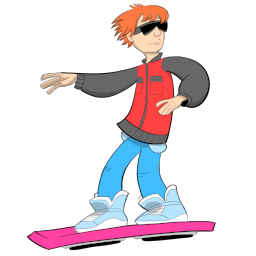
\includegraphics[width=1in]{images/HoverBoard-small.png}
%	\end{wrapfigure}
%
%	We denote the restriction on the hover board's movement by the vector
%	$\mat{3 \\1}$. By this we mean that if
%	the hover board traveled ``forward'' for one hour, it would move along a
%	``diagonal'' path that would result in a displacement of 3 km East and
%	1 km North of its starting location.
%\end{minipage}
%
%\begin{minipage}{\textwidth}
%	\vspace{.5cm}
%	\begin{wrapfigure}{l}{1in}
%	\vspace{-.8cm}
%	
\includegraphics[width=1in]{images/MagicCarpet-small.png}
%	\end{wrapfigure}
%
%	We denote the restriction on the magic carpet's movement by the vector
%	$\mat{1 \\2 }$. By this we mean that if the
%	magic carpet traveled ``forward'' for one hour, it would move along a
%	``diagonal'' path that would result in a displacement of 1 km East and
%	2 km North of its starting location.
%\end{minipage}
%
%\lfoot{\footnotesize Drawings by \url{@DavidsonJohnR} (twitter)}
%
%\vspace{10mm}
%
%% Scenario Section
%\textbf{Scenario One: The Maiden Voyage}
%
%Your Uncle Cramer suggests that your first adventure should be to go visit
%the wise man, Old Man Gauss. Uncle Cramer tells you that Old Man Gauss
%lives in a cabin that is 107 km East and 64 km North of your home.
%
%\vspace{5mm}
%
%\textbf{Task:}
%\par
%Investigate whether or not you can use the hover board and the magic
%carpet to get to Gauss's cabin. If so, how? If it is not possible to
%get to the cabin with these modes of transportation, why is that the case?
%
%%\vspace{5mm}
%% As a group, state and explain your answer(s) on the group whiteboard. Use
%% the vector notation for each mode of transportation as part of your
%% explanation and use a diagram or graphic to help illustrate your
%% point(s).
%\end{iola}
%
%

\end{document}
